% TEX file generated by R with the 'knitr' package
%
% DO NOT EDIT THE TEX FILE DIRECTLY
% ===========================================================================================================
\documentclass[a4paper, notitlepage]{extreport}\usepackage[]{graphicx}\usepackage{xcolor}
% maxwidth is the original width if it is less than linewidth
% otherwise use linewidth (to make sure the graphics do not exceed the margin)
\makeatletter
\def\maxwidth{ %
  \ifdim\Gin@nat@width>\linewidth
    \linewidth
  \else
    \Gin@nat@width
  \fi
}
\makeatother

\definecolor{fgcolor}{rgb}{0.345, 0.345, 0.345}
\newcommand{\hlnum}[1]{\textcolor[rgb]{0.686,0.059,0.569}{#1}}%
\newcommand{\hlstr}[1]{\textcolor[rgb]{0.192,0.494,0.8}{#1}}%
\newcommand{\hlcom}[1]{\textcolor[rgb]{0.678,0.584,0.686}{\textit{#1}}}%
\newcommand{\hlopt}[1]{\textcolor[rgb]{0,0,0}{#1}}%
\newcommand{\hlstd}[1]{\textcolor[rgb]{0.345,0.345,0.345}{#1}}%
\newcommand{\hlkwa}[1]{\textcolor[rgb]{0.161,0.373,0.58}{\textbf{#1}}}%
\newcommand{\hlkwb}[1]{\textcolor[rgb]{0.69,0.353,0.396}{#1}}%
\newcommand{\hlkwc}[1]{\textcolor[rgb]{0.333,0.667,0.333}{#1}}%
\newcommand{\hlkwd}[1]{\textcolor[rgb]{0.737,0.353,0.396}{\textbf{#1}}}%
\let\hlipl\hlkwb

\usepackage{framed}
\makeatletter
\newenvironment{kframe}{%
 \def\at@end@of@kframe{}%
 \ifinner\ifhmode%
  \def\at@end@of@kframe{\end{minipage}}%
  \begin{minipage}{\columnwidth}%
 \fi\fi%
 \def\FrameCommand##1{\hskip\@totalleftmargin \hskip-\fboxsep
 \colorbox{shadecolor}{##1}\hskip-\fboxsep
     % There is no \\@totalrightmargin, so:
     \hskip-\linewidth \hskip-\@totalleftmargin \hskip\columnwidth}%
 \MakeFramed {\advance\hsize-\width
   \@totalleftmargin\z@ \linewidth\hsize
   \@setminipage}}%
 {\par\unskip\endMakeFramed%
 \at@end@of@kframe}
\makeatother

\definecolor{shadecolor}{rgb}{.97, .97, .97}
\definecolor{messagecolor}{rgb}{0, 0, 0}
\definecolor{warningcolor}{rgb}{1, 0, 1}
\definecolor{errorcolor}{rgb}{1, 0, 0}
\newenvironment{knitrout}{}{} % an empty environment to be redefined in TeX

\usepackage{alltt}

% Captions in floating environments
\usepackage{titling}
\usepackage{authblk}
\usepackage{framed}
\usepackage{xcolor}
\usepackage{amsmath}
\usepackage{type1cm}
\usepackage{lettrine}
\usepackage{natbib}
\usepackage{pgfplots}
\usepackage{float}
\pgfplotsset{compat=1.16}

% captions
\usepackage[font=footnotesize,
            labelfont=bf,
            textfont=it,
            margin=.5cm
            ]{caption}

%\setlength{\parskip}{1em}
\edef\restoreparindent{\parindent=\the\parindent\relax}
\usepackage{parskip}
\restoreparindent

% todo notes
\usepackage{todonotes}

% sans font
\usepackage[defaultsans]{droidsans}

% margins
\usepackage[a4paper,margin=2.5cm]{geometry}

\usepackage{setspace}
\onehalfspacing

% pagestyle
\usepackage{fancyhdr}
\usepackage{lastpage}

\fancypagestyle{newchapter}{%
\fancyhf{} % clear all header and footer fields
\renewcommand{\headrulewidth}{0pt}
\renewcommand{\footrulewidth}{0pt}
\rfoot{\ruleline{\fontsize{9}{9}\bfseries Page \thepage\ of \pageref{LastPage}}}
}

\fancypagestyle{firststyle}{
\fancyhf{}
\renewcommand{\headrulewidth}{0pt}
\setlength{\headsep}{10pt}
\renewcommand{\footrulewidth}{0pt}
\lhead{\rulelinel{\fontsize{9}{9}\bfseries \leftmark}}
\rfoot{\ruleline{\fontsize{9}{9}\bfseries Page \thepage\ of \pageref{LastPage}}}
\setlength{\footskip}{20pt}
}

\fancypagestyle{preamble}{
\fancyhf{}
\renewcommand{\headrulewidth}{0pt}
\lfoot{\rulelinel{\fontsize{9}{9}\bfseries \thepage}}
}

\fancypagestyle{ack}{
\fancyhf{}
\renewcommand{\headrulewidth}{0.4pt}
\lfoot{\rulelinel{\fontsize{9}{9}\bfseries \thepage}}
}

\fancypagestyle{empty}{
\fancyhf{}
\renewcommand{\headrulewidth}{.4pt}
\renewcommand{\footrulewidth}{.4pt}
}

% For subcaptions in figures
\usepackage{subcaption}

% For sidewaysfigure
%\usepackage{rotfloat}

% For professional looking tables
\usepackage{booktabs} 

%\usepackage{multirow}
\usepackage{multicol}
%\usepackage{longtable}
%\usepackage{tabularx}

% For \FloatBarrier
\usepackage[section,below]{placeins}

% Linebreaks in tables
\usepackage{makecell}
\usepackage{wrapfig}

% Hyperlinks
\definecolor{darkblue}{rgb}{0.0,0.0,0.4}
\definecolor{darkred}{rgb}{0.5,0.0,0.0}
\usepackage{hyperref}
\hypersetup{
    colorlinks = true,
    linkcolor = darkred,
    anchorcolor = darkred,
    citecolor = darkred,
    urlcolor = darkblue
}
\urlstyle{sf}
% main font
%\usepackage{XCharter} %% cf http://www.khirevich.com/latex/font/
\usepackage[bitstream-charter]{mathdesign}
% For underscores that correspond to the encoding
\usepackage[T1]{fontenc}

% Table of content settings
\setcounter{tocdepth}{2}
\setcounter{secnumdepth}{2}
\usepackage{tocbasic}
\addtotoclist[report.cls]{toc}
\renewcommand*{\tableofcontents}{\listoftoc[{\contentsname}]{toc}}% ToC under control of tocbasic
\AfterTOCHead[toc]{\thispagestyle{preamble}\pagestyle{ack}}
\AfterStartingTOC[toc]{\clearpage}

% Allowed percentages of page a float can use
\renewcommand{\textfraction}{0.05}
\renewcommand{\topfraction}{0.95}
\renewcommand{\bottomfraction}{0.95}
\renewcommand{\floatpagefraction}{0.75}

% Figure names
\renewcommand{\figurename}{Fig.}

% Used for knitr images from Rnw files
\newcommand{\subfloat}[2][default for first parameter: need a sub-caption]{\subcaptionbox{#1}{#2}}

% Typesetting commands
\newcommand{\R}{\textbf{\textsf{R}}}

%%% My additions %%%
\newcommand*\ruleline[1]{\par\noindent\raisebox{.8ex}{\makebox[\linewidth]{\hrulefill\hspace{1ex}\raisebox{-.6ex}{#1}\hspace{1ex}}}}

\newcommand*\rulelinel[1]{\par\noindent\raisebox{.8ex}{\makebox[\linewidth]{\hrulefill\hspace{1ex}\raisebox{-.6ex}{#1}\hspace{1ex}\hrulefill}}}

% change chapters
\usepackage{titlesec}

\titleformat{\chapter}
{\Large\bfseries}
{}
{0.5em}
{\titlerule\, \thechapter. \thispagestyle{newchapter}}

\titleformat{name=\chapter,numberless}
{\Large\bfseries}
{}
{0.5em}
{\titlerule\enspace \thispagestyle{preamble}}
[]

% sections
\titleformat{\section}
{\large\bfseries}
{}
{0.5em}
{\thesection. }
[]

\titleformat{name=\section,numberless}
{\large\bfseries}
{}
{0.5em}
{}
[]

% subsections
\titleformat{\subsection}
{\normalsize\itshape\bfseries}
{}
{0.5em}
{\thesubsection. }
[]

% subsections
\titleformat{\subsubsection}
{\small\itshape}
{}
{0.5em}
{\thesubsubsection. }
[]

\providecommand{\keywords}[1]{\footnotesize\textbf{\textit{Keywords:}} #1}

\newcommand{\copyrightfont}{\linespread{1}\normalfont\rmfamily\fontsize{7}{8}\selectfont}
\newcommand{\ackfont}{\rmfamily\bfseries\fontsize{9}{9}\selectfont}
\renewcommand\Authfont{\normalfont\sffamily\bfseries\fontsize{11}{11}\selectfont}
\newcommand{\datesfont}{\linespread{1}\normalfont\sffamily\fontsize{10}{8}\selectfont}
\newcommand{\titlefont}{\linespread{1}\normalfont\rmfamily\fontsize{22pt}{24pt}\selectfont}

% bib
\setlength{\bibsep}{10pt}
\renewcommand*{\bibfont}{\normalfont\rmfamily\fontsize{9.5}{10}\selectfont} % set font to be sans serif

\pagestyle{firststyle}

\renewcommand*\footnoterule{}

\usepackage{multicol}
\usepackage{etoolbox}
\usepackage{relsize}
\patchcmd{\thebibliography}
  {\list}
  {\begin{multicols}{2}\smaller\list}
  {}
  {}
\appto{\endthebibliography}{\end{multicols}}

\appto\appendix{\addtocontents{toc}{\protect\setcounter{tocdepth}{1}}}

% reinstate the correct level for list of tables and figures
\appto\listoffigures{\addtocontents{lof}{\protect\setcounter{tocdepth}{1}}}
\appto\listoftables{\addtocontents{lot}{\protect\setcounter{tocdepth}{1}}}


\IfFileExists{upquote.sty}{\usepackage{upquote}}{}
\begin{document}




\nocite{ENVS450,devtools,Hmisc,PerformanceAnalytics,ggthemes,RStoolbox,broom,viridis,viridisLite,ggpubr,magrittr,sf,kableExtra,scales,lidR,raster,nvimcom,tidyverse,varhandle,future,rgdal,pbapply,cowplot,bibtex,benchmarkme,parallel,showtext,data.table,wesanderson}

% ===========================================================================================================
% Cover
% ===========================================================================================================

\title{Utilising Supervised Paramatric Classification to Assess the Quality of the UK Rural Road Network using Aerial LiDAR Data}
{\copyrightfont\author{201374125}}
\date{}
    \maketitle
    \thispagestyle{empty}
    \vskip 50pt
\begin{abstract}
\centering\begin{minipage}{\dimexpr\paperwidth-10cm}
    \hrule
    \vskip 5pt
An automated method for the identification of rural road geometric features is presented for use in a national rural road assessment in England. This method uses Government produced LiDAR point cloud data to obtain road surface height, and intensity information. Road centrelines provided by Ordnance Survey are used to enable an automated classification of road surfaces, allowing for road width extraction. Aerial imagery is additionally used to provide luminescence information to aid with road classification. Additional geometric features extracted from the chosen rural roads include the change in road elevation and road surface quality, derived through LiDAR data, and road bend sharpness, derived through the OS Road Centrelines data. The method presented ensures scalability, allowing for an extension beyond the 1km$^2$ area proposed, given access to the appropriate data and suitable computational power. For road classification to be used in width extraction, a unique classification method is proposed, utilising a linear probability model, given points determined to be road surface, derived from the road centreline information. A sampling methodology is implemented, which primarily reduces the computational overhead through a reduction in LiDAR points required for classification. Results were broadly assessed qualitatively and quantitatively giving around a 70\% accuracy in road width measurements. A direct comparison of individual road quality is presented as the Road Quality Index (RQI), which combines the extracted geometric features of roads.
    \vskip 5pt
    \hrule
    \vskip 10pt
\keywords{LiDAR; Aerial Imagery; Linear Probability Classification; Rural Road Quality}
\end{minipage}
\end{abstract}

\vskip 12pt

{\copyrightfont\centerline{\bfseries In Partial Fulfillment of the Requirements for the Degree of}}
{\copyrightfont\centerline{\bfseries Geographic Data Science MSc}}
\centerline{
\includegraphics[width = 100mm]{./template/uolLogo.png}}

% ===========================================================================================================
% Front matter
% ===========================================================================================================

\pagenumbering{Roman}

\newpage
\renewcommand{\abstractname}{Acknowledgements}
\vspace*{\fill}
\begin{abstract}
\centering\begin{minipage}{\dimexpr\paperwidth-10cm}
    \hrule
    \vskip 5pt
    I would like to thank my supervisor Paul Williamson for his continued support throughout the writing of this dissertation. Thank you to John Murray for his help with the various mathematical problems and solutions presented through the methodology, particularly for providing some of the core functions and insights that were essential for this dissertation. I would also like to thank Jean Romain (and package contributors) for his excellent work producing the lidR R package, without which the manipulation of LiDAR data in this paper would have been far more limited. Finally, thank you to Jenny Gibson, who always provides love and support throughout my studies.
    \vskip 5pt
    \hrule
    \vskip 10pt
\end{minipage}
\end{abstract}
\vspace*{\fill}
\thispagestyle{ack}

\tableofcontents

\listoffigures

\listoftables

\chapter*{Definitions}
\begin{multicols}{2}
\begin{itemize}
    \section*{Local Definitions}
\item \textbf{Road:} a section of a full named road that is extracted from Ordinance Survey road centrelines. Often (but not always), a section of road that is in-between two junctions. Due to the nature of roads, it is essential to define a start and end point to ensure no ambiguity. Figure \ref{fig:area_map} gives and overview of what is considered to be a road in this analysis.
\item \textbf{Node:} each road may be split into nodes, defined by the point at which a road changes direction, as indicated on the Ordinance Survey road centrelines, a node may also be the start and end of a road. In computational geometries, nodes are the start and end point of a \texttt{LINESTRING}, which may be part of a \texttt{MULTILINESTRING}.

\section*{Broad Definitions}
    \item \textbf{Light Detection and Ranging (LiDAR):} similar to radar, a laser pulse is sent out of a transmitter on an aircraft or ground vehicle and the light is reflected back to a receiver.
    \item \textbf{Billion Vehicle Miles (BVM):} the total number of miles travelled by all vehicles divided by 1 billion. Typically all traffic is measured in vehicle miles.
    \item \textbf{Digital Terrain Model (DTM):} digital representation of the land surface topography without surface objects.
    \item \textbf{Digital Surface Model (DSM):} digital representation of the land surface capturing all natural and built features.
    \item \textbf{Transport Accessibility:} a measure of the ease of reaching (and interacting with) destinations or activities distributed in space.
    \item \textbf{Social Exclusion:} exclusion from the prevailing social system and its rights and privileges, typically as a result of poverty or the fact of belonging to a minority social group.
    \item \textbf{Read-eval-print loop (REPL):} a simple interactive computer programming environment that takes single user inputs, evaluates them, and returns the results to the user.
    \item \textbf{Root Mean Square Error (RMSE):} the square root of the second sample moment of the differences between predicted values and observed values. Commonly used to measure the difference between sample or population values.
    \item \textbf{Scalability:} the property of a system to handle an increasing amount of work. In this context, a methodology that may handle an increasing area of interest.
\end{itemize}
\end{multicols}

% ===========================================================================================================
% Main matter
% ===========================================================================================================

\cleardoublepage
\pagenumbering{arabic}
\pagestyle{firststyle}

\chapter{Introduction}
\label{ch:introduction}

       \lettrine{R}{oad} usage in the United Kingdom has been steadily increasing by year with the highest ever billion vehicle miles travelled in 2018  \citep[318.1 BVM;][]{departmentfortransport2019}. Characterised by tall hedgerows and winding turns, rural roads in the UK are often unsuitable for higher traffic flow due to the obstruction of view from protected hedgerows, narrow lanes and often poor condition \citep{departmentfortransport2018b}. Due to the abundance of these roads, with "Unclassified" local network roads making up 60\% of all roads in the UK \citep{departmentfortransport2012}, and their varying nature, the national assessment of these roads into appropriate speed limits on an individual basis has been considered impractical \citep{taylor2002}. Due to this, there have been no individual assessments for the majority of rural roads, and instead, given their nature, they are classified as unlit, single carriageway roads and thus assigned a default speed of 60mph \citep{ukgovernment2019a}. Highways England manages the motorways and trunk roads within the UK, but local road networks are maintained by Local Authorities, and as such there is at present no comprehensive information regarding these smaller road networks \citep{highwaysengland2019}. Rural roads in the UK are often cited as by far the most dangerous road type with studies suggesting that up to two thirds of vehicle accidents occur on rural roads \citep{corben2005}.

The Rural Urban Classification defines a rural area as one outside of a settlement with more than a 10,000 resident population \citep{ukgovernment2011}, therefore a road could be considered rural, if either connecting or present within small settlements in the UK. This study will focus particularly on rural connecting roads, outside of rural towns. The purpose of this is to select roads that are unlit, and are unlikely to have been individually assessed, as opposed to roads that are present within more built up rural areas. These roads are considered to likely have the designated national speed limit of 60 mph, and feature hedgerows, narrow road surfaces, and bends, key features to be considered in this dissertation.

A Governmental review of speed policy considered the need for the role of speed and accidents on rural roads to be further addressed \citep{roadsafetyandenvironment2000}, suggesting a framework for individual classification of roads, taking into account local considerations of the road to implement more suitable speed limits. In 2012, draft guidance for rural roads was presented by the Department for Transport suggesting a blanket reduction in rural single carriageway road speed limits from 60mph to 40mph and a reduction to 50mph for lower quality A and B roads \citep{bbc2012}. However, this draft guidance has yet to be implemented, likely due to the costs involved in a blanket change to speed limits. For example, the cost for a complete change in national speed limits from imperial to metric in Ireland cost an estimated €30 million in speed limit signs alone \citep{noctor2004}. These costs suggest that an alternative to blanket implementation may be required.

National speed limits have seen little variation for a number of years, with the majority of roads following the broad criteria for the three main roads types. The three national speed limits are:

\begin{itemize}
\item the 30 mph speed limit on roads with street lighting (sometimes referred to as Restricted Roads)

\item the national speed limit of 60 mph on single carriageway roads

\item the national speed limit of 70 mph on dual carriageways and motorways.
\end{itemize}
\begin{flushright}
    \footnotesize{\citep{ukgovernment2019a}}
\end{flushright}

The \cite{departmentfortransport2013b} outline, in \textit{Setting Local Speed Limits}, that national speed limits are not appropriate for all roads, where local road conditions present the requirement for alternative speed limits. The majority of the rural road network in the UK follows the national speed limit of 60mph for single carriageway roads, and 70mph for dual carriageway roads, despite driver speed often being far below the speed limit. The \cite{departmentfortransport2013b} note that this is especially common on C and Unclassified roads due to the narrow width, frequent bends, junctions and access roads. In 2011, an estimated 66\% of total road deaths in Britain occurred on rural roads, with 51\% on single carriageway rural roads with the national speed limit of 60mph \cite{departmentfortransport2012}.

The \cite{departmentfortransport2013b} suggest that selecting alternative speed limits for single carriageway rural roads should consider:

\begin{itemize}
    \item History of collisions;
    \item The road's function;
    \item Existing mean traffic speed;
    \item Use by vulnerable road users;
    \item The road's geometry and function;
    \item and the road environment, including road-side development.
\end{itemize}

The Road Safety Management Capacity Review \citep{departmentfortransport2018} outlines the current limitations with road safety management, with the lack of defined and measurable safety performance framework, noting that such a framework should set out the long term goal of total prevention of road deaths and injuries, achieving this through a reduction in average speeds on different road types, and an improvement in emergency response times. This review states that at present there is a distinct lack of both urban and rural road hierarchies, which could be used to better match appropriate speed limits, with function, layout and design. Again, this review notes that posted speed limits often allow for speed far in excess of the design limits of single carriageway rural roads, with inappropriate but allowable speed often a contributing factor in rural accidents. Finally the report calls for a review of national speed limits as soon as possible.

A recent development for guidance in setting local speed limits is the production of the \textit{Speed Limit Appraisal Tool} \citep{departmentfortransport2013a}. This tool provides an automated method for the introduction of new speed limits for local councils. This tool takes observed traffic flow, accidents, speeds, descriptive information regarding the network and current costs, outputting projections in these data to advise speed limit changes. While this tool introduces a quantitative method for individual road speed limit assessments, it misses some key features outlined in past government framework proposals \citep[e.g.][]{departmentfortransport2018}, particularly in relation to road geometry.

The innovative methodology presented in this dissertation will focus particularly on the call for an improved understanding of rural road geometry to support the production of appropriate and justified speed limits for rural single carriageway roads, and to inform future requirements for a full rural road hierarchy. Road geometry is defined here as the parameters of roads relating to geometric design, particularly relating to the appropriate road speed, stopping sight distance, road width, road bends and surface quality \citep{jaakkola2008}.

Some road geometric information may be extracted through the readily available OS Road centreline geometries. However, the extraction of road widths poses a complication as this information is not readily available, and automated extraction requires techniques that enable road classification through the data available, either aerial imagery, or LiDAR. Road classification techniques have more recently been aided through the introduction of LiDAR data, as an alternative to aerial imagery classification, allowing for more reliable results due to the presence of additional information that LiDAR provides. The following section outlines LiDAR in this context, and presents how LiDAR may be used to extract these features of roads.

\section{Introduction to LiDAR}
\label{sec:overviewlidar}

Aerial LiDAR data is collected by emitting rapid laser pulses from an aircraft towards the ground which are reflected back, measuring the distance between the aircraft and surface objects at up to 500,000 measurements per second \citep{environmentagency2019}. This method produces a set of highly accurate three dimensional points which collectively are known as a LiDAR point \textit{cloud}. As LiDAR data detects all surface objects, the resultant point cloud produced will include all natural and man made structures, including buildings, roads and trees in addition to the natural variation in the terrain height, known as a digital surface model \citep{hatger2005}.

The main features unique to LiDAR, unlike similar aerial data collection techniques such as true colour imagery are outlined below:

\begin{itemize}
    \item \textbf{Pulses}: LiDAR systems record the data by emitting a laser pulse which is reflected back at the aircraft by ground objects. If the laser hits a solid object such as ground or a building roof, this laser pulse is entirely reflected back towards the aircraft, giving a single point. However, if the laser pulse hits a soft object such as a tree canopy, the pulse may be partially returned, giving multiple return pulses \citep{rottensteiner2003}. Therefore, these multiple pulse returns give information regarding objects at an exact $xy$ location but with varying heights.

    \item \textbf{Intensity}: LiDAR systems also give intensity values for return pulses, which gives information regarding the reflectance of the surface of objects that are hit by the laser pulses. If intensity is given $I$ then reflectance $R$ may be represented as $R = \frac{I}{E_{T}}$ where $E_T$ refers to the first pulse signal intensity \citep{charaniya2004}.

    \item \textbf{Elevation:} In addition to $x$ and $y$ coordinates, the distance between the aircraft and the reflected ground or object is recorded and assigned a $z$ value.
\end{itemize}

\subsection{Benefits over Aerial Imagery}

Rural roads in the UK are often characterised by dense hedgerows either side, with large trees that extend over the road surface. In addition to the reduction in corner visibility on these roads, standard aerial imagery suffers from the road surface being obscured by shadows from these trees and hedgerows, and the tree canopy itself. Additionally, aerial imagery often suffers from obstruction due to clouds \citep{li2016}. Due to the inclusion of pulses with modern LiDAR data, the road surface can often be detected through the canopy by selecting the final pulse returns, the infrared laser pulses also have smaller shadows, due to the narrow scanning angle of LiDAR \citep{wang2009}. Non LiDAR imagery often suffers from scene complexity, where road patterns, vehicles and lane markings reduce road heterogeneity \citep{li2016}.

The 3D $z$ value information provided by LiDAR data allows for the separation of ground and objects on the surface, meaning roads and buildings are often easily separated, despite having similar reflectance \citep{sampath2008}. Additionally, the reflectance of roads is often homogeneous, and distinctly separate from vegetation \citep{clode2004}.

\subsection{Limitations}

LiDAR lacks any texture or spectral information, and often studies in road classification have combined LiDAR with aerial imagery to alleviate this issue \citep{hu2004,zhang2003}, with the inclusion of luminescence information to aid with road classification \citep[e.g.][]{charaniya2004}. LiDAR points are distributed irregularly and with varying density, with point density often higher where flight strips overlap, and tall objects can occlude points, leaving more limited data surrounding trees or buildings \citep{li2016}.

Often road classification methodologies use LiDAR height data to identify kerbs to separate streets from pavement \citep{kumar2013,vosselman2009a}, however rural roads often have no kerb, and are often at the same level as the surrounding vegetation \citep{yadav2018}.

LiDAR data often requires a large amount of processing due to the irregular distribution of points, presence of noise and the number of variables that have to be considered. \cite{yadav2018} note that often papers do not include information regarding the computational time for processing this data which may cause practical limitations at larger scales.



\section{Objective of this Dissertation}
\begin{knitrout}\footnotesize
\definecolor{shadecolor}{rgb}{0.969, 0.969, 0.969}\color{fgcolor}\begin{figure}[b]

{\centering 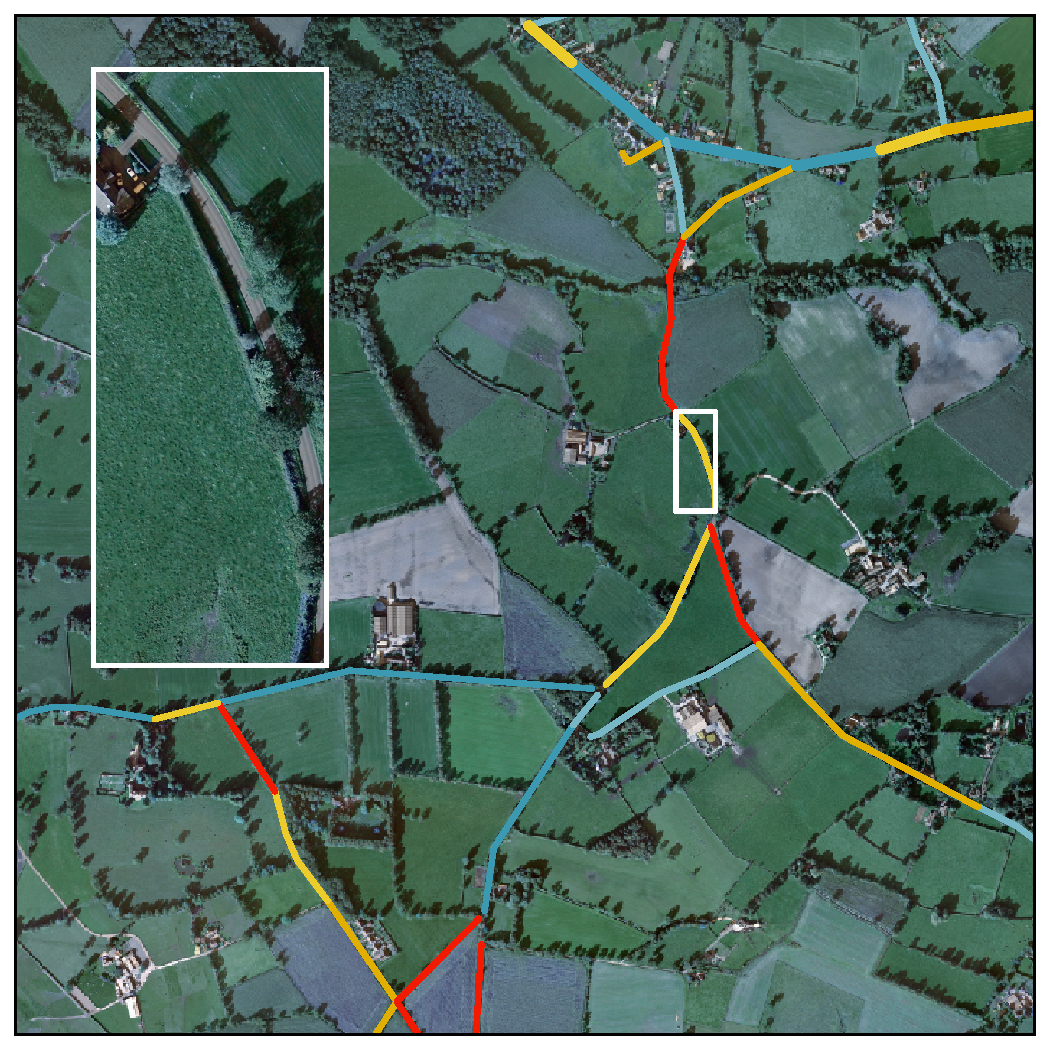
\includegraphics[width=.75\linewidth]{figure/area_map-1} 

}

\caption[Study area highlighting road centrelines]{Study area highlighting road centrelines; each colour represents a separate 'road' as defined by the OS Data provided. Thicker roads are B roads, while thinner are Unclassified. The inset map shows an example road, with features typical of roads within this study area.}\label{fig:area_map}
\end{figure}


\end{knitrout}

This dissertation will present a method for rural road classification and width extraction for a 1km$^2$ region in the North West of England (Figure \ref{fig:area_map}). The methodology is produced in order to ensure scalability and automation, allowing for replication for any area where data is available. Data used will include road centreline geometries, LiDAR point cloud, and aerial imagery to extract road widths through linear probability models. Additionally, this dissertation aims to extract other features of roads such as elevation changes, surface quality, and the sharpness of bends. The extraction of such features aims to build upon past road classification studies, combined with a more refined methodology that aims to ensure a higher accuracy for rural British roads. Unlike previous road classification methodologies, this dissertation aims to focus primarily on road feature extraction, and not the accurate extraction of road locations, as road centerline locations provided by Ordnance Survey already exists. 

\textbf{\textit{Key Aims:}}

\begin{itemize}
    \item Using OS Road and LiDAR Data produce an automated method for determining the characteristics of rural roads that relate to overall road quality. These are;
        \subitem Bend sharpness
        \subitem Road steepness
        \subitem Surface quality
        \subitem Road width
    \item Produce and assess an automated method using LiDAR, aerial imagery and OS road geometry to determine the true width of roads within the chosen study area, outlining the particular limitations and solutions when considering the rural British road network.
    \item Using extracted road features, outline the overall quality of the road network, and allow for direct comparison between each road.
\end{itemize}


This dissertation is organised into chapters, first a literature review, outlining the broad implications of speed limits, rural road networks, and object extraction particularly in relation to LiDAR aerial point clouds. Second, a detailed description of the methodology involved in this dissertation will outline the techniques used to classify road widths, in addition to the other road geometric information. A results section will primarily assess the method for road classification, through sensitivity analysis and some qualitative observations, a section will then explore the findings. Finally a discussion will detail the implications of the findings, and suggest areas for methodological improvement.

\chapter{Literature Review}
\label{ch:literature}

    \lettrine{T}{ypical} road classification techniques have focused purely on urban road networks and involved methods which can be both computationally intensive and time consuming. Given the pressure for a full quantitative assessment of the current speed limits for the rural road network in the United Kingdom, there is a demand to produce comprehensive methods for rural road feature extraction that may be applied nationally. This paper primarily focuses on techniques for assessing the road geometry for roads considered to be rural connecting roads in the United Kingdom. This literature review will first outline the current understanding of the rural road network, considering the role of speed and speed limits in accident likelihood, and a detailed look at current road extraction techniques involving aerial imagery and LiDAR, presenting the key differences and limitations of these studies when considering the rural road network in the UK.

\section{British Rural Road Network}

\cite{taylor2002} conducted a study outlining the key features of British rural roads, in an effort to improve the understanding of the characteristics associated with accident rates, beyond the past \textit{Speed-accident relationship on European Roads} (MASTER) study which primarily consisted of European road data, with limited data for England \citep{baruya1998}. \cite{taylor2002} identify key features of 174 selected rural British roads across England which they use to classify roads into certain categories. This data was obtained through drive-through video recordings.

Features that \cite{taylor2002} suggest to consider in an analysis of British rural roads are given on Table \ref{tab:roadfeatures}. This study manually measured the road width for each site, and to determine the "hilliness" of roads, the number of 10m contour lines crossed were counted to give the total change in height.

\begin{table}[htbp]
    \centering
\fontsize{9}{10}\selectfont
\caption{Features identified as important to British rural road analysis.}
\label{tab:roadfeatures}
\begin{tabular}{ll}
\toprule
\textbf{Type of data} & \textbf{Examples} \\
\midrule
Discrete data & \begin{tabular}[c]{@{}l@{}}Type of junction \\ Minor junctions \\ Accesses \\ Number of bends, classified into:\\ \quad Sharp (warning signposts) \\ \quad Medium \\ \quad Slight\end{tabular} \\ \\
Semi-continuous data & \begin{tabular}[c]{@{}l@{}}Lighting \\ Reflecting road studs \\ Kerbs \\ Number of lanes \\ Road markings \\ Land use\end{tabular} \\ \\
Continuous data & \begin{tabular}[c]{@{}l@{}}Visibility \\ Verge width and type \\ Roadside type \end{tabular}                                                                                                                              \\ \bottomrule
    \footnotesize{\citep{taylor2002}}
\end{tabular}
\end{table}

\cite{taylor2002} categorised these roads into four key groups:

\begin{itemize}
    \item \textbf{Group 1:} Roads which are very hilly, with a high bend density and low traffic speed. \textit{These are low quality roads.}

    \item \textbf{Group 2:} Roads with a high access density, above average bend density and below average traffic speed. \textit{These are lower than average quality roads.}

    \item \textbf{Group 3:} Roads with a high junction density, but below average bend density and hilliness, and above average traffic speed. \textit{These are higher than average quality roads.}

    \item \textbf{Group 4:} Roads with a low density of bends, junctions and accesses and a high traffic speed. \textit{These are high quality roads.}
\end{itemize}

This study therefore attempted to outline a rural road hierarchy in relation to road function, and certain road geometries, which addresses issues outlined in the Government's review of speed policy \citep{roadsafetyandenvironment2000}. However, due to the nature of the data collection for this study, time constraints mean that producing a full road hierarchy for all rural roads within England using this methodology is impractical.

\subsection{Rural Speed Limits}
An observation of 270 single carriageway rural roads in England found that the distribution of mean speeds was wide, and often significantly below the 60mph limit \citep{departmentfortransport2006}. Accidents on rural roads often occur within the 60 mph speed limit meaning a distinction between what is an appropriate speed should be made that does not relate to a given speed limit. \cite{baruya1998} suggest a distinction between both \textit{excess} and \textit{inappropriate} speed. \textit{Excess} when driving above the speed limit, and therefore directly breaking the law; \textit{inappropriate} speed, when driving too fast for the conditions of the road, not necessarily above the speed limit, often considered dangerous driving. A study by the \cite{departmentfortransport2013b} assessed the impact of inappropriate speed on rural roads, which contributed to 20\% of all crashes on minor rural roads with a 60mph limit, whereas excess speed accounted for around 16\% of collisions. The \cite{departmentfortransport2013b} note that this high proportion of inappropriate speed on rural roads reflects the inappropriate speed limits that are given on the majority of rural roads

The Department for Transport found that rural roads account for around 66\% of all road deaths, despite accounting for around 42\% of the total distance travelled by all vehicles. Notably 51\% of all deaths in Britain in 2011 occurred on rural single carriageway roads, with the national speed limit of 60mph \citep{departmentfortransport2011}. 

\subsection{Speed, Road Geometry and Accidents}

Lowering the speed limit on roads has been shown to result in an overall reduction in the average speed of vehicles. \cite{finch1994} found that a reduction in the speed limit of a road resulted in a mean speed reduction of around one quarter of the difference, noting that drivers will often obey speed limits that they determine to be reasonable. A reduction in average speed subsequently leads to a reduction in road traffic accidents \citep{finch1994,taylor2002}. \cite{taylor2000} produced a model to predict accident frequencies given the proportion of drivers exceeding the speed limit and the average speed, finding that excess speed and a higher speed limit were both associated with a higher accident frequency.  Particularly, the risk of death at various speeds has been assessed in various studies, \cite{richards2009} found that at 60mph the risk of a driver dying in a head on collision between two cars is around 90\%, but with a reduction in speed, this drops to around 50\% at 48mph.

\cite{taylor2000}  demonstrated that traffic flow, link length, and the number of minor junctions all directly increased the number of accidents, while wider roads were associated with a reduction in the number of accidents. The \textit{MASTER: Speed-accident relationship on European roads} \citep{baruya1998}, assessed road geometry and other features of rural roads in Europe, however road data for the United Kingdom was limited to a small area in the South East, suggesting that a comprehensive methodology for the extraction of UK rural road geometry is required for a more comprehensive study.

Newer developments like the Speed Limit Appraisal Tool mean that automated and quantitatively informed speed limits may be imposed on rural roads. However, this tool does not take into account key features such as road geometry, and simply builds on existing speed data and accidents \citep{departmentfortransport2013a}. 

\section{LiDAR Data Classification}

Aerial LiDAR classification typically follows two objectives, the classification of ground and non-ground points, and the classification of surface objects, including buildings, trees or roads \citep{charaniya2004}. Classification takes two forms, \textit{supervised} and \textit{unsupervised}, supervised classification taking a \textit{training} dataset, and using it to estimate the parameters associated with the outcome hoping to be classified. These parameters are then used on unknown data, with a similar distribution to the training set, and used to classify features \citep{charaniya2004}.

\subsection{Digital Terrain Models}
\label{subs:dtm}

Early LiDAR classification primarily focused on the production of digital terrain models (DTM) \citep[e.g.][]{kraus1998,maas1999,elberink2000}, by segmenting vegetation, and man made structures from ground. This dissertation will utilise a recent method for DTM production in order to classify ground and non ground points for subsequent road classification. The method chosen was proposed by \cite{zhang2016} using \textit{cloth simulation} to generate a DTM from LiDAR data. This algorithm, unlike other filtering algorithms, allows for a simplistic input, without the need for numerous parameters to ensure an accurate DTM. This method consists of four main steps:

\begin{itemize}
    \item \textit{Initial State.} A simulated \textit{cloth}\footnote{Used in 3D modelling, a simulation of particles with a mass, connected by a mesh, following Newton's Second Law: $\vec{F}=m \vec{a}$ \citep{karthikeyan2001}} is placed above the inverted LiDAR measurements. A series of points that lie flat to the surface and are allowed to move based on the influence of gravity.
    \item The displacement of each LiDAR point is calculated under the influence of gravity, meaning some points appear below ground measurements.
    \item \textit{Intersection check.} For any points detected as being under the ground, they are moved to ground level and set to be unmovable.
    \item \textit{Considering internal forces.} Movable points are moved according to neighbouring points.
\end{itemize}

Quantitative accuracy assessment of this methodology by \cite{zhang2016} gave results similar to top existing DTM production algorithms, but with a far more simplistic implementation, and reduced computation times.

\subsection{Feature Classification}

Developments in LiDAR enabled the possibility of classification beyond ground and non-ground, by using laser intensity information and multiple returns, features of more advanced LiDAR systems. The TopEye system used by \cite{axelsson1999} allowed for classification of buildings and electrical power-lines using reflectance to obtain radiometric information about the area and note that this can be used to separate paved area from grassland. Power lines in particular benefited from the multiple returns produced by the LiDAR system used as they often gave one return from the power line, and one from ground.

Vegetation in particular exhibits multiple returns, whereas most man made surface objects do not. By considering the number of returns and homogeneous height variation \cite{hui2008} were able to categorise surface vegetation into both high vegetation, low vegetation as well as smooth man made surfaces.

\section{Road Classification}

In comparison to the extraction of vegetation and buildings from LiDAR, the extraction of roads poses far more of a challenge, due to there being less prominent height differences \citep{vosselman2009a}. Road classification is essentially a data clustering method to categorise data into road and non-road points, enabled through discovering patterns and relationships between variables and validation of findings \citep{saeedi2009}. Clustering may be achieved through various algorithms, categorised generally into partitioning methods, hierarchical methods, density-based methods, grid-based methods, and model-based methods \citep{saeedi2009}. \cite{yadav2018} note that the periodic assessment of roads is important due to the changing traffic load, which is generally increasing over time, and new automated techniques will enable this in areas where in the past it had not been feasible. Due to the heterogeneous nature of certain roads types, the road environment is often complex, meaning collection and accurate processing of road features is challenging \citep{yadav2018}. 

\subsection{Aerial Imagery}

Road classification methodologies have historically used purely aerial imagery, providing only road pixels and 2D location information \citep{yadav2018,ferchichi2005,wan2007}. Such techniques rely solely on image texture analysis of the coloured pixels \citep{dubes1992}, and appear to be focused entirely in urban settings. Additionally, the methods proposed in aerial image classification fail to address the differentiation between road and pavement, simply classifying building and non-building, rather than roads.

\subsection{LiDAR Road Classification}

Intensity, elevation and the inclusion of multiple returns in LiDAR data enabled methods for categorising roads, and differentiating them from the surrounding ground, despite the similar elevation \citep{clode2004}.

The majority of current road classification techniques using LiDAR have focused on unsupervised classification, often with the goal in vehicle automation using mobile LiDAR data \citep[e.g.][]{yadav2018,kumar2013,smadja2010,jaakkola2008}, and applications using aerial LiDAR have also followed this trend for unsupervised classification \citep{clode2004,vosselman2009}.

Many methods for road classification from LiDAR follow similar patterns, first identification of ground points through height data, then DTM extraction through interpolation, followed by classification based on the attributes of the point cloud \citep{vosselman2009}. \cite{jaakkola2008} produced a methodology using mobile LiDAR data to classify road edges by segmenting kerbstones based on the height gradient along the scanned profile. However, this mobile LiDAR classification required driving speeds of 20km/h to 50km/h, and lengthy computation times. Additionally noted by \cite{yoon2009} in a similar study. Ground based LiDAR collection techniques often provide a resolution far higher than aerial LiDAR data, however the time taken for a comprehensive coverage of all British rural roads would not allow for its use in a national road assessment.

Other unsupervised road classification techniques rely on the detection of planar or smooth surfaces at ground level, indicative of man made objects which, unlike vegetation, do not display sharp variation in height values \citep{vosselman2004,darmawati2008}.

\subsection{Supervised Methods}\label{subsec:supervised}

\cite{guan2013} used both aerial imagery and LiDAR data in combination with a training dataset to classify urban roads. The training dataset gave human labelled features, and used to train a maximum likelihood classification model. \cite{matkan2014} extracted roads from LiDAR using a Support-vector Machine (SVM) classification. Training samples enabled classification into roads, trees, buildings, grassland and cement. Accuracy was determined through testing on three known road datasets, the number of LiDAR points correctly categorised ranged from 63\% to 66\% depending on the classification. \cite{ferraz2016} used supervised random forest classification to detect large-scale forest roads using LiDAR. They note particularly that given the scale of these roads, the efficiency of road extraction is most important, managing to achieve 80\% accuracy with individual roads processed at 2 minutes per kilometer. Despite being forest roads however, the canopy was often not obscuring roads due to their reasonably wide surface, and as such this method produced inaccuracies in areas where the canopy was dense and covering the detected road. \cite{charaniya2004} trained a mixture of Gaussian models using key features of both LiDAR and aerial imagery data. They found that for classification of buildings and roads, the key features of LiDAR that enable extraction were the height, intensity, and the number of returns, in addition to luminescence information obtained from the aerial imagery. Results correctly categorised from 66\% to 84\% of LiDAR points when compared with a labelled dataset.

These supervised techniques give insight into the feasibility for rural road extraction, given a dataset of known road centrelines. With improvements to the quality of LiDAR data more recently, a methodology for road feature extraction using road centrelines and LiDAR may more comprehensively include features that distinguish roads from surrounding objects, including intensity, the number of returns, and aerial luminescence.

\subsection{Rural Road Extraction}

Many recent road extraction techniques have relied on the segmentation between roads and buildings, relying on a clear height difference between road and non-road surfaces \citep{kumar2013}, a feature uncommon to rural roads. Rural road classification therefore must rely on alternative features of roads, notably the difference in intensity produced by vegetation compared with the surface of man made objects, explored in various studies \cite[e.g.][]{vosselman2000}. Additionally, overhanging tree canopies are uncommon features of roads that have been previously classified, and as such, a methodology for classifying rural British roads must take this limitation into particular consideration.

\section{Overview of this Dissertation}\label{sec:overview}

This dissertation aims to extract key features of a selection of rural roads in England through a combination of LiDAR point clouds, OS open road geometries, and aerial imagery, selecting road features considered to be important in past literature and government reviews. The key features considered when determining road quality are;

\begin{itemize}
    \item \textbf{Width:} Narrower roads are associated with an increased number of accidents in many studies of rural roads \citep{taylor2002,aarts2006,taylor2000}
    \item \textbf{Surface quality:} Poor quality road surfaces have been shown to increase the number of road traffic accidents \citep{fleming2009}
    \item \textbf{Blind corners/winding roads:} Blind corners increase the risk of accidents, and higher speeds mean stopping distances are often above the distance visible around rural road corners in the UK. Blind corners are particularly an issue due to the tall hedgerows that often bank rural roads  \citep{aarts2006,wu2013}
    \item \textbf{Road Steepness:} Steeper roads have an increased skid risk, and their quality is more likely to deteriorate \citep{moore2006,viner2004}
\end{itemize}

While the focus of past road classification methods typically aim to classify the entire road surface, this isn't necessary for the feature extraction of roads as proposed in this dissertation. To extract roads widths, only LiDAR points at each edge of the road surface are required, and points along the road surface may be sampled at regular intervals, removing the majority of unnecessary LiDAR points and improving computation time, often a key limitation when working with LiDAR data \citep{zhang2018}. Additionally, this paper aims to concentrate on a supervised classification of roads, by taking known centreline locations, many LiDAR points may be excluded, and remaining points concentrated towards the centre of the centrelines may be used as a training data set. Unlike road widths, other road features do not require classification with the inclusion of known road geometries. Road bends may be determined through the existing road linestrings, while surface quality and road steepness may be extracted at known road locations in the LiDAR point cloud. The method as presented aims to allow for the potential expansion beyond the dataset considered in this analysis, providing the requisite data is available.

\chapter{Methodology}
\label{ch:methods}

    \lettrine{T}{his} dissertation primarily makes use of the free open source statistical language \R{} \citep{parallel}. Managing the large LiDAR datasets from my personal computer was made possible through the \texttt{lidR} \R{} package \citep{lidR}. Further details regarding the \R{} environment and computer setup used for this dissertation are given in \textbf{Appendix \ref{a:code}}. Also given in \textbf{Appendix \ref{a:code}} are the code snippets utilised in this methodology, for many equations, the relevant code is given as a reference to the appendix location, in the form \textbf{A.x.x}. Due to the nature of the functions used in this analysis, a single function often contains multiple equations, and so a reference to a particular appendix number may be repeated.

\section{Data}
\label{sec:data}



LiDAR point cloud data was downloaded through the \href{https://data.gov.uk/}{UK Government's open data repository} which uses the \href{http://www.nationalarchives.gov.uk/doc/open-government-licence/version/3/}{Open Government Licence}, allowing for:
    \begin{itemize}
        \item Copying, publishing, distributing and transmission of the data
        \item Adaptation of the data
        \item Commercial and Non-commercial use of the information
    \end{itemize}

    LiDAR data used in this paper is available \href{https://data.gov.uk/dataset/977a4ca4-1759-4f26-baa7-b566bd7ca7bf/lidar-point-cloud}{\textsc{here}} under this licence \citep{ukgovernment2019}. This data was given as a compressed LAS file format (\texttt{.laz}), the \R{} package \texttt{lidR} provided the function \texttt{lidr::catalog()} which enabled each separate \texttt{.laz} to be combined into one object of class \texttt{LAScatalog}. Analysis on this object could then be split into chunks (selected as 500m$^2$), allowing for multi-core threading to speed up analysis, and a reduction in the memory overhead when reading in data, often a limitation of the \R{} language as objects are stored entirely into memory when read \citep{wickham2014}. The \texttt{LAScatalog} object did not require the compressed \texttt{.laz} files to be read into memory as \texttt{.las} files, meaning memory limitations were far less of a problem.

    Aerial imagery was downloaded through \href{https://digimap.edina.ac.uk/}{Digimap\textsuperscript{\textregistered}
    } which uses the \textit{Aerial Digimap Educational User Licence}, allowing for free use of the data for educational purposes \citep{theuniversityofedinburgh2019}.

Road centreline geometries were accessed through the \href{https://www.ordnancesurvey.co.uk/business-and-government/products/opendata.html}{Ordnance Survey Open Data repository} which shares the Open Government licence. These were downloaded in the GeoPackage format (\texttt{.gpkg}) nationally and cropped to the extent of the LiDAR point cloud data.

\section{LiDAR Preprocessing}

The total number of LiDAR points used in this study is 9,419,272. All LiDAR data has a vertical accuracy of +/-15cm Root mean square error (RMSE). An overview of the LiDAR data selected for this study is given on Table \ref{tab:lidartab}. The variables of primary interest are:

\begin{itemize}
    \item \textbf{z:} The distance a laser pulse is reflected back to to scanner, calculated by the time taken for a return pulse to be detected.
    \item \textbf{Intensity:} The amplitude of the return pulse, reflected back by the surface terrain or objects.
	\item \textbf{ReturnNumber:} A number of range 1-5, indicating for a point, the corresponding order of a reflected laser pulse. A return number of 1 indicates the first return for a pulse (and highest $z$ value), a return number of 5 indicates the last return (and lowest $z$ value).
	\item \textbf{NumberOfReturns:} The number of return pulses for a single laser pulse (maximum of 5).
    \item \textbf{Classification:} A number given to a point indicating a specific numeric classification. Of interest in this study is a classification of 2, indicating a ground point. More information is given by \href{http://desktop.arcgis.com/en/arcmap/10.3/manage-data/las-dataset/lidar-point-classification.htm}{\cite{esri2019}}, which outlines numerical classifications for various vegetation types and man made structures.
\end{itemize}



\begin{table}[!h]

\caption{\label{tab:lidartab}LiDAR Point Cloud Summary Data}
\centering
\fontsize{9}{11}\selectfont
\begin{tabular}{lrrrr}
\toprule
\textbf{ } & \textbf{Mean} & \textbf{SD} & \textbf{Min} & \textbf{Max}\\
\midrule
Z & 80.58 & 5.97 & 64.85 & 115.79\\
Intensity & 177.10 & 124.85 & 1.00 & 4064.00\\
ReturnNumber & 1.47 & 0.95 & 1.00 & 5.00\\
NumberOfReturns & 1.94 & 1.42 & 1.00 & 5.00\\
ScanDirectionFlag & 0.50 & 0.50 & 0.00 & 1.00\\
EdgeOfFlightline & 0.00 & 0.03 & 0.00 & 1.00\\
Classification & 3.04 & 1.70 & 1.00 & 8.00\\
ScanAngleRank & -2.01 & 13.16 & -22.00 & 22.00\\
\bottomrule
\end{tabular}
\end{table}



\subsection{Last Pulse}

The LiDAR point cloud data used in this paper gives the values for 5 pulse returns. The canopy above roads may be excluded through ignoring early pulses (higher Z values), therefore only the last pulse values for any point are selected, taking only points where the \textbf{ReturnNumber} equals the \textbf{NumberOfReturns}. Last pulse points may be expressed as;

$$
\mathbf{p}_{i}=(l p x, l p y, l p z, l p i),
$$
\begin{flushright}
    \footnotesize{\ref{code:lidr_clean}}
\end{flushright}

\noindent where $\mathbf{p_i}$ is a single instance of a LiDAR point within the chosen point cloud, $lpx$ is the last pulse $x$ coordinate, $lpy$ the last pulse $y$ coordinate, $lpz$ the last pulse $z$ coordinate, and $lpi$ the last pulse intensity value.

\subsection{Normalisation}

Ground points were classified using the Cloth Simulation Filtering (CSF) algorithm, as described in \cite{zhang2016}. Points were already classified in the data provided, however, as the classification technique was unknown, reclassification was considered necessary. The general implementation simulates the movements of a piece of cloth lying over the inverse of a point cloud, as the point cloud is flipped, the cloth settles beneath ground points, while covering points that lie separate to the ground, essentially forming a digital terrain model (DTM), cloth simulations are described in more detail in \cite{bridson2005} and subsection \ref{subs:dtm}. The CSF algorithm is given;

$$
X(t+\Delta t)=2 X(t)-X(t-\Delta t)+\frac{G}{m} \Delta t^{2},
$$
\begin{flushright}
    \footnotesize{\ref{code:lidr_clean}}
\end{flushright}



\noindent where $m$  is the mass of a single LiDAR point (set to 1), $\Delta t$ is the time step between points and $G$ represents the gravity constant. The implementation of this algorithm was given as part of the \texttt{lidR} package. Reclassification resulted in an increase in the number of classified ground points by 50.77\%. Reflecting primarily the simplification of existing classifications into ground and non-ground.


With the classification of ground points, (given $\mathbf{Classification} = 2$), a full DTM may be produced through spatial interpolation of the classified points.  Interpolation uses the inverse distance weighting and $k$ nearest neighbours algorithms to produce the DTM. Nearest neighbours were selected as $k = 10$, with $q = 2$ for the inverse weighting, and used to produce a DTM with a resolution of 1m$^2$. This particular technique was selected over more comprehensive methods such as kriging as the number of points is very high, and the small benefit of kriging was considered minimal compared with the increase in computational load. The $z$ values from the DTM were then subtracted from the LiDAR point cloud, leaving a normalised point cloud. This ensures that when extracting height information, any observed values are due to objects on the surface of the terrain, and not due to the lie of the terrain itself.

\subsection{Points Extent}

With the normalised last pulse point cloud, the point cloud was clipped to within a 30m extent of each known road location, using the OS road shapefiles;
\[
\begin{aligned}
   \textbf{p}_i \in \left[A(r_i) \times 30m^2\right],
\end{aligned}
\]
\begin{flushright}
    \footnotesize{\ref{code:extract_buff}}
\end{flushright}

\noindent where $A(r_i)$ are the geometric areas of each road in the study area. Selecting a 30m extent ensured that even with slight inaccuracy in road location, the road LiDAR points would likely not be excluded. A large number of unimportant points were therefore removed, saving on computational resources. Additionally this extent ensured that both road and non road points were included, but reduced the chance of false positives from occurring as fewer non road points were now included in the analysis.


\subsection{Noise Filtering}\label{subsec:noise}

Intensity noise was filtered through area based outlier detection, measuring the 95th percentile values within a 10m$^2$ area, and removing all points above the 95\% percentile. This can be expressed as;

\[
    \begin{aligned}
\mathbf{c}_{k} = \Big(\mathbf{p}_i \in \Big[\frac{95}{100} \times lpi\Big]\Big) \\
A\left(\mathbf{c}_{\mathbf{k}}\right)=10 m^{2}
\end{aligned}
\]
\begin{flushright}
    \footnotesize{\ref{code:las_filter_noise}}
\end{flushright}

\noindent
where $\mathbf{c}_k$ represents a 10m$^2$ selection of LiDAR points, where each point $(\mathbf{p}_i)$ has an intensity value within the 95\% percentile intensity for all original points in $\mathbf{c}_k$.

\subsection{LiDAR Catalog}

As mentioned in Section \ref{sec:data}, objects of class \texttt{LASCatalog} enabled more efficient processing by allowing the LiDAR point cloud to be processed in predefined batch sizes. Considering a collection of processed LiDAR points; last pulse, normalised, clipped to 30m road extents, and intensity noise filtered. Points were then grouped into 500m$^2$ areas;

\[
\begin{aligned}
\mathbf{C}_{N}=\left\{\mathbf{c}_{1}, \mathbf{c}_{2}, \ldots, \mathbf{c}_{k}\right\} \\
A\left(\mathbf{C}_{N}\right)=500 m^{2}, \\
\end{aligned}
\]
\begin{flushright}
    \footnotesize{\ref{code:las_filter_noise}}
\end{flushright}

\noindent and each 500$m^2$ area collectively represents the overall processed point cloud;

\[
\begin{aligned}
\mathbf{S}=\left\{\mathbf{C}_{1}, \mathbf{C}_{2} \ldots, \mathbf{C}_{N}\right\}.
\end{aligned}
\]
\begin{flushright}
    \footnotesize{\ref{code:comb_ctg}}
\end{flushright}

\section{Road Analysis}
\label{sec:road-extraction}

The preprocessed LiDAR data was combined with the OS road shapefiles and aerial imagery to obtain a set of criteria to assess the chosen road network. A summary of the information provided alongside OS road shapefiles is given on Table \ref{tab:roadstab}. While both \texttt{roadNumberTOID} and \texttt{roadNameTOID} do provide true road identification for many roads, this was not true for each road in the area chosen. Due to this, it was impossible to identify what could be considered an individual road, meaning a \textit{road} will now be defined as indicated on Figure \ref{fig:area_map}, selected based on the shapefile geometry provided.



\begin{table}[!h]

\caption{\label{tab:roadstab}OS Roads Data Summary}
\centering
\fontsize{9}{11}\selectfont
\begin{tabular}{ll}
\toprule
\textbf{Variable} & \textbf{Example}\\
\midrule
id & idE381337E-E88D-4232-8CAD-F543F178EBE4\\
endNode & id42B6F387-D838-445C-AA7A-6558362B7B9F\\
startNode & idC8EE8B4C-D965-436A-BA02-A0925A6EA1B8\\
roadNumberTOID & osgb4000000013398492\\
roadNameTOID & \\
fictitious & FALSE\\
roadClassification & B Road\\
roadFunction & B Road\\
formOfWay & Single Carriageway\\
length & 241\\
loop & FALSE\\
primaryRoute & FALSE\\
trunkRoad & FALSE\\
roadClassificationNumber & B5392\\
name1 & \\
name2 & \\
roadStructure & \\
\bottomrule
\end{tabular}
\end{table}



The roads in this paper consist of these functions; 

\begin{itemize}
\item B Road
\item Minor Road
\item Restricted Local Access Road
\item Secondary Access Road
\item Local Road

\end{itemize}

B roads are classified roads, while other functions are unclassified. All roads are single carriageway, and so for the purpose of this analysis it is assumed they likely have the default national speed limit of 60mph. All \textit{Restricted Local Access Roads} were removed, as were roads with a length of less than 50m, often those clipped by the extent of the LiDAR data.

\section{Road Angles}\label{sec:angles}

The angle of each bend in a road was identified through the nodes produced in the creation of the road shapefiles. First the road linestrings were split into points, with coordinates representing each node within a road, a point at which the orientation of the linestring is altered, (See Figure \ref{fig:bearingang1} and \ref{fig:bearingang2} for illustrations of road nodes).

The direction of a road was considered to be the \textit{bearing angle} $\hat \theta$, from a node $\mathbf{N}_i = \left(x_{i}, y_{i}\right)$ to a node $\mathbf{N}_{i+1} = \left(x_{i+1}, y_{i+1}\right)$, with the angle measured in a clockwise direction from north. This is represented on Figure \ref{fig:bearingang1}.

    \begin{figure}[htbp]
        \centering
\begin{tikzpicture}[scale=7]
    \filldraw (.2,.4) circle[radius=.3pt] node [below left] {$\mathbf{N}_{i}$};

\draw[-] (0.1,.4) -- (0.3, .4);
\draw[-] (0.2,.3) -- (0.2, .5) node[above] {$N$};

\filldraw (.8,.7) circle[radius=.3pt] node [above right] {$\mathbf{N}_{i+1}$};

\draw[-] (0.2,.4) -- (0.8, .7);

    \draw[<-] (0.28,.44) arc (45:90:.111);
    \node[] at (.25,.5)  {$\hat \theta_i$};
\end{tikzpicture}
\caption[Bearing Angle ($\hat \theta_i$) between two sequential road nodes.]{Bearing Angle ($\theta$) between two sequential road Nodes; $\mathbf{N}_{i}$ and $\mathbf{N}_{i+1}$. North is given by $N$.}\label{fig:bearingang1}
\end{figure}


To find the angle $\hat \theta$, the node $\mathbf{N}_{i+1}$ can be represented into relation to node $\mathbf{N}_{i}$ as;

$$
\left(x_{i+1}, y_{i+1}\right)=\left(x_{i}+r \sin \theta, y_{i}+r \cos \theta\right)
$$

\noindent where $r$ is the length of the line segment $N_{i}N_{i+1}$. Rearranging the equation for $\theta$ gives;

$$
    \tan \theta=\frac{x_{i+1}-x_{i}}{y_{i+1}-y_{i}}
$$

\noindent this equation can be rewritten to calculate the value of $\theta$ using the $\mathit{atan2}$ function;

$$
\theta=\mathrm{atan} 2\left(x_{i+1}-x_{i}, y_{i+1}-y_{i}\right) \in[-\pi, \pi]
$$


\noindent finally the bearing angle $\hat \theta \in[0,2 \pi]$ may be obtained by the addition of 2$\pi$ to any value below 0;

\[
    \begin{aligned}
\hat \theta=\left\{\begin{array}{ll}{\theta,} & {\theta \geq 0} \\
{2 \pi+\theta,} & {\theta<0}\end{array}\right.
\end{aligned}
\]
\begin{flushright}
    \footnotesize{\ref{code:road_angles}}
\end{flushright}

With the bearing angle of the first line segment ($\hat \theta_{1}$) for a particular road, the change in orientation of the second  line segment between nodes $\mathbf{N}_2$ and $\mathbf{N}_3$ may be given;

\[
\begin{aligned}
\hat{\theta}_2= &\mathrm{atan} 2\left(x_{3}-x_{2}, y_{3}-y_{2}\right) - \\
&\mathrm{atan} 2\left(x_{2}-x_{1}, y_{2}-y_{1}\right),
\end{aligned}
\]
\begin{flushright}
    \footnotesize{\ref{code:road_angles}}
\end{flushright}

\noindent or simply written as $\hat \theta_{2} = \hat \theta_{2} - \hat \theta_{1}$, with additional nodes following the pattern $\hat \theta_{i} = \hat \theta_{i} - \hat \theta_{i-1}$. Figure \ref{fig:bearingang2} illustrates this for nodes 1 to 3, indicating the bearing angle $\hat \theta_2$ in relation to the bearing angle $\hat \theta_1$, rather than in relation to the north ($N$).

    \begin{figure}[htbp]
        \centering
\begin{tikzpicture}[scale=7]

    \filldraw (.2,.4) circle[radius=.3pt] node [below left] {$\mathbf{N}_1$};

\draw[-] (0.1,.4) -- (0.3, .4);
\draw[-] (0.2,.3) -- (0.2, .5) node[above] {$N$};

\filldraw (.8,.7) circle[radius=.3pt] node [above left] {$\mathbf{N}_{2}$};
\filldraw (.9,1) circle[radius=.3pt] node [above right] {$\mathbf{N}_{3}$};

\draw[-] (0.2,.4) -- (0.8, .7);
\draw[-] (0.8,.7) -- (.9, 1);

    \draw[<-] (0.28,.44) arc (45:90:.111);
    \node[] at (.25,.5)  {$\hat \theta_{1}$};

\draw[dotted] (0.8,.7) -- (1, .8);

    \draw[<-] (0.9,.75) arc (45:90:.1);
    \node[] at (.88,.8)  {$\hat \theta_{2}$};
\end{tikzpicture}
\caption[Bearing Angle between the first ($\mathbf{N}_1$), second ($\mathbf{N}_2$) and third node ($\mathbf{N}_3$) of a road.]{Bearing Angle between the first ($\mathbf{N}_1$), second ($\mathbf{N}_2$) and third node ($\mathbf{N}_3$) of a road; giving $\hat \theta_1$ in relation to the north ($N$), and $\hat \theta_2$ in relation to the bearing angle $\hat \theta_1$.}
\label{fig:bearingang2}
\end{figure}

 As the bearing angle between the first two nodes gives only the initial direction of the road, this was set to zero; $\hat \theta_{1} = 0$. In the final analysis, for each road the maximum bearing angle between any two nodes was selected, as well as the average bearing angle between all nodes.

\section{Road Node Elevation Change}\label{sec:elev}

The elevation change between two road node points was calculated by first selecting non-normalised LiDAR points at a geometric node within a 1m$^2$ area. LiDAR points were then filtered by those only classified as ground, and with only a single return, to reduce the likelihood of inaccurate $z$ values from canopy or other vegetation and vehicles. The mean $z$ value of points were found for each node, and elevation change between each node was calculated;
\[
\begin{aligned}
    \Delta e(\mathbf{N}_i, \mathbf{N}_{i+1}) = \Delta \left\{\begin{array}{ll}
    \overline{spz} \in  \left[A(\mathbf{N}_i)\times 1m^2\right], \\
    \overline{spz} \in  \left[A(\mathbf{N}_{i+1})\times 1m^2\right]
\end{array}\right.,
\end{aligned}
\]
\begin{flushright}
    \footnotesize{\ref{code:height_change}}
\end{flushright}

\noindent where $spz$ are the $z$ values for ground classified points with a single return, and $\Delta e(\mathbf{N}_i, \mathbf{N}_{i+1})$ is the change in elevation between sequential nodes $\mathbf{N}_i$ and $\mathbf{N}_{i+1}$, taking the change in mean single return pulse point $z$ values ($\overline{spz}$) within a 1m$^2$ buffer of each node. For each road, the total elevation change per kilometer was calculated by dividing the sum of all elevation changes between two neighbouring road nodes by the length of a road in kilometers;

\[
\begin{aligned}
   \Delta e = \sum \frac{\Delta e(\mathbf{N}_i, \mathbf{N}_{i+1})}{L_k \times 1000},
   \end{aligned}
\]
\begin{flushright}
    \footnotesize{\ref{code:height_change}}
\end{flushright}

\noindent where $L_k$ is the length of a road $k$ in meters.

\section{Surface Quality}\label{sec:qual}

Surface quality was assessed through the range in intensity values found at a 1m$^2$ area around each road node. Again, to ensure there was no inaccuracy in intensity values caused by later returns passing through a canopy, only points that had a single return pulse and classified as ground were used in this analysis;

\[
\begin{aligned}
    \Delta q(\mathbf{N}_1,\mathbf{N}_2,\dots, \mathbf{N}_{i}) = & \Delta (\overline{spi}) \in  A(\mathbf{N}_i)\times 1m^2 \\
    q_r = & \Delta q(\mathbf{N}_1,\mathbf{N}_2,\dots, \mathbf{N}_{i})_{max} - \\
    & \Delta q(\mathbf{N}_1,\mathbf{N}_2,\dots, \mathbf{N}_{i})_{min},
\end{aligned}
\]

\noindent where $spi$ represents LiDAR point intensities with a single pulse return and ground classified, and $\Delta q(\mathbf{N}_1, \mathbf{N}_2, \dots, \mathbf{N}_i)$ represents each individual intensity value for each node in a road, giving the range $q_r$.

\section{Road Width}\label{sec:road_width}

\subsection{Road Sampling}

The LiDAR point cloud was sampled at 60m by 2m bounding regions, at regular 10 meter intervals for each road, perpendicular to the road direction, ensuring that when road direction changed, the sampling locations remained perpendicular. To achieve this, each road was first split into nodes at which road direction changed, with a single road consisting of multiple nodes with $xy$ coordinates, indicating a point along a road where the road direction changed. From this, points with $xy$ coordinates were created at 10 meter intervals beginning at the start of a road, (considered Node 1; $\mathbf{N}_1$), until the next node along the road ($\mathbf{N}_2$). To calculate these points along each line between two neighbouring nodes ($\mathbf{N}_{i} = (x_i, y_i)$ and $\mathbf{N}_{i+1} = (x_{i+1},y_{i+1})$), first the individual change in $x$ and $y$ values was calculated, expressed as;

\begin{equation}\label{eq:xydiff}
\begin{aligned}
    |x| =& x_{i+1} - x_i \\
    |y| =& y_{i+1} - y_i,
\end{aligned}
\end{equation}
\begin{flushright}
    \footnotesize{\ref{code:compute_samples}}
\end{flushright}

\noindent along with the euclidean distance between these nodes;

\[
\begin{aligned}
    d(\mathbf{N}_{i},\mathbf{N}_{i+1}) = \sqrt{(x_{i+1} - x_{i})^2 + (y_{i+1} - y_{i})^2}.
\end{aligned}
\]
\begin{flushright}
    \footnotesize{\ref{code:euc}}
\end{flushright}

A point ($p_k$) along these two nodes, at an interval distance $I_k$, was determined through these equations;

\[
\begin{aligned}
    px =& \frac{x_{i} + |x|}{d(\mathbf{N}_{i},\mathbf{N}_{i+1})} \times I_k \\
    py =& \frac{y_{i} + |y|}{d(\mathbf{N}_{i},\mathbf{N}_{i+1})} \times I_k,
\end{aligned}
\]
\begin{flushright}
    \footnotesize{\ref{code:compute_samples}}
\end{flushright}

\noindent giving a point $p_k = (px,py)$ at a distance $I_k$ from $N_i$ in the direction of $N_{i+1}$. Where $I_k$ is the increment, which increases by 10m until the length of the node is covered, given $I_{1} = 10, I_{2} = 20, \dots, I_{k}<d(\mathbf{N}_{i},\mathbf{N}_{i+1})$ and $k \geq 2$. To create a perpendicular sample from a point $p_k$ at position $I_k$ between two nodes $N_i$ and $N_{i+1}$, first two points at a perpendicular distance $\delta$ from the bearing angle between the two nodes, at a point $p_k$ were created, with $\delta$ selected as 30m. First the euclidean distance from $\mathbf{N}_{i+1}$ to the point $p_k$ was calculated;

\[
\begin{aligned}
    d(N_{i+1},p_k) = \sqrt{(x_{i+1} - px)^2 + (y_{i+1} - py)^2},
\end{aligned}
\]
\begin{flushright}
    \footnotesize{\ref{code:euc}}
\end{flushright}

\noindent with this distance, the value required for each $xy$ coordinate to achieve a distance of $\delta$ from a point $p_k$ may be calculated by;

\[
\begin{aligned}
    \delta_x = \frac{\delta}{d(N_{i+1},p_k)} \times (x_{i+1} - px_k) \\
    \delta_y = \frac{\delta}{d(N_{i+1},p_k)} \times (y_{i+1} - py_k),
\end{aligned}
\]
\begin{flushright}
    \footnotesize{\ref{code:compute_samples}}
\end{flushright}

\noindent then to create perpendicular points at length $\delta$ from the point $p_k$, the value $\delta_y$ was added to the $x$ value of the point $p_k$, while the value $\delta_y$ was subtracted from the $y$ value of the point $p_k$. This was then inverted to produce a second point. This may be expressed as;

\[
\begin{aligned}
    P_{perp}=\left\{\begin{array}{ll}
            px_k + \delta_y, & py_k - \delta_x \\
        px_k - \delta_y, & py_k + \delta_x
\end{array}\right.,
\end{aligned}
\]
\begin{flushright}
    \footnotesize{\ref{code:perp}}
\end{flushright}

\noindent where $P_{perp}$ is a collection of two points at distance $\delta$ from the point $p_k$. From these two points, a linestring was created between them, which was then buffered to 2m. This gave sample lines, with an area of 2m by 60m, at 10m intervals along each road. The total point cloud was then clipped to only include points with fell inside these sample lines ($s_i$);

\[
\begin{aligned}
    \textbf{S} = \textbf{p}_i \in \left[A(s_i) \times 2m^2 \right].
\end{aligned}
\]
\begin{flushright}
    \footnotesize{\ref{code:clip_samples}}
\end{flushright}


\subsection{Aerial Imagery}

With the perpendicular sample lines extracted for the length of every road, to assist with the prediction of correct road locations, true colour aerial imagery was included. This imagery was first converted from three band RGB raster images, to a single-band grey-scale raster brick with values ranging 0 to 255. Combining the three bands into a single band produces a grey scale image, that more accurately portrays luminescence information from the aerial image, which has been included in past road classification methodologies.

$$
lum = \frac{Band_1 + Band_2 + Band_3}{3}
$$
\begin{flushright}
    \footnotesize{\ref{code:greyscale}}
\end{flushright}

\subsection{Linear Probability Models and Road Width}\label{sec:lpm}

For a supervised classification of roads, first the outcome variable \textit{road} was estimated by classifying all points within a 2m buffer of the known road centrelines as road, and all points outside this as non-road. To further classify road and non-road, linear models were constructed in relation to this outcome variable, and compared to assess effectiveness. A maximal approach was chosen, selecting all appropriate predictor variables, iterating through models by removing variables that did not significantly influence the model outcome, or created noise.

In addition to the variables provided by the LiDAR and aerial data, the variable $Dist$ was created and included, representing the shortest distance from a point to the centreline of the road it is associated with, considering that road points should be weighted more towards points that are closer to the centre-point of the road.

Linear probability models essentially follow the same formula as a linear regression model:

\[
\begin{aligned}
Y_{i}=\beta_{0}+\beta_{1}+X_{1 i}+\beta_{2} X_{2 i}+\cdots+\beta_{k} X_{k i}+u_{i},
\end{aligned}
\]

\noindent but given a binary outcome variable $Y_i$, this is considered to be a linear probability model, taking the form;

\[
\begin{aligned}
E\left(Y | X_{1}, X_{2}, \ldots, X_{k}\right)=P\left(Y=1 | X_{1}, X_{2}, \ldots, X_{3}\right),
\end{aligned}
\]

\noindent where;

\[
\begin{aligned}
P\left(Y=1 | X_{1}, X_{2}, \ldots, X_{k}\right)=\beta_{0}+\beta_{1}+X_{1 i}+\beta_{2} X_{2 i}+\cdots+\beta_{k} X_{k i}.
\end{aligned}
\]

\noindent $\beta_j$ therefore may be interpreted as the change in the probability that $Y_i = 1$, with all other predictor variable constant. $\beta_j$ may be estimated using Ordinary Least Squares regression \citep{hanck2019}. 




Likelihood values from the predictions gave a range of numerical values (-1.09 to 0.21). Points that fell below a certain threshold were removed, leaving only points that were most likely correctly identified as road points. This threshold was assessed qualitatively through both observation of the distribution of probability ranges for each model, and results gained through different thresholds. Considering a threshold $x$, this may be expressed as;

\[
\begin{aligned}
\mathbf{S} &= \Big(\mathbf{p}_i \in \Big[\frac{x}{100} \times lm\Big]\Big), \\
\end{aligned}
\]
\begin{flushright}
    \footnotesize{\ref{code:lm_compute}}
\end{flushright}

\noindent where $\mathbf{S}$ is the total point cloud and $lm$ is the value assigned to a point $\mathbf{p}_i$, indicating the likelihood that the point is part of the road surface.

Further qualitative assessment of the results revealed that some points considered to be noise were still present, but often isolated. To ensure no isolated points were present, the minimum distance between each point, and the nearest neighbouring point was checked, if a single point was considered isolated, with over 1m between it and any other point, it was removed. This may be expressed as;

\[
\begin{aligned}
    \mathit{D} &= \sqrt{\delta xi^{2} + \delta y^{2}} \\
    \mathbf{S} &= (\mathbf{p}_{i}\in [\mathit{D} \leq 1m]),
\end{aligned}
\]
\begin{flushright}
    \footnotesize{\ref{code:filter_samples}}
\end{flushright}

\noindent given $\mathit{D}$ is the minimum distance between a point and any other point.

The full point cloud $\mathbf{S}$ now gave of a collection of predicted road points for each sample line along a road segment, with noise removed.  To obtain road widths from these points, the maximum distance between two points in a particular sample was determined, these points were kept and all others removed. A linear section of road with two samples resembles Figure \ref{fig:sample_points}.



\begin{figure}[htbp]
    \centering
\begin{tikzpicture}[scale=2]

\draw[<->, very thick, color = gray] (0,0.5) -- (0,4);
\draw[dashed, very thick, color = gray] node[above, color = black]{$\mathbf{N}_{i}$} (0,0.3) -- (0,4.2) node[above, color = black]{$\mathbf{N}_{i+1}$};

\filldraw (-1,1) circle[radius=1pt] node [below left] {$\mathbf{A}_1$};
\draw[-] (-1,1) -- node[fill=white,inner ysep=3pt, inner xsep = 3pt]{$h_\mathbf{A}$} (1,2);
\draw[dashed] (-1,1) -- node[fill=white,inner ysep=3pt, inner xsep = 3pt]{$b_\mathbf{A}$} (1,1) ;
\draw[dotted] (1,1) -- node[fill=white,inner ysep=3pt, inner xsep = 3pt]{$a_\mathbf{A}$} (1,2);
\filldraw (1,2) circle[radius=1pt] node [above right] {$\mathbf{A}_2$};

\draw(.85,1)--(.85,1.15)--(1,1.15); % right angle

\draw[-] (-.6,1) arc (0:55:.2);
\node[] at (-.5,1.12)  {$\theta_\mathbf{A}$};

\filldraw (-1,4) circle[radius=1pt] node [below left] {$\mathbf{B}_2$};
\draw[-] (-1,4) -- node[fill=white,inner ysep=3pt, inner xsep = 3pt]{$h_\mathbf{B}$} (1,3);
\draw[dashed] (-1,3) -- node[fill=white,inner ysep=3pt, inner xsep = 3pt]{$b_\mathbf{B}$} (1,3);
\draw[dotted] (-1,3) -- node[fill=white,inner ysep=3pt, inner xsep = 3pt]{$a_\mathbf{B}$}(-1,4);
\filldraw (1,3) circle[radius=1pt] node [above right] {$\mathbf{B}_1$};

\draw(-.85,3)--(-.85,3.15)--(-1,3.15); % right angle

\draw[-] (.6,3.2) arc (135:200:.2);
\node[] at (.4,3.12)  {$\theta_\mathbf{B}$};
\end{tikzpicture}
\caption[Road LiDAR points at maximum distance apart, showing two example sample locations ($\mathbf{A}$ and $\mathbf{B}$).]{Road LiDAR points at maximum distance apart, showing two example sample locations ($\mathbf{A}$ and $\mathbf{B}$). Road centreline represented by the thick grey line, as a line joining between two nodes. True road width is indicated by the dashed lines $b_\mathbf{A}$ and $b_\mathbf{B}$, considered to be the adjacent side of a triangle in relation to be bearing angles between the first and second point of each sample, $\theta_\mathbf{A}$ and $\theta_\mathbf{B}$. The distance between the two points per sample are considered to give the hypotenuse length of a triangle ($h_\mathbf{A}$ and $h_\mathbf{B}$).}\label{fig:sample_points}
\begin{flushright}
    \footnotesize{\ref{code:max_dist}}
\end{flushright}
\end{figure}

To find the angle $\theta_\mathbf{K}$, the difference in $x$ and $y$ coordinates between two nodes $\mathbf{N}_i$ and $\mathbf{N}_{i+1}$ was calculated as in Equation \ref{eq:xydiff} to obtain the bearing angle between these nodes, represented by the grey line on Figure \ref{fig:sample_points}. Similarly, the difference in $x$ and $y$ coordinates were found for the perpendicular points associated with the sample. With this, $\theta_\mathbf{K}$ is given;

\[
\begin{aligned}
    \theta_\mathbf{K}=\mathrm{atan} 2\left(|x|_l,|y|_l\right) - \mathrm{atan} 2\left(|x|_s,|y|_s\right)
\end{aligned}
\]
\begin{flushright}
    \footnotesize{\ref{code:adjacent_length}}
\end{flushright}

\noindent where the difference in node coordinates gives $L = (|x|_l,|y|_l)$, and the difference in sample line coordinates gives $s = (|x|_s,|y|_s)$.

Given the two selected points at every sample with a maximum distance between them, trigonometry could be used to determine the width of the road at that particular location. Road width is considered to be the adjacent line length ($b_\mathbf{K}$; where $\mathbf{K}$ is a single sample location), perpendicular to the road segment, considering the distance between the two points to be the hypotenuse  of a right angled triangle (Figure \ref{fig:sample_points}; $|\mathbf{K}_1\mathbf{K}_2| \equiv h_\mathbf{K}$). The width $b_\mathbf{K}$ for each sample location was found, this may be expressed using trigonometry as;

\[
\begin{aligned}
    b_\mathbf{K} =& |\mathbf{K}_1\mathbf{K}_2| \times cos(\theta_\mathbf{K})
\end{aligned}
\]
\begin{flushright}
    \footnotesize{\ref{code:find_dists}}
\end{flushright}

\noindent where $b_\mathbf{K}$ gives the predicted width of a road at a sample $\mathbf{K}$. With a complete set of calculated road widths for each sample, any width above 8m was removed, in addition to any width below 2m, under the assumption that a width calculated outside these limits would be caused due to noise or inaccuracy.

There is the possibility that the maximum distance between two points does not provide the maximum perpendicular distance across a road section. Such a situation would arise given a triangle formed that is has an opposite length ($a_\mathbf{K}$) above the adjacent length ($b_\mathbf{K}$), giving a hypotenuse ($h_\textbf{K}$) with a longer vertical length. However, given the maximum opposite line length between two points in a sample line is 2m, (each sample is 2m by 60m), for any line where the opposite length is greater than the adjacent length, the adjacent length must therefore be below 2m and thus, the road width calculated from this sample is removed during the filtering process.

\subsection{Improved Road Centrelines}

During the analysis of the linear models, it was noted that road centrelines were often inaccurate, giving road outcome values that were not representative of the road surface. In an attempt to adjust for this, new road centrelines were derived based on the centre location of road points in each sample, classified through an initial linear probability model. The mid point between two points $\left(x_{1}, y_{1}\right)$ and $\left(x_{2}, y_{2}\right)$ can be expressed as;

$$
\left(\frac{x_{1}+x_{2}}{2}, \frac{y_{1}+y_{2}}{2}\right).
$$
\begin{flushright}
    \footnotesize{\ref{code:mid_pts}}
\end{flushright}


With the mid point of each classified road sample, these were than joined for form new centrelines, and a further linear probability model was ran and compared.

Given the improvement in road centreline locations, it was considered feasible to construct linear probability models individually for each sample location on each road. This technique would allow for per road variation in material type or quality, and potentially reduce the amount of noise brought in from inaccurate centrelines. Preliminary testing of this method revealed that it was essential to remove any sample containing tree canopy, as the predictions were based off points that misrepresented true road points. While points are generally able to penetrate the canopy, the intensity values produces by these points was reduced, and removed the distinction between road intensity values, and vegetation. This analysis of the LiDAR data is described in more detail in Chapter \ref{ch:results}. Additionally, due to the reduced number of points, it was considered feasible to filter out points that gave model $p$ values below 0.05. For each individual model, if the $p$ value of any predictor or the outcome variable road was above 0.05, the sample location it was associated with was removed in an attempt to improve the reliability of results. This may be expressed as;

$$
\mathbf{S} = \Big(s_i \in \Big[p_s < 0.05 \Big]\Big).
$$
\begin{flushright}
    \footnotesize{\ref{code:lm_compute}}
\end{flushright}


\subsection{Final Model Analysis}

To aid with model interpretability, the direct comparison between each variable in the analysis was enabled through centering and scaling with the use of beta coefficients \citep{peterson2005};

$$
\beta_{p}=\frac{\operatorname{Cov}\left(r_{p}, r_{b}\right)}{\operatorname{Var}\left(r_{b}\right)}.
$$
\begin{flushright}
    \footnotesize{\ref{code:lm_beta}}
\end{flushright}

\subsection{Estimate of True Widths}

QGIS \citep{QGIS} was used to manually measure the width at various points along each road using 25cm resolution aerial imagery, avoiding stretches of road with canopy cover that obscured the true road width. With the widths, the results of each model was compared to assess model accuracy. Each width was normalised to allow comparison between each road, and to give a final average accuracy value. Normalisation was achieved through finding the relative difference in width as a percentage;

\[
\begin{aligned}
    \mathbf{W}_{n} = \frac{\mathbf{W}}{\mathbf{W}_{e} \times 100},
\end{aligned}
\]

\noindent where $\mathbf{W}_{n}$ is the normalised width, $\mathbf{W}$ is the average width per road derived from the linear model, and $\mathbf{W}_{e}$ is the qualitatively estimated width. Given some widths occasionally were overestimated, to ensure the outcome of this calculation gave a relative value, any normalised width given a value above 100 was reassigned;

\[
\begin{aligned}
    \mathbf{W}_{n} = 100 - \mathbf{W}_{n},
\end{aligned}
\]

\noindent given $\mathbf{W}_{n} > 100$. 


\section{Road Quality Assessment}

To provide a method for direct comparison between each road, the extracted features are normalised and combined as one to produce the Road Quality Index (RQI).

Normalisation of each road feature was achieved through a simple range normalisation;

\[
\begin{aligned}
m \mapsto \frac{m-r_{\min }}{r_{\max }-r_{\min }},
\end{aligned}
\]

\noindent where $r_{\text {min }}$ denotes the minimum of the range of a variable,  $r_{\text {max }}$ denotes the maximum of the range of a variable, and $m \in\left[r_{\text {min }}, r_{\text {max }}\right]$ denotes the variable to be scaled. As an increase in road width is associated with a higher quality road, as opposed to larger values of each other variable indicating a poorer quality road, the width values were first inversed before normalisation. An additional variable, reliability was presented in addition to the RQI, which gives a value for the number of points per road length, ($P_n/L$), allowing for some information regarding the density of sample points to be considered in analysis.

Following normalisation, the sum of all normalised variables for a particular road were taken, and subtracted from 1 to give positive values indicating better quality roads, and lower values indicating lower quality roads. These variables involved in the creation of this index are;

\begin{itemize}
    \item \textbf{Road Angles:} The bearing angle change in road direction, considering the initial road direction as a bearing angle of 0$^{\circ}$ (Section \ref{sec:angles}).
    \item \textbf{Road Elevation Change:} The change in elevation for each node in a road, extracted from LiDAR data, giving a total elevation change for a full road (Section \ref{sec:elev}).
    \item \textbf{Road Surface Quality:} The total range of intensity values for each node in a road, extracted from the LiDAR point cloud for points that did not return more than a single pulse (Section \ref{sec:qual}).
    \item \textbf{Road Width:} Extracted through linear probability classification of the road surface using LiDAR data (Section \ref{sec:road_width}).
\end{itemize}

The value obtained from this is referred to as the Road Quality Index, presented in full on Table \ref{tab:rqi}.

\chapter{Results}
\label{ch:results}



\lettrine{R}{esults} for the overall methodology are presented in this chapter, covering the initial preprocessing of LiDAR and other data, following onto the width extraction of roads, in addition to other geometric features. The primary goal is to critique the effectiveness of the proposed methodology, and provide a baseline for future improvements, particularly in road classification and width extraction, while presenting the quantifiable results in a way that relates to the overall quality of each road. Outlined in detail therefore is sensitivity analysis of the road classification models, presenting both qualitative and quantitative assessments of accuracy. Assessment of improvements made to road centreline locations is also covered, before a detailed look at the final results of the analysis, demonstrating how road feature extraction may inform the overall quality of a road, comparing the extracted data to aerial imagery for a visual assessment of the results.

As noted in Section \ref{sec:overview}, computation time is considered an important aspect of this analysis. The total time taken, including all data preprocessing, perpendicular sample line extraction, LiDAR sample extraction, construction of linear models, reprocessing of road centrelines, road feature extraction, and further analysis is $16.2$ minutes.

\section{Data Preprocessing}

Table \ref{tab:lidartab} indicates that there are likely some points with noise, particularly reflected by the highest intensity value ($4064$) relative to the standard deviation ($125$), with 99\% of observations within the range of 1 to 417. As noted in previous LiDAR classification methods, intensity is often subject to noise, therefore a simplistic noise exclusion technique \citep{lidR} was implemented, as described in Section \ref{subsec:noise}.

\begin{knitrout}\footnotesize
\definecolor{shadecolor}{rgb}{0.969, 0.969, 0.969}\color{fgcolor}\begin{figure}[tb]

{\centering 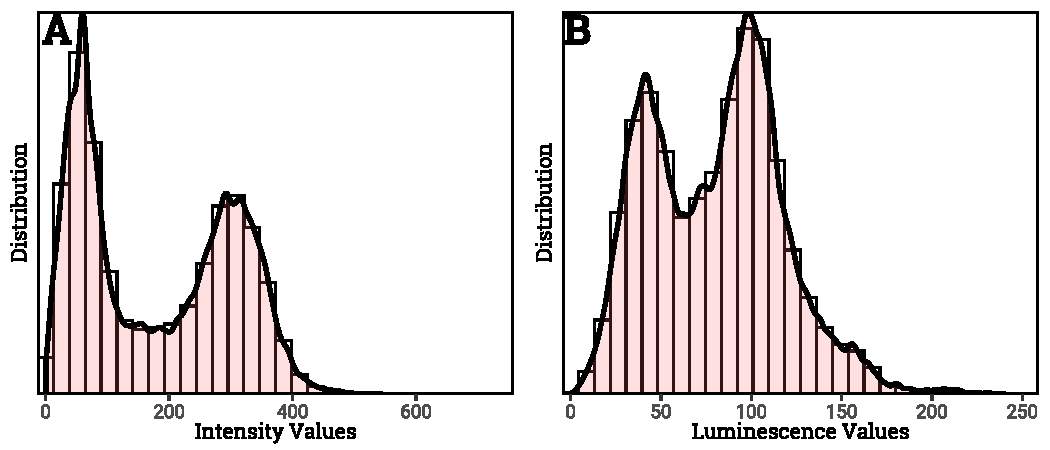
\includegraphics[width=.75\linewidth]{figure/hist_lidar-1} 

}

\caption[Post noise filtering LiDAR point cloud distribution]{Post noise filtering LiDAR point cloud distribution; of \textbf{(A)} Intensity, and \textbf{(B)} Luminescence}\label{fig:hist_lidar}
\end{figure}


\end{knitrout}




\begin{knitrout}\footnotesize
\definecolor{shadecolor}{rgb}{0.969, 0.969, 0.969}\color{fgcolor}\begin{figure}[b]

{\centering 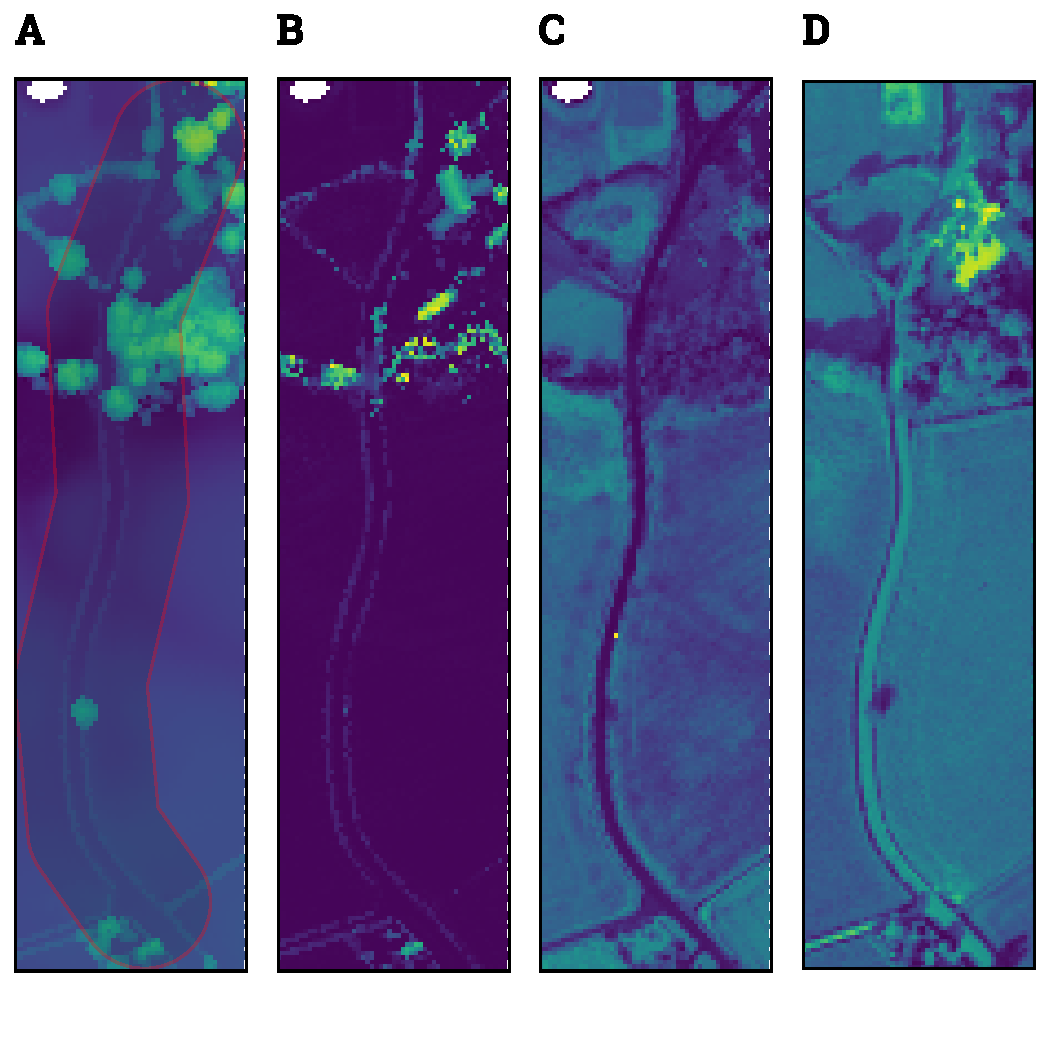
\includegraphics[width=.75\linewidth]{figure/fig_lp-1} 

}

\caption[LiDAR point clouds for one selected road aggregated into 2m$^2$ grids]{LiDAR point clouds for one selected road aggregated into 2m$^2$ grids; \textbf{(A)} Base point cloud $z$ values, road location indicated with a 30m buffer \textbf{(B)} Normalised point cloud $z$ values for only last returns ($lpz$) \textbf{(C)} Normalised point cloud $Intensity$ values for last returns, \textbf{(D)} Aerial data combined to 1 band}\label{fig:fig_lp}
\end{figure}


\end{knitrout}

Following intensity noise filtering, the highest intensity value was now $746$, with a standard deviation of $124$. Figure \ref{fig:hist_lidar} \textbf{(A)} gives the distribution of Intensity values for all points within the study area, showing two clear spikes in intensity, at at value of around 50, with another around 350. This is reflected similarly in the Luminescence values, with two peaks at around 50 and 120 (Figure \ref{fig:hist_lidar} \textbf{(B)}).

Figure \ref{fig:fig_lp} gives the results of further LiDAR preprocessing, comparing Figure \ref{fig:fig_lp} \textbf{(A)} and Figure \ref{fig:fig_lp} \textbf{(B)}, shows how last pulse LiDAR filtering allows for the removal of the majority of tree canopies, leaving only ground points that are considered hard surfaces, and as such are the lowest point the laser pulse has penetrated. Additionally, Figure \ref{fig:fig_lp} \textbf{(B)} shows how a digital terrain model, created through interpolation techniques, using only the base point cloud may be used to normalise the points, giving a digital surface model which only shows the true height of surface objects, without having to consider the variation in lie of the land. However, Figure \ref{fig:fig_lp} \textbf{(C)} indicates that while filtering for last pulse returns may appear to remove much of the canopy, reflected in the $z$ values, the intensity values for points that have penetrated the canopy are lower than those that did not (See the tree just below the centre of the road). This particularly creates issues in the distinction between road and non road in neighbouring areas where the intensity "shadow" created removes the distinct difference in intensity. This suggests that for ground points with multiple returns, the intensity values are likely far less reliable for road classification. Quantitative analysis of this limitation reveals that for ground classified points with a single return the average intensity value is $214.9$, while for ground classified points with multiple returns, the average intensity value is $88.15$.

\section{Perpendicular Sampling}




Using the 30m buffer from known road locations, and sample line extraction, the number of points from the original LiDAR point cloud for the 1km$^2$ area was reduced from $9,419,272$ to $616,015$ giving a reduction in number of points by $93.46$\%. Additionally, including sample lines allowed for filtering based on features of each sample, allowing for samples fully obscured by canopy to be identified through the number of returns, and excluded easily if required. See \textbf{Appendix B}, Figure \ref{fig:sample_fig} for an overview of all the sample lines produced in this analysis.

\section{Linear Probability Model Sensitivity Analysis}

Selected based on literature, and correlation analysis of the variables (See \textbf{Appendix B}, Table \ref{tab:corr}), the first model was constructed to include all variables of importance from the LiDAR point cloud, $z$, Intensity, and Number of Returns. Additionally, luminescence from aerial imagery was included, and the minimum distance of a point from the known road centreline location.


\begin{knitrout}\footnotesize
\definecolor{shadecolor}{rgb}{0.969, 0.969, 0.969}\color{fgcolor}\begin{figure}[tb]

{\centering 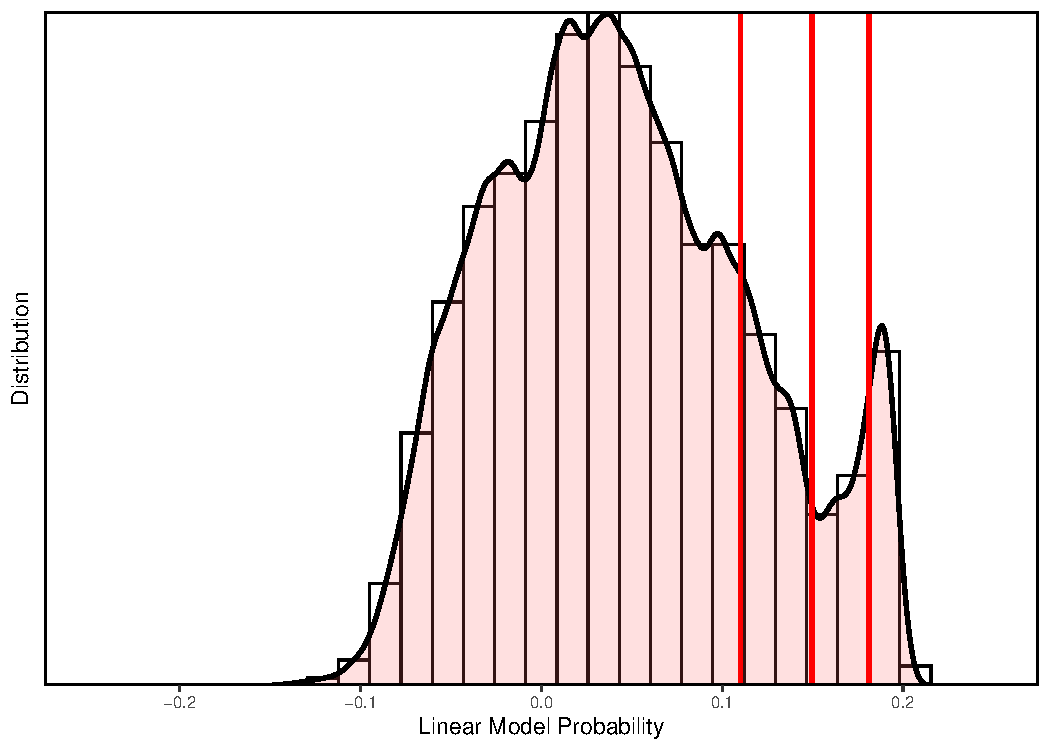
\includegraphics[width=.75\linewidth]{figure/lmdistributions-1} 

}

\caption[Linear model probability distributions for the maximal model (LM 1)]{Linear model probability distributions for the maximal model (LM 1); showing vertical lines at the 95th, 90th, and 80th quantile of the distribution}\label{fig:lmdistributions}
\end{figure}


\end{knitrout}


This first (maximal) model was constructed as;

\begin{equation}
\begin{aligned}
\mathrm{Road}_{t} = \alpha 
    &+ \beta_{1}  \mathrm{Intensity}_{t} \\
    &+ \beta_{2}  \mathrm{Luminescence}_{t}    \\
    &+ \beta_{3}  \mathrm{Z}_{t} \\
    &+ \beta_{4}  \mathrm{NumberOfReturns}_{t} \\
    &+ \beta_{5}  \mathrm{Dist}_{t} + \epsilon
\end{aligned}
\end{equation}

As proposed in Chapter \ref{ch:methods}, Section \ref{sec:lpm}, the road outcome variable was given as points that fell within a 2m buffer of the known road centreline locations. As such, this meant that a fair number of false negative points are expected to have occurred, where points outside 2m of a road centreline location would be incorrectly classified as non-road. Due to this, the classification of non-road and road was not a simple selection of points that were above a 50\% threshold prediction as being road. To determine an appropriate cutoff for road predictions a histogram was produced which gave insight into the distribution of the linear prediction values (Figure \ref{fig:lmdistributions}).


Figure \ref{fig:lmdistributions} shows that there is a clear separation between the majority of points, and higher probability values. This therefore gives insight into the true divide between true road and non-road points, allowing for a qualitative analysis to select the most appropriate quantile of probability values. Three quantiles were chosen, the 95th, 90th and 80th, as indicated on Figure \ref{fig:lmdistributions}. 



\begin{knitrout}\footnotesize
\definecolor{shadecolor}{rgb}{0.969, 0.969, 0.969}\color{fgcolor}\begin{figure}[b]

{\centering 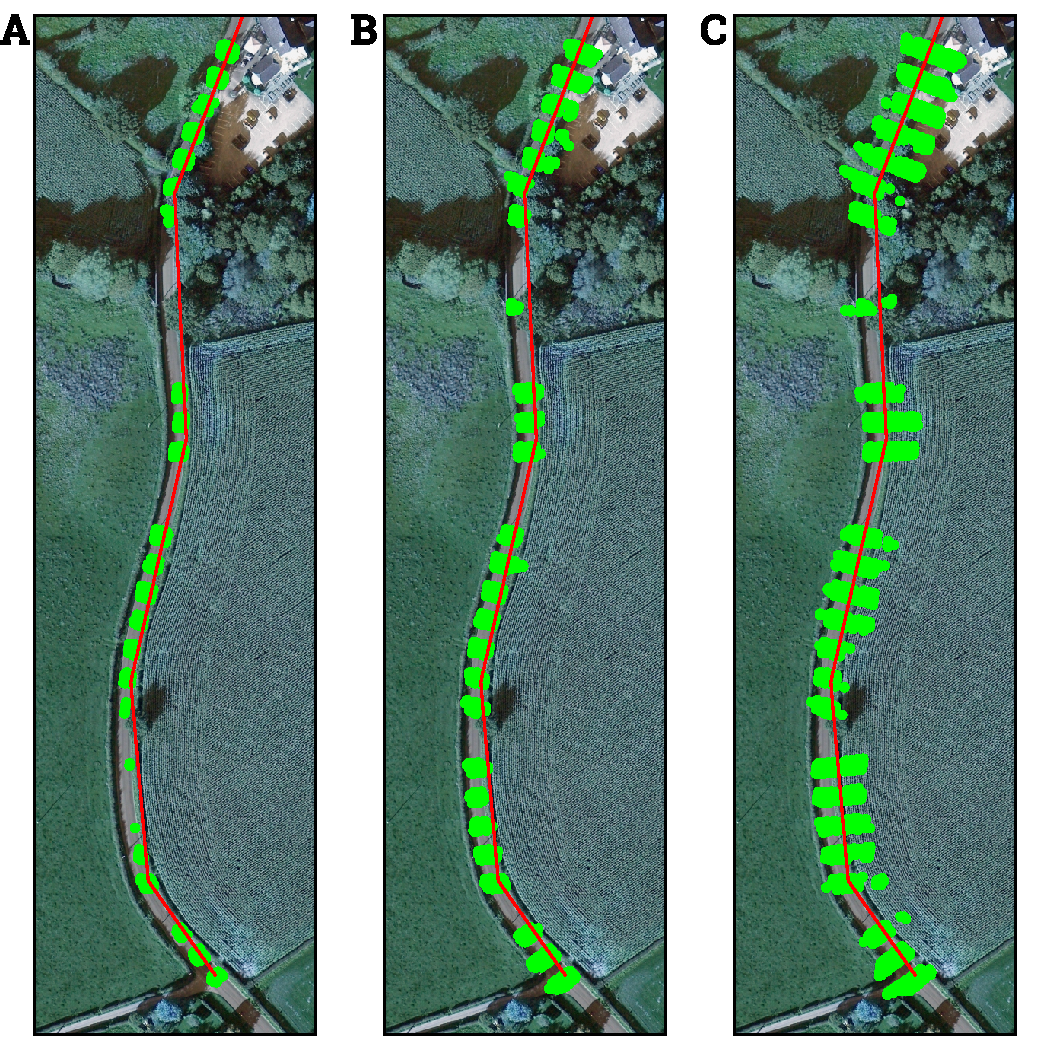
\includegraphics[width=.75\linewidth]{figure/quant_fig-1} 

}

\caption[Comparison between linear prediction quantiles]{Comparison between linear prediction quantiles; \textbf{(A)} 95th quantile, \textbf{(B)} 90th quantile, \textbf{(C)} 80th quantile.}\label{fig:quant_fig}
\end{figure}


\end{knitrout}

Figure \ref{fig:quant_fig} reveals that qualitatively, the optimal choice for a quantile filtering of the linear probability distribution is likely the 95th quantile (Figure \ref{fig:quant_fig} \textbf{(A)}). However, observation of the southern section of Figure \ref{fig:quant_fig} \textbf{(A)} reveals that inaccurate centreline locations have led to an incomplete linear model analysis. To compensate for this, a further method proposed aims to improve the accuracy of the given road centreline locations. Additionally, Figure \ref{fig:quant_fig} \textbf{(A)} reveals that for the 95th quantile probability values, shadow from road hedgerows appears to reduce the model accuracy, as noticeable towards the centre of the road. For this reason, a second model was constructed for later comparison, which removes the $luminescence$ information provided by the aerial imagery;

\begin{equation}
\begin{aligned}
\mathrm{Road}_{t} = \alpha 
    &+ \beta_{1}  \mathrm{Intensity}_{t} \\
    &+ \beta_{2}  \mathrm{Z}_{t} \\
    &+ \beta_{3}  \mathrm{NumberOfReturns}_{t} \\
    &+ \beta_{4}  \mathrm{Dist}_{t} + \epsilon
\end{aligned}
\end{equation}

\section{Corrected Centreline Extraction}

To improve road centreline location accuracy, the 90th quantile results from the first linear probability analysis were used, due to there being a more complete selection of points, but without compromising the true location of roads by including too many outside points.

New road centrelines are given on Figure \ref{fig:fig_noisecent} \textbf{(A)}. Particular improvements are given where the road curves between two open fields, but the original centreline was given as a straight line, covering the hedgerow, and no road surface.





\begin{figure}[b]

{\centering \includegraphics[width=.75\linewidth]{figure/fig_noisecent-1} 

}

\caption[Comparison between original and derived centrelines showing differences in linear models.]{Comparison between original and derived centrelines showing differences in linear models; showing \textbf{(A)} Comparison between original (red) and derived road centrelines (green). \textbf{(B)} Second linear model (LM 2) applied to original centrelines. \textbf{(C)} Second linear model (LM 2) applied to derived centrelines. \textbf{(D)} Individual linear model (LM i) applied to derived centrelines. Each linear model probability quantile is selected as 95\%, green points indicate road classified points, red indicate road classified points, removed through noise isolation filtering.}\label{fig:fig_noisecent}
\end{figure}



Qualitative comparison between the Linear Probability Model based off the original centreline locations reveals an improvement in overall road detection, particularly towards the edge of roads, while additional samples are achieved in areas which previously had no coverage due to the incorrect centreline placement (Figure \ref{fig:fig_noisecent} \textbf{(A)}). However, it appears that in areas where there are higher levels of linear predictive inaccuracy, the new centrelines are less accurate. Thankfully, noise exclusion techniques employed have removed samples that fall within these areas, particularly noticeable at the northern end of Figure \ref{fig:fig_noisecent} \textbf{(C)}. Figure \ref{fig:fig_noisecent} also gives information regarding the distance based noise exclusion technique, which has allowed for the exclusion of isolated points accurately on Figure \ref{fig:fig_noisecent} \textbf{(B)}. Improved centreline locations allowed for individual linear models (Figure \ref{fig:fig_noisecent} \textbf{(D)}). While it was assumed that individual linear models would potentially produce more accurate width estimations, it is hard to differentiate between the global and individual linear models (Figure \ref{fig:fig_noisecent} \textbf{(C)} and \textbf{(D)}).

\section{Final Model Analysis}

For direct comparison between the two selected global linear probability models, centering and scaling of the predictor variables allowed for an easier interpretation of results, without affecting any statistical inferences. This was considered necessary as both $p$ values and standard errors produced by global models offered little in terms of interpretability due to the very large number of points involved in this study. Centering and scaling was obtained through the production of beta coefficients with results given on Table \ref{tab:coeftest}. The removal of luminescence had little effect on the other predictor coefficients, due to the very small influence of this coefficient, reflected by the normalised value (0.01), and the qualitative analysis of the issues due to shadows, as such, it was considered an unnecessary addition. The other coefficients all give insight into their influence of the road outcome, for example for every 1 increase in the standard deviation in $dist$, the likelihood a point is to be a road point decreases by a standard deviation of 0.33. This therefore suggests that the inclusion of the $dist$ coefficient is important, despite not being considered in other supervised road detection techniques.

Table \ref{tab:estwidths} gives a normalised comparison between each linear model, and its associated estimated road width. This gives insight into the effectiveness of various linear probability models for each road, and road type. While average values all give relative accuracy in the region of 70\%, it appears that at present, the method for centreline improvements does not appear to improve road width estimates by much.









\begin{table}[!b]
    \begin{minipage}{.45\linewidth}
    \caption{Model Coefficients, Comparison between Linear Probability Models 1 and 2}\label{tab:coeftest}
      \centering \begin{table}[H]
\centering\begingroup\fontsize{9}{11}\selectfont

\begin{tabular}{lrr}
\toprule
Variable & LM 1 & LM 2\\
\midrule
Intensity & -0.30 & -0.30\\
dists & -0.33 & -0.33\\
Z & -0.07 & -0.07\\
NumberOfReturns & -0.22 & -0.22\\
lum & 0.01 & \\
\bottomrule
\end{tabular}
\endgroup{}
\end{table} \end{minipage}%
    \begin{minipage}{.5\linewidth}
      \centering
    \caption{Comparison between each linear probability model for every road, values given as a percentage in relation to estimated true road width.}\label{tab:estwidths} \begin{table}[H]
\centering\begingroup\fontsize{9}{11}\selectfont

\begin{tabular}{llrrrr}
\toprule
ID & Class & LM $i$ & LM 1 & LM 2 & LM 0\\
\midrule
1 & B Road & 56.74 & 58.60 & 55.79 & 67.23\\
4 & Minor Road & 68.43 & 80.53 & 81.04 & 74.91\\
6 & Minor Road & 69.60 & 74.97 & 70.75 & 69.72\\
7 & B Road & 68.20 & 62.68 & 64.80 & 73.19\\
8 & Minor Road & 73.47 & 60.98 & 73.53 & 74.93\\
9 & Minor Road & 90.83 & 69.29 & 76.83 & 67.54\\
10 & Minor Road & 68.43 & 73.59 & 63.55 & 75.25\\
12 & Minor Road & 99.61 & 96.46 & 86.82 & 88.10\\
13 & B Road & 55.83 & 56.07 & 38.55 & 60.72\\
14 & Local Road & 93.13 & 86.80 & 89.98 & 90.79\\
15 & B Road & 62.97 & 86.13 & 85.44 & 77.03\\
16 & B Road & 55.09 & 65.48 & 56.11 & 69.22\\
18 & Minor Road & 71.65 & 62.30 & 71.61 & 61.76\\
20 & Local Road & 95.01 & 55.85 & 66.93 & 68.56\\
21 & B Road & 67.40 & 60.92 & 75.70 & 71.60\\
30 & Minor Road & 93.79 & 70.82 & 85.19 & 81.11\\
31 & Minor Road & 67.25 & 69.23 & 78.83 & 67.22\\
33 & Minor Road & 68.44 & 70.01 & 64.98 & 73.39\\
34 & Minor Road & 45.01 & 65.44 & 61.68 & 58.40\\
36 & Minor Road & 98.77 & 94.77 & 95.09 & 91.15\\
\hline
\textbf{Means:} & \textbf{} & \textbf{73.48} & \textbf{71.05} & \textbf{72.16} & \textbf{73.09}\\
\bottomrule
\multicolumn{6}{l}{\textsuperscript{} \textbf{LM $i$:} Individual Linear Models}\\
\multicolumn{6}{l}{\textsuperscript{} \textbf{LM 1:} Linear Model inc. lum}\\
\multicolumn{6}{l}{\textsuperscript{} \textbf{LM 2:} Linear Model ex. lum}\\
\multicolumn{6}{l}{\textsuperscript{} \textbf{LM 0:} Linear Model 1 with original road centrelines}\\
\end{tabular}
\endgroup{}
\end{table} \end{minipage} 
\end{table}

\section{Road Assessment}






As LM $i$ gave the highest mean accuracy for roads (Table \ref{tab:estwidths}), it was selected for the final road width predictions. From this, Table \ref{tab:rqi} gives the full results of the road geometric extraction, along with an estimate of overall road quality given by the Road Quality Index (RQI). Qualitative assessment of the RQI may be achieved through observation of the highest and lowest values (Figure \ref{fig:rqi_compare}). It appears to produce reliable results, as the road with the highest RQI is straighter and wider than the road with the lowest RQI, and is likely flat given it is neighboured by houses.

\begin{table}[!h]

\caption{\label{tab:rqi}Overall Features Extracted from Roads in the Study Area, in descending order by RQI value}
\centering
\fontsize{9}{11}\selectfont
\begin{tabular}{llrrrrrr}
\toprule
\textbf{Road ID} & \textbf{Road Function} & \textbf{Max Angle} & \textbf{Total $Z$} & \textbf{Intensity} & \textbf{Width \textbf{(LM $i$)}} & \textbf{Reliability $(\mathbf{P}_{n} / \mathbf{L}$)} & \textbf{RQI}\\
\midrule
21 & B Road & 0.01 & 2.41 & 155 & 3.86 & 2.02 & 0.31\\
15 & B Road & 0.01 & 7.49 & 62 & 3.64 & 0.93 & 0.20\\
9 & Minor Road & 17.15 & 7.31 & 64 & 4.52 & 0.69 & 0.00\\
18 & Minor Road & 9.51 & 3.84 & 101 & 3.63 & 0.46 & -0.03\\
34 & Minor Road & 0.00 & 2.82 & 40 & 2.73 & 14.19 & -0.08\\
16 & B Road & 0.00 & 7.55 & 167 & 3.58 & 1.04 & -0.14\\
20 & Local Road & 0.00 & 1.26 & 319 & 3.68 & 3.90 & -0.19\\
7 & B Road & 0.06 & 7.10 & 299 & 3.78 & 3.83 & -0.40\\
1 & B Road & 0.00 & 3.02 & 281 & 3.15 & 1.26 & -0.47\\
13 & B Road & 0.00 & 3.62 & 313 & 3.35 & 0.74 & -0.47\\
36 & Minor Road & 14.58 & 6.95 & 125 & 3.28 & 0.84 & -0.63\\
30 & Minor Road & 24.53 & 4.93 & 252 & 4.40 & 3.63 & -0.70\\
31 & Minor Road & 10.33 & 11.04 & 251 & 3.50 & 0.53 & -0.95\\
8 & Minor Road & 7.08 & 10.63 & 346 & 3.65 & 0.38 & -1.02\\
4 & Minor Road & 12.81 & 7.29 & 382 & 3.83 & 4.33 & -1.05\\
14 & Local Road & 16.66 & 19.91 & 233 & 4.20 & 0.37 & -1.27\\
10 & Minor Road & 17.95 & 12.08 & 277 & 3.47 & 4.97 & -1.35\\
12 & Minor Road & 18.51 & 15.85 & 370 & 4.66 & 2.03 & -1.35\\
33 & Minor Road & 18.16 & 11.33 & 309 & 3.49 & 4.08 & -1.40\\
6 & Minor Road & 30.38 & 14.03 & 384 & 3.87 & 2.55 & -1.98\\
\bottomrule
\end{tabular}
\end{table}




\begin{knitrout}\footnotesize
\definecolor{shadecolor}{rgb}{0.969, 0.969, 0.969}\color{fgcolor}\begin{figure}[tb]

{\centering 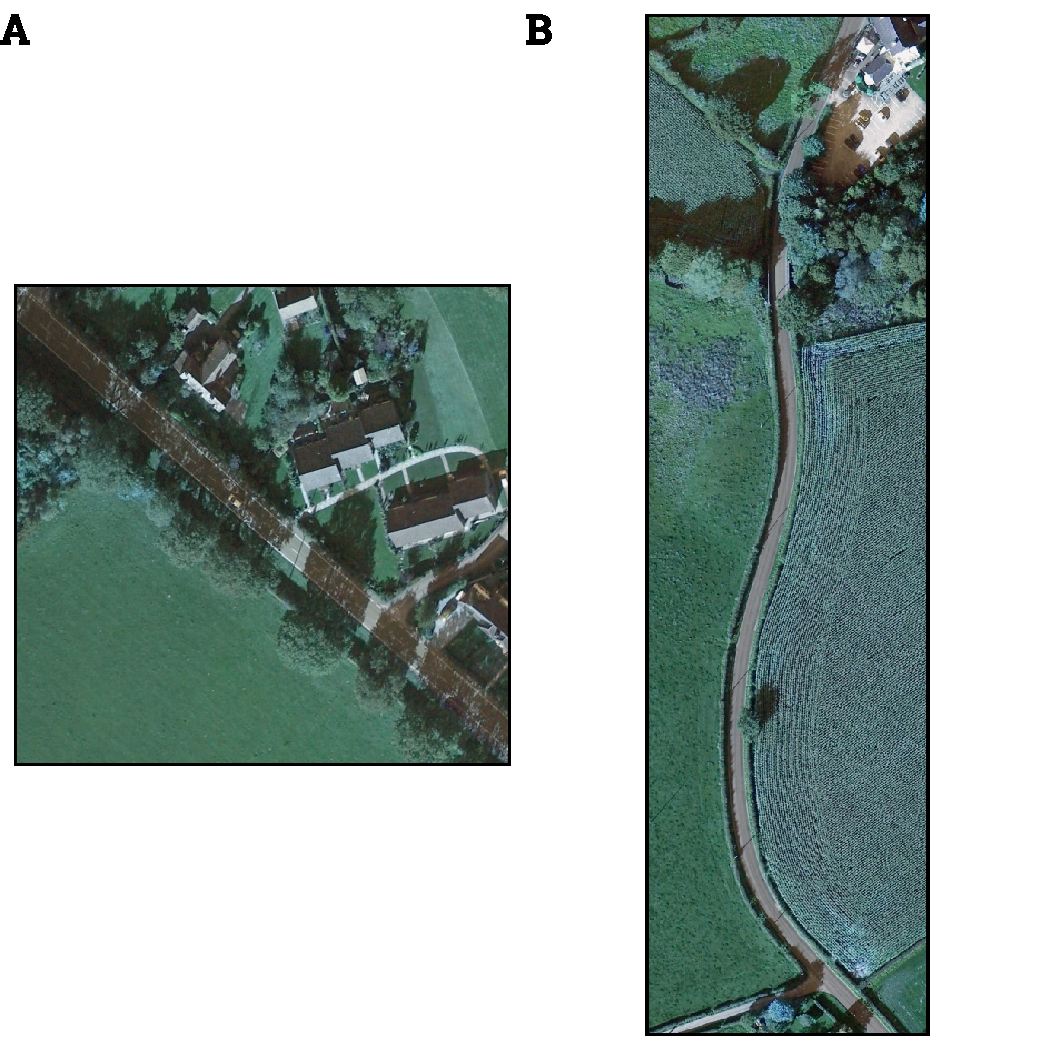
\includegraphics[width=.75\linewidth]{figure/rqi_compare-1} 

}

\caption[Visual comparison between the RQI of roads.]{Visual comparison between the RQI of roads. \textbf{(A)} highest RQI \textbf{(B)} lowest RQI}\label{fig:rqi_compare}
\end{figure}


\end{knitrout}

\chapter{Discussion}
\label{ch:discussion}

\lettrine{T}{he} proposed methodology presents a road classification technique which considers the need for an optimised and efficient extraction of road widths to combine with other road features for use in an automated national rural road assessment. This method builds upon past road classification techniques with the inclusion of Ordinance Survey road centreline geometries allowing for a supervised classification, without the need for the manual and time consuming creation of a training dataset.

While considered to be a supervised method, the training data used in this method is derived from the preexisting OS road centrelines, and as such may be recreated automatically for any road in England, given the comprehensive coverage of this data \citep{ordnancesurvey2019a}. This differs from existing supervised road classification methods, where a training dataset is created and manually labelled \citep[e.g.][]{charaniya2004}. Additionally, the majority of LiDAR road classification techniques focus on unsupervised methods \citep[e.g.][]{clode2004,vosselman2009,jaakkola2008,darmawati2008}, and as such do not consider the use of any training data, with the primary goal of obtaining accurate road locations. Such techniques often limit their scope to road centreline extraction which has a limited use case with a preexisting national road centreline database. Notably, \cite{zhang2018} assess the accuracy of their technique by comparing derived road centrelines to an existing road centreline database which renders little in terms of practical application.

Therefore, the method presented in this dissertation considers a more practical approach, providing an intermediate between unsupervised and supervised methods, which integrates the known road centrelines into the road classification. Rather than attempting to classify road centrelines, or the full road surface, this dissertation concentrates on the requirement for road feature extraction as presented in various UK government rural road studies \citep{departmentfortransport2018b,departmentfortransport2013a,roadsafetyandenvironment2000}.  With the primary focus of road classification on the automated road width extraction. Focusing on solely width extraction enables road surface sampling, primarily enabling a reduction in computational overhead, while adding the benefit of more simplistic noise filtering techniques, and a per road width classification.

\section{Effectiveness of the Method}
\subsection{Computational Efficiency}

Direct comparison between the computational efficiency of this method and past methods is not possible due to the unique data used in this study. However, \cite{zhang2016} outline some specifications of the dataset used in their supervised road centreline extraction using LiDAR and aerial imagery. With aerial imagery at a resolution of 15cm, and a total 5200 by 5000 pixels, the study area therefore covers 780m by 750m. Similar to the 1km$^2$ for this study. The total time taken for object extraction for this area in their method was 37.87 minutes, compared with the 16.2 minutes proposed in this paper. It is expected that the method proposed by \cite{zhang2016} should take far longer to compute due to being the inclusion of complex methodologies such as image segmentation through random forest classification, and without any preliminary removal of LiDAR points such as the 30m buffer from known road centrelines used in this dissertation.

\subsection{Comparison with Similar Studies}

Despite several road classification methodologies proposing the inclusion of aerial imagery to assist with accuracy \citep[e.g.][]{charaniya2004,hui2008,guan2013}, this study reveals that for roads overlooked by tall features such as hedgerows, the shadow created reduces overall classification accuracy. Additionally, the inclusion of aerial data provided little benefit in areas without shadows, likely due to the more distinct separation in intensity values from a rural road surface and surrounding vegetation, unlike that found in a more urban setting. 

Due to the irregularity of LiDAR and the large number of points, many past road classification techniques have relied on regulating the data into a grid \citep{hatger2005}. For example, \cite{clode2004} used LiDAR with a resolution of 0.8m, and regularised this into a grid to produce a DTM and subsequently extract road centrelines. Due to this aggregation, they were able to filter points through a density threshold, and produce road centrelines. However, using this method to find road widths proved more difficult, and as \cite{hatger2005} note; the function that derived road widths in this paper resulted in some ambiguity.

The focus of many road classification techniques are primarily directed towards either centreline extraction \citep{clode2004,zhang2018,matkan2014}, or the use of ground based LiDAR for use in automated vehicles \citep{jaakkola2008,yoon2009}, and almost all studies appear to focus on urban road classification \citep{li2016,vosselman2009,zhao2012}, while even studies considering "rural" areas, do not represent roads that would be found in the context of rural England \citep{azizi2014,mena2005}, and exclude key features such as hedgerows, overhanging vegetation, with the road surface appearing fully distinct from neighbouring verges. Additionally these studies do not focus primarily on road width extraction, and as such are limited by the requirement for the inclusion of all points of data, to obtain a full road extraction.

The study of the speed accident relationship on rural British roads by \cite{taylor2002} outlined some techniques for the extraction of rural British road features, and as such was able to begin an assessment for the classification of rural road hierarchies. However, the data collection technique employed included drive-through video recordings, not allowing for a scalable approach. Results also often lacked in accuracy, taking the road height variation from OS 10m contour lines. The method proposed in this dissertation aims to alleviate these problems by ensuring a higher level of accuracy in height variation, through the use of LiDAR data with a +/-25cm RMSE. As well as allowing for a computational technique that does not rely on the manual collection of ground-based data, and instead uses aerial LiDAR which is more practically feasible to obtain for a comprehensive study. LiDAR has multiple use cases, meaning the national production of this data is well funded.

\section{Applications of this Methodology}
\subsection{Stopping Sight Distance}

Stopping Sight Distances are an important consideration for rural British roads. From qualitative observation of aerial imagery, and personal knowledge, hedgerows that bank the verges either side of many rural British roads often fully obscure the sight line around sharp bends, meaning it is often impossible to see oncoming traffic or obstacles, which, given the nature of these roads can often be large farm vehicles which spill into multiple lanes, or hazards such as farm animals, or unsafe road conditions. It is worth mentioning that the majority of hedgerows have automatic protection under the Hedgerow Regulations 1997 \citep{ukgovernment1997} for numerous historic and environmental reasons \citep[e.g. protected species;][]{ukgovernment1981}, as such, their removal for road safety is rarely granted.

Stopping Sight Distance is defined as the ability to see an object in the roadway with enough distance to stop, Table \ref{tab:ssd} outlines the calculated stopping sight distances at certain speeds, giving a rough indication of the distance required between a car and bend in a road. For example, Table \ref{tab:ssd} indicates that at 100kph (60mph), stopping sight distance is recommended to be 185m. Broadly, for a road to be considered appropriate for a 60mph limit, it could be said that it should not have a bend which impairs the line of sight within 185m such a speed limit. For a rough idea of the number of bends per road (ignoring bend sharpness), there is an additional table given in \textbf{Appendix B}, Table \ref{tab:rd_bends}.

Assumptions for certain road regulations are made that drivers will slow to appropriate speeds to adapt to road conditions, either in poor weather, or to approach a sharp bend, however \cite{layton2012} note that often this is not that case, and drivers often do not slow appreciably to account for these conditions. Therefore suggesting that speed limits should more accurately reflect the conditions of the road. Additionally, stopping sight distances observed by \cite{layton2012} are significantly longer for larger vehicles such as trucks, and given the large farm vehicles often present on country roads, speed policy should take this into account.

\begin{table}[b]
\centering
\fontsize{9}{10}\selectfont
\caption{Recommended minimum Stopping Sight Distances at certain speeds \citep{layton2012}}
\label{tab:ssd}
\begin{tabular}{lcccc}
\toprule
\textbf{Speed} &
\multicolumn{2}{l}{\textbf{Stopping Sight Distance}} &
\multicolumn{2}{l}{\textbf{Typical Emergency Stopping Distance (m)}} \\ 
\midrule
Design Speed &
Calculated &
Design &
Wet Pavement &
Dry Pavement \\
(km/h) &
(2.5$^s$, a=3.4m/s$^2$) &
(2.5$^s$, a) &
(1$^s$, f$_{wet}$) &
(1$^s$, f$_{dry}$) \\
\midrule
30 & 31.2 & 35 & 17.1 & 14.2 \\
40 & 46.2 & 50 & 27.7 & 21.6 \\
50 & 63.5 & 65 & 42.0 & 30.3 \\
60 & 83.0 & 85 & 59.6 & 40.3 \\
70 & 104.9 & 105 & 81.7 & 51.6 \\
80 & 129.0 & 130 & 106.1 & 64.2 \\
90 & 155.5 & 160 & 131.2 & 78.1 \\
100 & 184.2 & 185 & 163.4 & 93.4 \\
110 & 215.3 & 220 & 200.6 & 110.0 \\
120 & 248.6 & 250 & 235.7 & 127.9 \\
 \bottomrule
\end{tabular}
\end{table}

Road features extracted in this dissertation may be used to inform the current likely stopping sight distances, combining key features such as the width of roads, which influences the sight line, the max bend angle within a road segment, and the elevation change.

\subsection{Improving Rural Transport Accessibility}

Transport disadvantage is a key limitation of transport accessibility, that may be due to lack of public transport, a poor road network, or a persons physical inability to reach a destination due to disability \citep{smith2012}. Often transport disadvantage may be alleviated through access to public transport, as this removes the requirement for private transport ownership, limited by both income and ability to drive. However, public transport in rural areas is often limited or absent, meaning rural transport predominantly relies on private road vehicles, limiting access for those who are unable to drive, such as children, the elderly, and people with disabilities \citep{manthorpe2008}. Additionally, this reliance on private transport increases the minimum cost of living in rural communities, given car ownership is often considered mandatory but often isn't taken into account when assessing the minimum cost of living in rural areas \citep{smith2012}. For those who are unable to access private transport, accessibility is considered limited through capability, rather than pure accessibility through journey times and other factors \citep{currie2010}. Rural areas in particular often have larger elderly populations, meaning capability is often a key issue in areas with poor public transport, and can lead to social exclusion for those without cars \citep{solomon2009}.

Transport accessibility is defined by the UK Government through journey time estimates for populations to particular key services. In particular, the UK Government uses official accessibility indicators to set minimum thresholds for journey time access to education, health services, employment and retail hubs \citep{departmentfortransport2016}, also taking into account the availability of public transport services. Accessibility in rural areas is found to be far poorer than urban areas based off minimum travel times to various services, and while travel by car generally reduces travel times, the rate is still far below urban areas. This journey time data is simplified, giving the start point of journeys as a single point within Output Area census units, and aggregated road speeds. The output of this data is given at the LSOA level which is then used for accessibility analysis. Journey times are obtained through mass collection of GPS data by INRIX \citep{inrix2019} which is then used in TRACC software \citep{tracc2019}.

Due to the limited use of rural roads, the GPS data obtained for speed estimates are likely far less reliable than for urban areas. Additionally, calculating journey time in rural areas should consider the road geometry, which the above method ignores. By considering features such as road width, quality, bends, and elevation change, the suitability of certain roads for particular vehicle types may be informed. For example, rural healthcare accessibility is becoming more of an issue given fewer healthcare professionals now live in rural communities, \citep{farmer2003}, and the urban centralisation of hospital services \citep{mungall2005} means that understanding the level of access that each rural community has to these services is more important than ever. Emergency vehicles are often far larger than personal transportation, meaning GPS times derived from smaller personal transportation likely does not provide an accurate journey time estimate for these vehicle types, as the geometric features of certain roads likely do not allow for these vehicles. Aggregation and simplification of journey time estimates also do not provide a comprehensive estimate of the true journey times for each rural road, which would be achievable through the road feature extraction presented in this dissertation. The individual rural road features may provide further insight into specific roads which require targeted improvements to alleviate accessibility problems, without suffering from inherent geographical limitations such as the MAUP \citep{openshaw1984a}, imposed by journey time aggregation.

\subsection{New Forms of Public Transport}

There is a strong urban bias for the development of new transport technologies \citep{malecki2003}, explained through key issues particular to rural transport systems;

\begin{itemize}
    \item \textbf{Service area:} Rural transport agencies often serve large areas with long trips. As a result, assisting passengers needs is not easy and attending immediately to a problem that arises on the road is difficult (e.g. rescheduling trips when an incident occurs.)
    \item \textbf{Service Coordination:} There are different basic public services e.g. healthcare and education with overlapping areas of services. It is challenging to coordinate services and resources among the agencies and other providers.
    \item \textbf{Infrastructure:} Rural areas suffer a lack of communication infrastructure e.g. wireless communications services, real-time communication from and to rural passengers.
    \item \textbf{Fleet size:} Although tech can solve several transportation problems in remote rural areas, it might be difficult to fund and develop at a small scale.
\begin{flushright}
    \footnotesize{\citep{riva2011}}
\end{flushright}
\end{itemize}

While it may appear that many of these issues are inherent to rural areas, and unsolvable, the optimisation of transport technologies for rural areas may be made more achievable through access to the comprehensive road data provided through the methods proposed in this dissertation. \cite{palmer2004} state that flexible integrated transport services are a likely public transport implementation that would benefit rural areas without the limitations outlined above, such a technology would rely extensively on a full understanding of the road network on which it would be dispatched. The \cite{departmentfortransport2016} call for "Unconventional modes" of public transport in such areas, building mainly on a bottom up approach to meet direct demand. Additionally, vehicles supplied through such an implementation would account for suitability to both road conditions and consumer demand, allowing for vehicles smaller than a typical bus for example on narrower roads \citep{mulley2009}. There is also a significant call for the inclusion of a more comprehensive understanding of the road network through advanced computational techniques to improve the efficiency and quality of existing transport systems \citep{deeter2009}, including a more flexible transport management system \citep{robinson2008}.

\subsection{Other Applications}

Supply chains rely on a well maintained road infrastructure, and as such, many rural areas are considered to be (economically) "Lagging Rural Regions", due to their geographical remoteness, poor infrastructures, low population density and limited employment opportunities, often supported economically by an agricultural backbone \citep{ilbery2004}. Improving the economy of such areas therefore relies primarily on the effectiveness of the supply chains, often limited due to the poor infrastructures \citep{marsden2002}, and recent demand for large scale supply chains is limited in these areas due to the overall quality of the road network. To further understand the limitations of rural supply chains inherently relies on a full understanding of the road network, whether to acknowledge where limitations exist, or to develop opportunities for optimisation of the supply chains. Similarly, \cite{bosona2011} call for location analysis of supply chains through quantifiable data, to better optimise supply routes.

\section{Current Limitations of this Method}


As results have revealed, it is relatively hard to quantify the accuracy of this particular linear probability analysis, and often the accuracy has been assessed qualitatively. The ultimate goal with this method would be to produce a model which may be assessed quantitatively, allowing for a more conclusive and full automation. It should also be noted that the quantile selection at present is based on a qualitative observation of the distribution of linear probability values for the current 1km$^2$ area, and as such it would be essential to find a method to quantitatively assess the cutoff for road and non-road points in order for this method to be used with other roads.

At present the removal of noise at the final stage of the road classification comes from both identifying isolated points (See Function \ref{code:max_lines}), and the removal of calculated widths that are above 8m and below 2m (See \textbf{Appendix \ref{c:script}}). While logically it makes sense to include limitations for widths, given a road below 2m would not support even single way traffic, and a 8m road is unexpected for any rural single carriageway, these limitations are still arbitrary, and for all unclassified roads in England, there is no minimum width required \citep{highwaysengland2016}.

Alternatives to Linear Probability models do exist when considering binary outcome variables, one being probabilistic regression, which takes the cumulative standard normal distribution function ($\Phi$) to model the regression. Interpretability of results may be aided through this method as it includes consideration of the quantiles associated with a unit change in outcome variables. Additionally logistic (and probabilistic) regression, unlike simple linear regression do not take the assumption that there is a linear distribution in the outcome, weighting values more towards 1 or 0, conforming more with the distribution of a binary outcome variable \citep[See Figure \ref{fig:csnd};][]{hanck2019}. However, preliminary analysis of the methodology in this study did consider a logistic regression, but found that interpretability of the quantiles and results was difficult, and qualitative observation of the results did not appear to provide much benefit over linear regression.

\begin{figure}[t]
    \centering
\begin{tikzpicture}[scale=1]
\tikzset{
    declare function={
        normcdf(\x,\m,\s)=1/(1 + exp(-0.07056*((\x-\m)/\s)^3 - 1.5976*(\x-\m)/\s));
    }
}
\begin{axis}[%
  grid=major]
  \addplot[mark=none, red!50] coordinates {(-6,0) (6,1)};
  \addplot [smooth, black] {normcdf(x,0,2)};
\end{axis}
\end{tikzpicture}
\caption{Comparison between a Linear Probability Model Distribution (Red) and Probit/Logit Cumulative Standard Normal Distribution (Black) \citep[Approximation credit][]{bowling2009})}\label{fig:csnd}
\end{figure}

Alternative methods to reduce the noise produced in road classification may include the identifications of straight line road edges, a distinguishing feature of man made structures \cite{guan2013}. This could enable point exclusion if outside of a particular threshold in relation to other points. LiDAR classification techniques often make use of segmentation algorithms to identify objects from geometric features such as planes, and straight edges \citep{wang2009}. These include Hough transforms \citep{vosselman2004,clode2004}, RANSAC \citep{smadja2010,sampath2008}, and least square fitting \citep{matkan2014}.

Additionally, unsupervised LiDAR classification techniques have considered the texture of road and non-road, where man made structures often have smooth, regular height textures, and small height variations, while trees and other vegetation give an irregular height pattern,  using this to separate man made structures, such as roads, from vegetation \citep{vosselman2004,darmawati2008}.

Driving behaviour is affected by particular features that are not covered in this methodology, namely the delineation of road centrelines and edges \citep{steyvers2000,charlton2018}. The detection of these features is influenced  by either if a road edge is easily detectable, or if a road has painted markings to indicate a centreline, both of which are not observable through this methodology, and would likely rely on mobile LiDAR data collection.

\section{Conclusion}

This dissertation presents a methodology for the extraction of road features to enable a fuller understanding of the rural British road network. The method presented considers the requirement for supervised classification of roads to determine road width, that utilises existing OS open road data which is freely available. Concentrating on the practical applications of determining road width enables the use of a sampling classification, which reduces computational load, and enables sample based filtering.

Results generally provide insight into the overall road quality of individual roads in relation to each other, but work is required to more accurately extract key features in road quality assessment, particularly road widths. Further development of this method would provide road features for use in a national assessment of rural roads in Britain, to aid with improvements with the understanding of rural accessibility, the response time of emergency services, more appropriate speed limits, and rural road hierarchies.

% ===========================================================================================================
% Bibliography
% ===========================================================================================================

\bibliographystyle{jss}
\linespread{1}
\bibliography{kbib, rbib}


\begin{center}
% remember to compile twice for current word count
Word Count: 11986

\end{center}

\cleardoublepage

% ===========================================================================================================
% Appendices
% ===========================================================================================================
\appendix
\chapter{Environment and Functions}
\label{a:code}

    All code is hosted on my personal \href{https://github.com/cjber/}{GitHub account}, along with my complete dotfiles, used in conjunction with the Linux distribution Manjaro, and the i3 window manager. All writing and code was produced using \href{https://neovim.io}{Neovim} with my personal configuration to implement integrated development environment (IDE) style features for writing R code, while also providing essential features for writing in \LaTeX{}. Neovim has the benefit of being both highly customisable, and lightweight, which allows for much lower system utilisation compared with R Studio when working with large datasets. One essential Vim plugin to mention is \href{https://github.com/jalvesaq/Nvim-R}{Nvim-R}, providing an \R{} REPL connection to vim, and other useful functions. 

This dissertation was written using \LaTeX{} combined with the \texttt{rnoweb} file type \citep{ihaka2011}, for \textit{Literate Programming}\footnote{See \cite{knuth1984}; \textit{“Let us change our traditional attitude to the construction of programs: Instead of imagining that our main task is to instruct a computer what to do, let us concentrate rather on explaining to human beings what we want a computer to do.”}}. The template is built from scratch but takes much inspiration (and code) from the \href{https://github.com/asardaes/R-LaTeX-Template}{R-LaTeX-Template}.

\section{Packages and Machine Environment}


\begin{knitrout}\footnotesize
\definecolor{shadecolor}{rgb}{0.969, 0.969, 0.969}\color{fgcolor}\begin{kframe}
\begin{verbatim}
Machine:     
[1] "AMD Ryzen 5 2600 Six-Core Processor"
Num cores:   
[1] 12
Num threads: 
[1] 12
RAM:         
33.7 GB
\end{verbatim}
\end{kframe}
\begin{kframe}\begin{verbatim}
R version 3.6.1 (2019-07-05)
Platform: x86_64-pc-linux-gnu (64-bit)
Running under: Manjaro Linux

Matrix products: default
BLAS:   /usr/lib/libopenblasp-r0.3.6.so
LAPACK: /usr/lib/liblapack.so.3.8.0

attached base packages:
[1] parallel  stats     graphics  grDevices utils     datasets  methods  
[8] base     

other attached packages:
 [1] wesanderson_0.3.6          data.table_1.12.2         
 [3] showtext_0.7               showtextdb_2.0            
 [5] sysfonts_0.8               benchmarkme_1.0.2         
 [7] bibtex_0.4.2               cowplot_1.0.0             
 [9] pbapply_1.4-2              rgdal_1.4-4               
[11] future_1.14.0              varhandle_2.0.3           
[13] forcats_0.4.0              stringr_1.4.0             
[15] dplyr_0.8.3                purrr_0.3.2               
[17] readr_1.3.1                tidyr_0.8.3               
[19] tibble_2.1.3               tidyverse_1.2.1           
[21] lidR_2.1.2                 raster_3.0-2              
[23] sp_1.3-1                   scales_1.0.0              
[25] kableExtra_1.1.0           sf_0.7-7                  
[27] ggpubr_0.2.3               magrittr_1.5              
[29] viridis_0.5.1              viridisLite_0.3.0         
[31] broom_0.5.2                RStoolbox_0.2.6           
[33] ggthemes_4.2.0             PerformanceAnalytics_1.5.3
[35] xts_0.11-2                 zoo_1.8-6                 
[37] Hmisc_4.2-0                Formula_1.2-3             
[39] survival_2.44-1.1          lattice_0.20-38           
[41] devtools_2.2.0             usethis_1.5.1             
[43] ENVS450_0.1.0              ggplot2_3.2.1             
[45] pacman_0.5.1               knitr_1.24                
[47] nvimcom_0.9-83             colorout_1.2-1            
\end{verbatim}
\end{kframe}
\end{knitrout}
\newpage

\section{Referenced Functions}
\subsection{LiDAR Clean} \label{code:lidr_clean}
\begin{knitrout}\footnotesize
\definecolor{shadecolor}{rgb}{0.969, 0.969, 0.969}\color{fgcolor}\begin{kframe}
\begin{alltt}
\hlstd{lidr_clean} \hlkwb{<-} \hlkwa{function}\hlstd{(}\hlkwc{cluster}\hlstd{) \{}
  \hlstd{las} \hlkwb{<-} \hlkwd{readLAS}\hlstd{(cluster)}
  \hlkwa{if} \hlstd{(}\hlkwd{is.empty}\hlstd{(las)) \{}
    \hlkwd{return}\hlstd{(}\hlkwa{NULL}\hlstd{)}
  \hlstd{\}}
  \hlcom{# remove all but last return}
  \hlstd{las} \hlkwb{<-} \hlkwd{lasfilter}\hlstd{(las, NumberOfReturns} \hlopt{==} \hlstd{ReturnNumber)}

  \hlcom{# find ground points}
  \hlstd{las} \hlkwb{<-} \hlkwd{lasground}\hlstd{(las,} \hlkwd{csf}\hlstd{())}

  \hlcom{## Create Point DEM}
  \hlcom{# interpolate ground points to create raster dtm. Uses Classification = 2}
  \hlcom{# very large number of points, therefore idw used as opposed to kriging}
  \hlstd{dtm} \hlkwb{<-} \hlkwd{grid_terrain}\hlstd{(las,} \hlnum{1}\hlstd{,} \hlkwd{knnidw}\hlstd{(}\hlkwc{k} \hlstd{=} \hlnum{10}\hlstd{,} \hlkwc{p} \hlstd{=} \hlnum{2}\hlstd{))}
  \hlcom{# normalise heights using dtm}
  \hlstd{las} \hlkwb{<-} \hlkwd{lasnormalize}\hlstd{(las, dtm)}
  \hlkwd{return}\hlstd{(las)}
\hlstd{\}}
\end{alltt}
\end{kframe}
\end{knitrout}
\subsection{Extract Buffer} \label{code:extract_buff}
\begin{knitrout}\footnotesize
\definecolor{shadecolor}{rgb}{0.969, 0.969, 0.969}\color{fgcolor}\begin{kframe}
\begin{alltt}
\hlstd{extract_buff} \hlkwb{<-} \hlkwa{function}\hlstd{(}\hlkwc{cluster}\hlstd{,} \hlkwc{clip_input}\hlstd{) \{}
  \hlstd{las} \hlkwb{<-} \hlkwd{readLAS}\hlstd{(cluster)}

  \hlkwa{if} \hlstd{(}\hlkwd{is.empty}\hlstd{(las)) \{}
    \hlkwd{return}\hlstd{(}\hlkwa{NULL}\hlstd{)}
  \hlstd{\}}

  \hlcom{# ensure no null input}
  \hlkwa{if} \hlstd{(}\hlopt{!}\hlkwd{is.null}\hlstd{(clip_input)) \{}
    \hlstd{las} \hlkwb{<-} \hlkwd{lasclip}\hlstd{(las, clip_input)}

    \hlcom{# bind clipped inputs together}
    \hlcom{# as gives list depending on number of}
    \hlcom{# sp objects}
    \hlkwa{if} \hlstd{(}\hlkwd{length}\hlstd{(las)} \hlopt{>} \hlnum{1}\hlstd{) \{}
      \hlkwa{for} \hlstd{(i} \hlkwa{in} \hlnum{1}\hlopt{:}\hlkwd{length}\hlstd{(las)) \{}
        \hlkwa{if} \hlstd{(}\hlopt{!}\hlkwd{is.empty}\hlstd{(las[[i]])) \{}
          \hlstd{las} \hlkwb{<-} \hlkwd{do.call}\hlstd{(rbind, las)}
          \hlkwd{return}\hlstd{(las)}
        \hlstd{\}}
      \hlstd{\}}
    \hlstd{\}}
  \hlstd{\}}
\hlstd{\}}
\end{alltt}
\end{kframe}
\end{knitrout}
\subsection{Filter LAS Noise} \label{code:las_filter_noise}
\begin{knitrout}\footnotesize
\definecolor{shadecolor}{rgb}{0.969, 0.969, 0.969}\color{fgcolor}\begin{kframe}
\begin{alltt}
\hlstd{las_filter_noise} \hlkwb{<-} \hlkwa{function}\hlstd{(}\hlkwc{cluster}\hlstd{,} \hlkwc{sensitivity} \hlstd{=} \hlnum{1}\hlstd{) \{}
  \hlstd{las} \hlkwb{<-} \hlkwd{readLAS}\hlstd{(cluster)}
  \hlkwa{if} \hlstd{(}\hlkwd{is.empty}\hlstd{(las)) \{}
    \hlkwd{return}\hlstd{(}\hlkwa{NULL}\hlstd{)}
  \hlstd{\}}
  \hlcom{# find 95th quantile intensity values per 10m^2}
  \hlstd{p95i} \hlkwb{<-} \hlkwd{grid_metrics}\hlstd{(las,} \hlopt{~} \hlkwd{quantile}\hlstd{(Intensity,} \hlkwc{probs} \hlstd{=} \hlnum{0.95}\hlstd{),} \hlnum{10}\hlstd{)}
  \hlstd{p95z} \hlkwb{<-} \hlkwd{grid_metrics}\hlstd{(las,} \hlopt{~} \hlkwd{quantile}\hlstd{(Z,} \hlkwc{probs} \hlstd{=} \hlnum{0.95}\hlstd{),} \hlnum{10}\hlstd{)}
  \hlcom{# join by merging}
  \hlstd{las} \hlkwb{<-} \hlkwd{lasmergespatial}\hlstd{(las, p95i,} \hlstr{"p95i"}\hlstd{)}
  \hlcom{# remove above 95th quantile}
  \hlstd{las} \hlkwb{<-} \hlkwd{lasfilter}\hlstd{(las, Intensity} \hlopt{<} \hlstd{p95i} \hlopt{*} \hlstd{sensitivity)}

  \hlstd{las} \hlkwb{<-} \hlkwd{lasmergespatial}\hlstd{(las, p95z,} \hlstr{"p95z"}\hlstd{)}
  \hlcom{# remove above 95th quantile}
  \hlstd{las} \hlkwb{<-} \hlkwd{lasfilter}\hlstd{(las, Z} \hlopt{<} \hlstd{p95z} \hlopt{*} \hlstd{sensitivity)}
  \hlcom{# remove unneeded var}
  \hlstd{las}\hlopt{$}\hlstd{p95i} \hlkwb{<-} \hlkwa{NULL}
  \hlstd{las}\hlopt{$}\hlstd{p95z} \hlkwb{<-} \hlkwa{NULL}
  \hlkwd{return}\hlstd{(las)}
\hlstd{\}}
\end{alltt}
\end{kframe}
\end{knitrout}

\subsection{Combine Catalog} \label{code:comb_ctg}
\begin{knitrout}\footnotesize
\definecolor{shadecolor}{rgb}{0.969, 0.969, 0.969}\color{fgcolor}\begin{kframe}
\begin{alltt}
\hlstd{comb_ctg} \hlkwb{<-} \hlkwa{function}\hlstd{(}\hlkwc{x}\hlstd{) \{}
  \hlstd{las} \hlkwb{<-} \hlkwd{readLAS}\hlstd{(x)}
  \hlkwa{if} \hlstd{(}\hlkwd{is.empty}\hlstd{(las)) \{}
    \hlkwd{return}\hlstd{(}\hlkwa{NULL}\hlstd{)}
  \hlstd{\}}
  \hlkwd{return}\hlstd{(las)}
\hlstd{\}}
\end{alltt}
\end{kframe}
\end{knitrout}

\subsection{Road Angles}\label{code:road_angles}
\begin{knitrout}\footnotesize
\definecolor{shadecolor}{rgb}{0.969, 0.969, 0.969}\color{fgcolor}\begin{kframe}
\begin{alltt}
\hlcom{# atan2 to find angle between two centreline segments}
\hlcom{# relative to previous centreline orientation}
\hlstd{road_angles} \hlkwb{<-} \hlkwa{function}\hlstd{(}\hlkwc{rd}\hlstd{) \{}
  \hlstd{coords} \hlkwb{<-} \hlstd{rd} \hlopt \hlkwd{st_coordinates}\hlstd{()}
  \hlstd{angle} \hlkwb{<-} \hlkwd{c}\hlstd{()}
  \hlkwa{if} \hlstd{(}\hlkwd{nrow}\hlstd{(coords)} \hlopt{>} \hlnum{1}\hlstd{) \{}
    \hlkwa{for} \hlstd{(i} \hlkwa{in} \hlnum{1}\hlopt{:}\hlstd{(}\hlkwd{nrow}\hlstd{(rd)} \hlopt{-} \hlnum{1}\hlstd{)) \{}
      \hlstd{n1} \hlkwb{<-} \hlstd{coords[i, ]}
      \hlstd{n2} \hlkwb{<-} \hlstd{coords[i} \hlopt{+} \hlnum{1}\hlstd{, ]}
      \hlstd{x} \hlkwb{<-} \hlstd{n1[}\hlnum{1}\hlstd{]} \hlopt{-} \hlstd{n2[}\hlnum{1}\hlstd{]}
      \hlstd{y} \hlkwb{<-} \hlstd{n1[}\hlnum{2}\hlstd{]} \hlopt{-} \hlstd{n2[}\hlnum{2}\hlstd{]}
      \hlstd{ang_rad} \hlkwb{<-} \hlkwd{atan2}\hlstd{(y, x)}
      \hlstd{ang_deg} \hlkwb{<-} \hlstd{ang_rad} \hlopt{/} \hlstd{pi} \hlopt{*} \hlnum{180}

      \hlstd{angle} \hlkwb{<-} \hlkwd{append}\hlstd{(angle, ang_deg)}
      \hlcom{# left of N same as right of N}
      \hlcom{# same as + 2pi}
      \hlstd{angle} \hlkwb{<-} \hlkwd{abs}\hlstd{(angle)}
    \hlstd{\}}
  \hlstd{\}}

  \hlcom{# normalise angle, i.e. use prev orientation to find true difference in angle}
  \hlstd{normal_ang} \hlkwb{<-} \hlkwd{c}\hlstd{()}
  \hlkwa{for} \hlstd{(i} \hlkwa{in} \hlnum{2}\hlopt{:}\hlkwd{length}\hlstd{(angle)) \{}
    \hlcom{# here i - 1 is theta 1, i is theta 2}
    \hlstd{normal} \hlkwb{<-} \hlkwd{abs}\hlstd{(angle[i]} \hlopt{-} \hlstd{(angle[i} \hlopt{-} \hlnum{1}\hlstd{]))}
    \hlstd{normal_ang} \hlkwb{<-} \hlkwd{rbind}\hlstd{(normal_ang, normal)}
  \hlstd{\}}
  \hlstd{normal_ang} \hlkwb{<-} \hlkwd{cbind}\hlstd{(}
    \hlstd{normal_ang,}
    \hlkwd{as.character}\hlstd{(}\hlkwd{rep}\hlstd{(}\hlkwd{unique}\hlstd{(rd}\hlopt{$}\hlstd{road_id),} \hlkwd{nrow}\hlstd{(normal_ang)))}
  \hlstd{)}
  \hlkwd{return}\hlstd{(normal_ang)}
\hlstd{\}}
\end{alltt}
\end{kframe}
\end{knitrout}

\subsection{Height Change}\label{code:height_change}
\begin{knitrout}\footnotesize
\definecolor{shadecolor}{rgb}{0.969, 0.969, 0.969}\color{fgcolor}\begin{kframe}
\begin{alltt}
\hlcom{# find difference in average height between two samples}
\hlstd{height_change} \hlkwb{<-} \hlkwa{function}\hlstd{(}\hlkwc{x}\hlstd{) \{}
  \hlstd{elev} \hlkwb{<-} \hlkwd{c}\hlstd{()}
  \hlstd{samples} \hlkwb{<-} \hlkwd{split}\hlstd{(x, x}\hlopt{$}\hlstd{sample_id)}
  \hlkwa{if} \hlstd{(}\hlkwd{length}\hlstd{(samples)} \hlopt{>} \hlnum{2}\hlstd{) \{}
    \hlkwa{for} \hlstd{(s} \hlkwa{in} \hlnum{2}\hlopt{:}\hlkwd{length}\hlstd{(samples)} \hlopt{-} \hlnum{1}\hlstd{) \{}
      \hlstd{pair} \hlkwb{<-} \hlstd{samples[}\hlkwd{c}\hlstd{(s, s} \hlopt{+} \hlnum{1}\hlstd{)]}
      \hlstd{n1} \hlkwb{<-} \hlkwd{mean}\hlstd{(pair[[}\hlnum{1}\hlstd{]]}\hlopt{$}\hlstd{Z)}
      \hlstd{n2} \hlkwb{<-} \hlkwd{mean}\hlstd{(pair[[}\hlnum{2}\hlstd{]]}\hlopt{$}\hlstd{Z)}
      \hlstd{e} \hlkwb{<-} \hlkwd{abs}\hlstd{(n1} \hlopt{-} \hlstd{n2)}
      \hlstd{e} \hlkwb{<-} \hlkwd{cbind}\hlstd{(}
        \hlkwd{as.character}\hlstd{(}\hlkwd{unique}\hlstd{(samples[[s]]}\hlopt{$}\hlstd{road_id)), e}
      \hlstd{)}
      \hlstd{elev} \hlkwb{<-} \hlkwd{rbind}\hlstd{(elev, e)}
    \hlstd{\}}
  \hlstd{\}}
  \hlkwd{return}\hlstd{(elev)}
\hlstd{\}}
\end{alltt}
\end{kframe}
\end{knitrout}
\subsection{Compute Samples} \label{code:compute_samples}
\begin{knitrout}\footnotesize
\definecolor{shadecolor}{rgb}{0.969, 0.969, 0.969}\color{fgcolor}\begin{kframe}
\begin{alltt}
\hlcom{# default of 10m increments and 30m width either side of a line}
\hlstd{compute_samples} \hlkwb{<-} \hlkwa{function}\hlstd{(}\hlkwc{x}\hlstd{,} \hlkwc{increment} \hlstd{=} \hlnum{10}\hlstd{,} \hlkwc{width} \hlstd{=} \hlnum{30}\hlstd{) \{}
  \hlstd{sample_lines} \hlkwb{<-} \hlkwd{c}\hlstd{()}
  \hlkwa{if} \hlstd{(}\hlkwd{nrow}\hlstd{(x)} \hlopt{>} \hlnum{1}\hlstd{) \{}
    \hlcom{# split linestring into coordinates}
    \hlstd{road_node} \hlkwb{<-} \hlkwd{st_coordinates}\hlstd{(x)}
    \hlstd{tot_len} \hlkwb{<-} \hlnum{0}
    \hlstd{len_inc} \hlkwb{<-} \hlstd{increment}
    \hlstd{len_ofs} \hlkwb{<-} \hlstd{len_inc}

    \hlcom{# for each linestring "node"}
    \hlcom{# find dist between them}
    \hlkwa{for} \hlstd{(i} \hlkwa{in} \hlnum{2}\hlopt{:}\hlkwd{nrow}\hlstd{(road_node)} \hlopt{-} \hlnum{1}\hlstd{) \{}
      \hlstd{n1} \hlkwb{<-} \hlstd{road_node[i, ]}
      \hlstd{n2} \hlkwb{<-} \hlstd{road_node[i} \hlopt{+} \hlnum{1}\hlstd{, ]}

      \hlstd{len_seg} \hlkwb{<-} \hlkwd{euclidean_distance}\hlstd{(n1, n2)}
      \hlstd{len_ofs} \hlkwb{<-} \hlstd{len_ofs} \hlopt{+} \hlstd{len_inc}

      \hlcom{# max length of linestring}
      \hlkwa{while} \hlstd{(len_ofs} \hlopt{<=} \hlstd{tot_len} \hlopt{+} \hlstd{len_seg) \{}
        \hlstd{len_ofs} \hlkwb{<-} \hlstd{len_ofs} \hlopt{+} \hlstd{len_inc}

        \hlcom{# Add results to output vector}
        \hlcom{# for each node of a linestring}
        \hlstd{perp_segments} \hlkwb{<-} \hlkwd{calc_perp}\hlstd{(}
          \hlstd{n1, n2, width,}
          \hlstd{len_ofs} \hlopt{-} \hlstd{tot_len,}
          \hlkwc{proportion} \hlstd{=} \hlnum{FALSE}
        \hlstd{)}

        \hlcom{# combine to multipts}
        \hlstd{multipoints} \hlkwb{<-} \hlkwd{st_multipoint}\hlstd{(}\hlkwd{matrix}\hlstd{(perp_segments,} \hlkwc{ncol} \hlstd{=} \hlnum{2}\hlstd{))}
        \hlstd{pts} \hlkwb{<-} \hlkwd{st_cast}\hlstd{(}\hlkwd{st_geometry}\hlstd{(multipoints),} \hlstr{"POINT"}\hlstd{)}
        \hlstd{n} \hlkwb{<-} \hlkwd{length}\hlstd{(pts)}

        \hlcom{# points to perp lines}
        \hlstd{pair} \hlkwb{<-} \hlkwd{st_combine}\hlstd{(}\hlkwd{c}\hlstd{(pts[}\hlnum{1}\hlstd{], pts[}\hlnum{2}\hlstd{], pts[}\hlnum{3}\hlstd{]))}
        \hlcom{# then to linestring + buffer to polygon}
        \hlstd{linestring} \hlkwb{<-} \hlkwd{st_cast}\hlstd{(pair,} \hlstr{"LINESTRING"}\hlstd{)} \hlopt
          \hlkwd{st_buffer}\hlstd{(}\hlnum{2}\hlstd{)} \hlopt
          \hlkwd{st_sf}\hlstd{()} \hlopt
          \hlkwd{mutate}\hlstd{(}\hlkwc{road_id} \hlstd{=} \hlkwd{as.character}\hlstd{(}\hlkwd{unique}\hlstd{(x}\hlopt{$}\hlstd{road_id)))}
        \hlstd{sample_lines} \hlkwb{<-} \hlkwd{rbind}\hlstd{(sample_lines, linestring)}
      \hlstd{\}}
      \hlstd{tot_len} \hlkwb{<-} \hlstd{tot_len} \hlopt{+} \hlstd{len_seg}
    \hlstd{\}}
  \hlstd{\}}
  \hlkwd{return}\hlstd{(sample_lines)}
\hlstd{\}}
\end{alltt}
\end{kframe}
\end{knitrout}
\subsection{Euclidean Distance} \label{code:euc}
\begin{knitrout}\footnotesize
\definecolor{shadecolor}{rgb}{0.969, 0.969, 0.969}\color{fgcolor}\begin{kframe}
\begin{alltt}
\hlcom{# Function to calculate Euclidean distance between 2 points}
\hlcom{# using coordinate data}
\hlstd{euclidean_distance} \hlkwb{<-} \hlkwa{function}\hlstd{(}\hlkwc{p1}\hlstd{,} \hlkwc{p2}\hlstd{) \{}
  \hlkwd{return}\hlstd{(}\hlkwd{sqrt}\hlstd{((p2[}\hlnum{1}\hlstd{]} \hlopt{-} \hlstd{p1[}\hlnum{1}\hlstd{])}\hlopt{**}\hlnum{2} \hlopt{+} \hlstd{(p2[}\hlnum{2}\hlstd{]} \hlopt{-} \hlstd{p1[}\hlnum{2}\hlstd{])}\hlopt{**}\hlnum{2}\hlstd{))}
\hlstd{\}}
\end{alltt}
\end{kframe}
\end{knitrout}
\subsection{Perpendicular Sampling} \label{code:perp}
\begin{knitrout}\footnotesize
\definecolor{shadecolor}{rgb}{0.969, 0.969, 0.969}\color{fgcolor}\begin{kframe}
\begin{alltt}
\hlcom{# Function to calculate 2 points on a line perpendicular to another defined by 2 points p1,p2}
\hlcom{# For point at interval, which can be a proportion of the segment length, or a constant}
\hlcom{# At distance n from the source line}
\hlstd{calc_perp} \hlkwb{<-} \hlkwa{function}\hlstd{(}\hlkwc{p1}\hlstd{,} \hlkwc{p2}\hlstd{,} \hlkwc{n}\hlstd{,} \hlkwc{interval} \hlstd{=} \hlnum{0.5}\hlstd{,} \hlkwc{proportion} \hlstd{=} \hlnum{TRUE}\hlstd{) \{}
  \hlcom{# Calculate x and y distances}
  \hlstd{x_len} \hlkwb{<-} \hlstd{p2[}\hlnum{1}\hlstd{]} \hlopt{-} \hlstd{p1[}\hlnum{1}\hlstd{]}
  \hlstd{y_len} \hlkwb{<-} \hlstd{p2[}\hlnum{2}\hlstd{]} \hlopt{-} \hlstd{p1[}\hlnum{2}\hlstd{]}

  \hlcom{# If proportion calculate reference point from tot_length}
  \hlkwa{if} \hlstd{(proportion) \{}
    \hlstd{point} \hlkwb{<-} \hlkwd{c}\hlstd{(p1[}\hlnum{1}\hlstd{]} \hlopt{+} \hlstd{x_len} \hlopt{*} \hlstd{interval, p1[}\hlnum{2}\hlstd{]} \hlopt{+} \hlstd{y_len} \hlopt{*} \hlstd{interval)}
  \hlstd{\}}
  \hlcom{# Else use the constant value}
  \hlkwa{else} \hlstd{\{}
    \hlstd{tot_len} \hlkwb{<-} \hlkwd{euclidean_distance}\hlstd{(p1, p2)}
    \hlstd{point} \hlkwb{<-} \hlkwd{c}\hlstd{(}
      \hlstd{p1[}\hlnum{1}\hlstd{]} \hlopt{+} \hlstd{x_len} \hlopt{/} \hlstd{tot_len} \hlopt{*} \hlstd{interval,}
      \hlstd{p1[}\hlnum{2}\hlstd{]} \hlopt{+} \hlstd{y_len} \hlopt{/} \hlstd{tot_len} \hlopt{*} \hlstd{interval}
    \hlstd{)}
  \hlstd{\}}

  \hlcom{# Calculate the x and y distances from reference point}
  \hlcom{# to point on line n distance away}
  \hlstd{ref_len} \hlkwb{<-} \hlkwd{euclidean_distance}\hlstd{(point, p2)}
  \hlstd{xn_len} \hlkwb{<-} \hlstd{(n} \hlopt{/} \hlstd{ref_len)} \hlopt{*} \hlstd{(p2[}\hlnum{1}\hlstd{]} \hlopt{-} \hlstd{point[}\hlnum{1}\hlstd{])}
  \hlstd{yn_len} \hlkwb{<-} \hlstd{(n} \hlopt{/} \hlstd{ref_len)} \hlopt{*} \hlstd{(p2[}\hlnum{2}\hlstd{]} \hlopt{-} \hlstd{point[}\hlnum{2}\hlstd{])}

  \hlcom{# Invert the x and y lengths and add/subtract from the refrence point}
  \hlstd{ref_points} \hlkwb{<-} \hlkwd{rbind}\hlstd{(}
    \hlstd{point,}
    \hlkwd{c}\hlstd{(point[}\hlnum{1}\hlstd{]} \hlopt{+} \hlstd{yn_len, point[}\hlnum{2}\hlstd{]} \hlopt{-} \hlstd{xn_len),}
    \hlkwd{c}\hlstd{(point[}\hlnum{1}\hlstd{]} \hlopt{-} \hlstd{yn_len, point[}\hlnum{2}\hlstd{]} \hlopt{+} \hlstd{xn_len)}
  \hlstd{)}

  \hlcom{# Return the reference points}
  \hlkwd{return}\hlstd{(ref_points)}
\hlstd{\}}
\end{alltt}
\end{kframe}
\end{knitrout}
\subsection{Clip Samples} \label{code:clip_samples}
\begin{knitrout}\footnotesize
\definecolor{shadecolor}{rgb}{0.969, 0.969, 0.969}\color{fgcolor}\begin{kframe}
\begin{alltt}
\hlstd{clip_samples} \hlkwb{<-} \hlkwa{function}\hlstd{(}\hlkwc{cluster}\hlstd{,} \hlkwc{x}\hlstd{) \{}
  \hlstd{las} \hlkwb{<-} \hlkwd{readLAS}\hlstd{(cluster)}
  \hlkwa{if} \hlstd{(}\hlkwd{is.empty}\hlstd{(las)) \{}
    \hlkwd{return}\hlstd{(}\hlkwa{NULL}\hlstd{)}
  \hlstd{\}}
  \hlcom{# las to sp, sf then spatial join}
  \hlstd{las} \hlkwb{<-} \hlstd{las} \hlopt
    \hlkwd{as.spatial}\hlstd{()} \hlopt
    \hlkwd{st_as_sf}\hlstd{(las)} \hlopt
    \hlkwd{st_set_crs}\hlstd{(}\hlnum{27700}\hlstd{)} \hlopt
    \hlkwd{st_join}\hlstd{(x)}

  \hlcom{# clip points by removing NA values}
  \hlstd{las} \hlkwb{<-} \hlstd{las[}\hlkwd{is.na}\hlstd{(las}\hlopt{$}\hlstd{sample_id)} \hlopt{==} \hlnum{FALSE}\hlstd{, ]}
  \hlkwd{return}\hlstd{(las)}
\hlstd{\}}
\end{alltt}
\end{kframe}
\end{knitrout}
\subsection{Greyscale} \label{code:greyscale}
\begin{knitrout}\footnotesize
\definecolor{shadecolor}{rgb}{0.969, 0.969, 0.969}\color{fgcolor}\begin{kframe}
\begin{alltt}
\hlcom{# combine three band rgb}
\hlstd{greyscale} \hlkwb{<-} \hlkwa{function}\hlstd{(}\hlkwc{x}\hlstd{) \{}
  \hlstd{x} \hlkwb{<-} \hlstd{(x[[}\hlnum{1}\hlstd{]]} \hlopt{+} \hlstd{x[[}\hlnum{2}\hlstd{]]} \hlopt{+} \hlstd{x[[}\hlnum{3}\hlstd{]])} \hlopt{/} \hlnum{3}
\hlstd{\}}
\end{alltt}
\end{kframe}
\end{knitrout}
\subsection{Compute Individual Linear Model} \label{code:lm_compute}
\begin{knitrout}\footnotesize
\definecolor{shadecolor}{rgb}{0.969, 0.969, 0.969}\color{fgcolor}\begin{kframe}
\begin{alltt}
\hlcom{# function to compute individual linear models per}
\hlcom{# sample}
\hlstd{lm_compute} \hlkwb{<-} \hlkwa{function}\hlstd{(}\hlkwc{x}\hlstd{,} \hlkwc{f}\hlstd{)} \hlkwd{tryCatch}\hlstd{(\{}
    \hlstd{m} \hlkwb{<-} \hlkwd{lm}\hlstd{(}\hlkwc{formula} \hlstd{= f,} \hlkwc{data} \hlstd{= x)}

    \hlcom{# find p vals}
    \hlstd{p} \hlkwb{<-} \hlstd{m} \hlopt
      \hlkwd{tidy}\hlstd{()} \hlopt
      \hlstd{dplyr}\hlopt{::}\hlkwd{select}\hlstd{(}\hlkwc{p} \hlstd{= p.value)}

    \hlstd{pred_m} \hlkwb{<-} \hlkwd{predict}\hlstd{(m, x,} \hlkwc{type} \hlstd{=} \hlstr{"response"}\hlstd{)}

    \hlcom{# remove average p val above 0.05}
    \hlkwa{if} \hlstd{(}\hlkwd{sum}\hlstd{(p)} \hlopt{/} \hlkwd{nrow}\hlstd{(p)} \hlopt{<} \hlnum{0.05}\hlstd{) \{}
      \hlstd{x}\hlopt{$}\hlstd{lm} \hlkwb{<-} \hlstd{pred_m}
    \hlstd{\}} \hlkwa{else} \hlstd{\{}
      \hlstd{x}\hlopt{$}\hlstd{lm} \hlkwb{<-} \hlnum{NA}
    \hlstd{\}}

    \hlcom{# find 95th quantiles}
    \hlstd{x}\hlopt{$}\hlstd{I_dum} \hlkwb{<-} \hlkwd{ifelse}\hlstd{(x}\hlopt{$}\hlstd{lm} \hlopt{>} \hlkwd{quantile}\hlstd{(x}\hlopt{$}\hlstd{lm,} \hlnum{.95}\hlstd{),} \hlnum{1}\hlstd{,} \hlnum{0}\hlstd{)}

    \hlkwd{return}\hlstd{(x)}
  \hlstd{\},} \hlkwc{error} \hlstd{=} \hlkwa{function}\hlstd{(}\hlkwc{e}\hlstd{)} \hlkwa{NULL}\hlstd{)}
\end{alltt}
\end{kframe}
\end{knitrout}
\subsection{Filter Samples}\label{code:filter_samples}
\begin{knitrout}\footnotesize
\definecolor{shadecolor}{rgb}{0.969, 0.969, 0.969}\color{fgcolor}\begin{kframe}
\begin{alltt}
\hlstd{filter_samples} \hlkwb{<-} \hlkwa{function}\hlstd{(}\hlkwc{s}\hlstd{) \{}
  \hlcom{# find rows with fewer than 8 samples}
  \hlcom{# 8 chosen as ~2m^2 given 25cm res}
  \hlkwa{if} \hlstd{(}\hlkwd{nrow}\hlstd{(s)} \hlopt{>} \hlnum{8}\hlstd{) \{}
    \hlcom{# remove outlier points}
    \hlcom{# distance based isolation filtering}
    \hlstd{distances} \hlkwb{<-} \hlstd{s} \hlopt
      \hlkwd{st_distance}\hlstd{()} \hlopt
      \hlkwd{apply}\hlstd{(}\hlnum{1}\hlstd{,} \hlkwc{FUN} \hlstd{=} \hlkwa{function}\hlstd{(}\hlkwc{y}\hlstd{) \{}
        \hlkwd{min}\hlstd{(y[y} \hlopt{>} \hlnum{0}\hlstd{])}
      \hlstd{\})} \hlopt
      \hlkwd{as.data.frame}\hlstd{()} \hlopt
      \hlkwd{mutate}\hlstd{(}\hlkwc{rowid} \hlstd{=} \hlkwd{row_number}\hlstd{())} \hlopt
      \hlkwd{select}\hlstd{(}\hlkwc{min_dist} \hlstd{=} \hlstr{"."}\hlstd{, rowid)}

    \hlcom{# given min dist between two points}
    \hlcom{# remove any above 1m from any other point}
    \hlstd{distances} \hlkwb{<-} \hlstd{distances[distances}\hlopt{$}\hlstd{min_dist} \hlopt{<} \hlnum{1}\hlstd{, ]}

    \hlstd{s} \hlkwb{<-} \hlstd{s} \hlopt \hlkwd{mutate}\hlstd{(}\hlkwc{rowid} \hlstd{=} \hlkwd{row_number}\hlstd{())}

    \hlcom{# remove excluded index values}
    \hlstd{s} \hlkwb{<-} \hlstd{s[s}\hlopt{$}\hlstd{rowid} \hlopt \hlstd{distances}\hlopt{$}\hlstd{rowid, ]}
    \hlkwd{return}\hlstd{(s)}
  \hlstd{\}}
\hlstd{\}}
\end{alltt}
\end{kframe}
\end{knitrout}
\subsection{Max Dist}\label{code:max_dist}
\begin{knitrout}\footnotesize
\definecolor{shadecolor}{rgb}{0.969, 0.969, 0.969}\color{fgcolor}\begin{kframe}
\begin{alltt}
\hlcom{# two furthest points in a sample}
\hlcom{# convert to a linestring to assume max detected road points}
\hlstd{max_dist} \hlkwb{<-} \hlkwa{function}\hlstd{(}\hlkwc{x}\hlstd{) \{}
  \hlstd{tot_dists} \hlkwb{<-} \hlkwd{c}\hlstd{()}
  \hlcom{# gives largest distances for a collection of pts}
  \hlstd{distances} \hlkwb{<-} \hlstd{x} \hlopt
    \hlkwd{st_distance}\hlstd{(}\hlkwc{by_element} \hlstd{=} \hlnum{FALSE}\hlstd{)} \hlopt
    \hlkwd{unclass}\hlstd{()} \hlopt
    \hlstr{"[<-"}\hlstd{(}\hlkwd{lower.tri}\hlstd{(.,} \hlkwc{diag} \hlstd{=} \hlnum{TRUE}\hlstd{),} \hlnum{NA}\hlstd{)} \hlopt
    \hlkwd{as_tibble}\hlstd{()} \hlopt
    \hlkwd{rowid_to_column}\hlstd{()} \hlopt
    \hlkwd{gather}\hlstd{(colid, distance,} \hlkwd{starts_with}\hlstd{(}\hlstr{"V"}\hlstd{),}
      \hlkwc{na.rm} \hlstd{=} \hlnum{TRUE}
    \hlstd{)} \hlopt
    \hlkwd{arrange}\hlstd{(}\hlkwd{desc}\hlstd{(distance))}

  \hlcom{# use colid to find index of pts with largest distances}
  \hlkwa{if} \hlstd{(}\hlkwd{nrow}\hlstd{(distances)} \hlopt{>} \hlnum{0}\hlstd{) \{}
    \hlstd{distances}\hlopt{$}\hlstd{colid} \hlkwb{<-} \hlkwd{gsub}\hlstd{(}\hlstr{"[^0-9.-]"}\hlstd{,} \hlstr{""}\hlstd{, distances}\hlopt{$}\hlstd{colid)}
    \hlstd{tot_dists} \hlkwb{<-} \hlkwd{rbind}\hlstd{(tot_dists,} \hlkwd{max}\hlstd{(distances}\hlopt{$}\hlstd{distance))}

    \hlstd{distances} \hlkwb{<-} \hlkwd{as.list}\hlstd{(distances[}\hlnum{1}\hlstd{,} \hlnum{1}\hlopt{:}\hlnum{2}\hlstd{])} \hlopt
      \hlkwd{unlist}\hlstd{()} \hlopt
      \hlkwd{as.numeric}\hlstd{()}

    \hlcom{# convert two pts to linestring}
    \hlstd{x} \hlkwb{<-} \hlstd{x[distances, ]} \hlopt
      \hlkwd{st_combine}\hlstd{()} \hlopt
      \hlkwd{st_sf}\hlstd{()} \hlopt
      \hlkwd{st_cast}\hlstd{(}\hlstr{"LINESTRING"}\hlstd{)}
    \hlkwd{return}\hlstd{(x)}
  \hlstd{\}}
\hlstd{\}}
\end{alltt}
\end{kframe}
\end{knitrout}

\subsection{Adjacent Length}\label{code:adjacent_length}
\begin{knitrout}\footnotesize
\definecolor{shadecolor}{rgb}{0.969, 0.969, 0.969}\color{fgcolor}\begin{kframe}
\begin{alltt}
\hlcom{# use atan2 to find true width of roads given}
\hlcom{# a non perpendicular line, convert to perpendicular to find width}
\hlstd{adjacent_length} \hlkwb{<-} \hlkwa{function}\hlstd{(}\hlkwc{samp}\hlstd{,} \hlkwc{cent}\hlstd{) \{}
  \hlstd{tot_width} \hlkwb{<-} \hlkwd{c}\hlstd{()}
  \hlstd{cent} \hlkwb{<-} \hlstd{cent} \hlopt \hlkwd{st_cast}\hlstd{(}\hlstr{"POINT"}\hlstd{)}
  \hlstd{n} \hlkwb{<-} \hlkwd{nrow}\hlstd{(cent)} \hlopt{-} \hlnum{1}
  \hlstd{nodelines} \hlkwb{<-} \hlkwd{lapply}\hlstd{(}\hlkwc{X} \hlstd{=} \hlnum{1}\hlopt{:}\hlstd{n,} \hlkwc{FUN} \hlstd{=} \hlkwa{function}\hlstd{(}\hlkwc{i}\hlstd{) \{}
    \hlstd{pair} \hlkwb{<-} \hlstd{cent[}\hlkwd{c}\hlstd{(i, i} \hlopt{+} \hlnum{1}\hlstd{), ]} \hlopt
      \hlkwd{st_combine}\hlstd{()}
    \hlstd{line} \hlkwb{<-} \hlkwd{st_cast}\hlstd{(pair,} \hlstr{"LINESTRING"}\hlstd{)}
    \hlkwd{return}\hlstd{(line)}
  \hlstd{\})}

  \hlstd{samp} \hlkwb{<-} \hlstd{samp} \hlopt
    \hlkwd{mutate}\hlstd{(}\hlkwc{row_id} \hlstd{=} \hlkwd{row_number}\hlstd{())}
  \hlstd{samp} \hlkwb{<-} \hlkwd{split}\hlstd{(samp, samp}\hlopt{$}\hlstd{row_id)}

  \hlkwa{for} \hlstd{(n} \hlkwa{in} \hlstd{nodelines) \{}
    \hlkwa{for} \hlstd{(s} \hlkwa{in} \hlstd{samp) \{}
      \hlcom{# find which centreline it is associated with}
      \hlcom{# as road consist of multiple}
      \hlstd{int} \hlkwb{<-} \hlkwd{as.numeric}\hlstd{(}\hlkwd{st_crosses}\hlstd{(n, s))}
      \hlstd{int[}\hlkwd{is.na}\hlstd{(int)]} \hlkwb{<-} \hlnum{0}
      \hlcom{# with correct line, find perpendicular angle}
      \hlcom{# and length}
      \hlkwa{if} \hlstd{(int} \hlopt{==} \hlnum{1}\hlstd{) \{}
        \hlstd{n1} \hlkwb{<-} \hlkwd{st_coordinates}\hlstd{(n)[}\hlnum{1}\hlstd{, ]}
        \hlstd{n2} \hlkwb{<-} \hlkwd{st_coordinates}\hlstd{(n)[}\hlnum{2}\hlstd{, ]}
        \hlstd{x} \hlkwb{<-} \hlstd{n1[}\hlnum{1}\hlstd{]} \hlopt{-} \hlstd{n2[}\hlnum{1}\hlstd{]}
        \hlstd{y} \hlkwb{<-} \hlstd{n1[}\hlnum{2}\hlstd{]} \hlopt{-} \hlstd{n2[}\hlnum{2}\hlstd{]}
        \hlstd{ang_rad} \hlkwb{<-} \hlkwd{atan2}\hlstd{(y, x)}
        \hlstd{ang_deg} \hlkwb{<-} \hlstd{ang_rad} \hlopt{*} \hlnum{180} \hlopt{/} \hlstd{pi}

        \hlstd{n1} \hlkwb{<-} \hlkwd{st_coordinates}\hlstd{(s)[}\hlnum{1}\hlstd{, ]}
        \hlstd{n2} \hlkwb{<-} \hlkwd{st_coordinates}\hlstd{(s)[}\hlnum{2}\hlstd{, ]}
        \hlstd{x} \hlkwb{<-} \hlstd{n1[}\hlnum{1}\hlstd{]} \hlopt{-} \hlstd{n2[}\hlnum{1}\hlstd{]}
        \hlstd{y} \hlkwb{<-} \hlstd{n1[}\hlnum{2}\hlstd{]} \hlopt{-} \hlstd{n2[}\hlnum{2}\hlstd{]}

        \hlstd{ang_rad} \hlkwb{<-} \hlkwd{atan2}\hlstd{(y, x)}
        \hlstd{ang_deg_c} \hlkwb{<-} \hlstd{ang_rad} \hlopt{*} \hlnum{180} \hlopt{/} \hlstd{pi}

        \hlstd{theta} \hlkwb{<-} \hlkwd{abs}\hlstd{(ang_deg)} \hlopt{-} \hlkwd{abs}\hlstd{(ang_deg_c)}

        \hlstd{c1_len} \hlkwb{<-} \hlkwd{st_length}\hlstd{(s)}
        \hlcom{# pythagoras to find adjacent line length}
      \hlcom{# left of N same as right of N}
      \hlcom{# same as + 2pi}
        \hlstd{adjacent} \hlkwb{<-} \hlkwd{abs}\hlstd{(}\hlkwd{as.numeric}\hlstd{(c1_len)} \hlopt{*} \hlkwd{cos}\hlstd{(}\hlkwd{as.numeric}\hlstd{(theta)))}
        \hlstd{adjacent} \hlkwb{<-} \hlkwd{cbind}\hlstd{(}
          \hlstd{adjacent,} \hlkwd{as.character}\hlstd{(}\hlkwd{unique}\hlstd{(cent}\hlopt{$}\hlstd{road_id)),}
          \hlkwd{as.character}\hlstd{(}\hlkwd{unique}\hlstd{(cent}\hlopt{$}\hlstd{sample_id))}
        \hlstd{)}
        \hlstd{tot_width} \hlkwb{<-} \hlkwd{rbind}\hlstd{(tot_width, adjacent)}
      \hlstd{\}}
    \hlstd{\}}
  \hlstd{\}}
  \hlkwd{return}\hlstd{(tot_width)}
\hlstd{\}}
\end{alltt}
\end{kframe}
\end{knitrout}
\subsection{Find Distances} \label{code:find_dists}
\begin{knitrout}\footnotesize
\definecolor{shadecolor}{rgb}{0.969, 0.969, 0.969}\color{fgcolor}\begin{kframe}
\begin{alltt}
\hlstd{find_dists} \hlkwb{<-} \hlkwa{function}\hlstd{(}\hlkwc{x}\hlstd{,} \hlkwc{y}\hlstd{) \{}
  \hlcom{# euclidean distance with sf}
  \hlstd{d} \hlkwb{<-} \hlkwd{st_distance}\hlstd{(x, y)}
  \hlkwd{return}\hlstd{(d)}
\hlstd{\}}
\end{alltt}
\end{kframe}
\end{knitrout}
\subsection{Mid Points}\label{code:mid_pts}
\begin{knitrout}\footnotesize
\definecolor{shadecolor}{rgb}{0.969, 0.969, 0.969}\color{fgcolor}\begin{kframe}
\begin{alltt}
\hlcom{# find mid point between linestring}
\hlstd{mid_pts} \hlkwb{<-} \hlkwa{function}\hlstd{(}\hlkwc{x}\hlstd{) \{}
  \hlstd{fixed_cents} \hlkwb{<-} \hlkwd{st_coordinates}\hlstd{(x)[,} \hlnum{1}\hlopt{:}\hlnum{2}\hlstd{]}
  \hlstd{x_mid} \hlkwb{<-} \hlkwd{mean}\hlstd{(fixed_cents[,} \hlnum{1}\hlstd{])}
  \hlstd{y_mid} \hlkwb{<-} \hlkwd{mean}\hlstd{(fixed_cents[,} \hlnum{2}\hlstd{])}
  \hlstd{mid_point} \hlkwb{<-} \hlkwd{cbind}\hlstd{(x_mid, y_mid)}
  \hlstd{mid_point} \hlkwb{<-} \hlkwd{as.data.frame}\hlstd{(mid_point)}
  \hlstd{mid_point} \hlkwb{<-} \hlstd{mid_point} \hlopt
    \hlkwd{st_as_sf}\hlstd{(}\hlkwc{coords} \hlstd{=} \hlkwd{c}\hlstd{(}\hlstr{"x_mid"}\hlstd{,} \hlstr{"y_mid"}\hlstd{),} \hlkwc{crs} \hlstd{=} \hlnum{27700}\hlstd{)}
  \hlkwd{return}\hlstd{(mid_point)}
\hlstd{\}}
\end{alltt}
\end{kframe}
\end{knitrout}
\subsection{Beta Coefficients} \label{code:lm_beta}
\begin{knitrout}\footnotesize
\definecolor{shadecolor}{rgb}{0.969, 0.969, 0.969}\color{fgcolor}\begin{kframe}
\begin{alltt}
\hlstd{lm_beta} \hlkwb{<-} \hlkwa{function}\hlstd{(}\hlkwc{model}\hlstd{) \{}
  \hlstd{b} \hlkwb{<-} \hlkwd{summary}\hlstd{(model)}\hlopt{$}\hlstd{coef[}\hlopt{-}\hlnum{1}\hlstd{,} \hlnum{1}\hlstd{]}
  \hlstd{sx} \hlkwb{<-} \hlkwd{apply}\hlstd{(model}\hlopt{$}\hlstd{model[}\hlopt{-}\hlnum{1}\hlstd{],} \hlnum{2}\hlstd{, sd)}
  \hlstd{sy} \hlkwb{<-} \hlkwd{apply}\hlstd{(model}\hlopt{$}\hlstd{model[}\hlnum{1}\hlstd{],} \hlnum{2}\hlstd{, sd)}
  \hlstd{beta} \hlkwb{<-} \hlstd{b} \hlopt{*} \hlstd{sx} \hlopt{/} \hlstd{sy}
  \hlkwd{return}\hlstd{(beta)}
\hlstd{\}}
\end{alltt}
\end{kframe}
\end{knitrout}

\section{Additional Functions}

\subsection{Catalog to Dataframe} \label{code:ctg_to_df}
\begin{knitrout}\footnotesize
\definecolor{shadecolor}{rgb}{0.969, 0.969, 0.969}\color{fgcolor}\begin{kframe}
\begin{alltt}
\hlstd{ctg_to_df} \hlkwb{<-} \hlkwa{function}\hlstd{(}\hlkwc{cluster}\hlstd{,} \hlkwc{aerial} \hlstd{=} \hlkwa{NULL}\hlstd{) \{}
  \hlcom{# read cluster as LAS}
  \hlstd{las} \hlkwb{<-} \hlkwd{readLAS}\hlstd{(cluster)}
  \hlcom{# dont read empty clusters}
  \hlcom{# all subsequent ctg funcs need these}
  \hlkwa{if} \hlstd{(}\hlkwd{is.empty}\hlstd{(las)) \{}
    \hlkwd{return}\hlstd{(}\hlkwa{NULL}\hlstd{)}
  \hlstd{\}}
  \hlcom{# to sp then tibble}
  \hlstd{las} \hlkwb{<-} \hlstd{las} \hlopt
    \hlkwd{as.spatial}\hlstd{()}

\hlkwa{if} \hlstd{(}\hlkwd{is.null}\hlstd{(aerial)} \hlopt{==} \hlnum{FALSE}\hlstd{)\{}
  \hlstd{las}\hlopt{@}\hlkwc{data}\hlopt{$}\hlstd{lum} \hlkwb{<-} \hlkwd{as.numeric}\hlstd{(raster}\hlopt{::}\hlkwd{extract}\hlstd{(aerial, las))}
\hlstd{\}}
  \hlcom{# sp to df}
  \hlstd{las} \hlkwb{<-} \hlkwd{as.data.frame}\hlstd{(las)}
  \hlkwd{return}\hlstd{(las)}
\hlstd{\}}
\end{alltt}
\end{kframe}
\end{knitrout}
\subsection{Filter Returns}\label{code:filter_returns}
\begin{knitrout}\footnotesize
\definecolor{shadecolor}{rgb}{0.969, 0.969, 0.969}\color{fgcolor}\begin{kframe}
\begin{alltt}
\hlcom{# remove samples with any road points with a return above 1}
\hlstd{filter_returns} \hlkwb{<-} \hlkwa{function}\hlstd{(}\hlkwc{x}\hlstd{) \{}
  \hlstd{road} \hlkwb{<-} \hlstd{x[x}\hlopt{$}\hlstd{road} \hlopt{==} \hlnum{1}\hlstd{, ]}
  \hlkwa{if} \hlstd{(}\hlkwd{max}\hlstd{(road}\hlopt{$}\hlstd{NumberOfReturns)} \hlopt{==} \hlnum{1}\hlstd{) \{}
    \hlkwd{return}\hlstd{(x)}
  \hlstd{\}}
\hlstd{\}}
\end{alltt}
\end{kframe}
\end{knitrout}
\subsection{True Centrelines}\label{code:true_cents}
\begin{knitrout}\footnotesize
\definecolor{shadecolor}{rgb}{0.969, 0.969, 0.969}\color{fgcolor}\begin{kframe}
\begin{alltt}
\hlcom{# using mid points convert a list of mid points into}
\hlcom{# linestring, i.e. new road centreline}
\hlstd{true_cents} \hlkwb{<-} \hlkwa{function}\hlstd{(}\hlkwc{x}\hlstd{) \{}
  \hlstd{rd} \hlkwb{<-} \hlkwd{unique}\hlstd{(x}\hlopt{$}\hlstd{road_id)}
  \hlstd{y} \hlkwb{<-} \hlstd{x} \hlopt
    \hlkwd{distinct}\hlstd{()}
  \hlstd{n} \hlkwb{<-} \hlkwd{nrow}\hlstd{(y)} \hlopt{-} \hlnum{1}
  \hlkwa{if} \hlstd{(}\hlkwd{nrow}\hlstd{(y)} \hlopt{>} \hlnum{2}\hlstd{) \{}
    \hlstd{y} \hlkwb{<-} \hlkwd{lapply}\hlstd{(}\hlkwc{X} \hlstd{=} \hlnum{1}\hlopt{:}\hlstd{n,} \hlkwc{FUN} \hlstd{=} \hlkwa{function}\hlstd{(}\hlkwc{i}\hlstd{) \{}
      \hlstd{pair} \hlkwb{<-} \hlstd{y[}\hlkwd{c}\hlstd{(i, i} \hlopt{+} \hlnum{1}\hlstd{), ]} \hlopt
        \hlkwd{st_combine}\hlstd{()}
      \hlstd{line} \hlkwb{<-} \hlkwd{st_cast}\hlstd{(pair,} \hlstr{"LINESTRING"}\hlstd{)}
      \hlkwd{return}\hlstd{(line)}
    \hlstd{\})}
    \hlstd{y} \hlkwb{<-} \hlkwd{do.call}\hlstd{(c, y)}
    \hlcom{# remove some noise through filtering out v large lines}
    \hlcom{# optimal was qualitatively assessed}
    \hlstd{y} \hlkwb{<-} \hlstd{y[}\hlkwd{as.numeric}\hlstd{(}\hlkwd{st_length}\hlstd{(y))} \hlopt{<}
      \hlkwd{sum}\hlstd{(}\hlkwd{as.numeric}\hlstd{(}\hlkwd{st_length}\hlstd{(y)))} \hlopt{/} \hlstd{(}\hlkwd{length}\hlstd{(y)} \hlopt{/} \hlnum{4}\hlstd{)]}

    \hlstd{y} \hlkwb{<-} \hlstd{y} \hlopt
      \hlkwd{st_combine}\hlstd{()} \hlopt
      \hlkwd{st_cast}\hlstd{(}\hlstr{"MULTILINESTRING"}\hlstd{)}
    \hlstd{y} \hlkwb{<-} \hlstd{y} \hlopt \hlkwd{st_sf}\hlstd{()}

    \hlstd{y} \hlkwb{<-} \hlstd{y[}\hlkwd{is.na}\hlstd{(rd)]}

    \hlstd{y}\hlopt{$}\hlstd{road_id} \hlkwb{<-} \hlkwd{as.character}\hlstd{(rd)}
    \hlkwd{return}\hlstd{(y)}
  \hlstd{\}}
\hlstd{\}}
\end{alltt}
\end{kframe}
\end{knitrout}
\subsection{Max Lines}\label{code:max_lines}
\begin{knitrout}\footnotesize
\definecolor{shadecolor}{rgb}{0.969, 0.969, 0.969}\color{fgcolor}\begin{kframe}
\begin{alltt}
\hlcom{# combines points filtering and max dist linestrings}
\hlcom{# adds linestring length for later}
\hlstd{max_lines} \hlkwb{<-} \hlkwa{function}\hlstd{(}\hlkwc{x}\hlstd{,} \hlkwc{cents}\hlstd{) \{}
  \hlstd{road_lm} \hlkwb{<-} \hlkwd{split}\hlstd{(x,} \hlkwc{f} \hlstd{= x}\hlopt{$}\hlstd{sample_id)}

  \hlstd{road_lm} \hlkwb{<-} \hlstd{road_lm} \hlopt \hlkwd{compact}\hlstd{()}

  \hlcom{# filter samples with few points and isolated points  >1m}
  \hlstd{road_lm} \hlkwb{<-} \hlkwd{lapply}\hlstd{(road_lm, filter_samples)}
  \hlstd{road_lm} \hlkwb{<-} \hlstd{road_lm} \hlopt \hlkwd{compact}\hlstd{()}
  \hlcom{# create linestrings}
  \hlstd{road_lm} \hlkwb{<-} \hlkwd{lapply}\hlstd{(road_lm, max_dist)}
  \hlstd{road_lm} \hlkwb{<-} \hlkwd{do.call}\hlstd{(rbind, road_lm)}
  \hlstd{road_lm}\hlopt{$}\hlstd{length} \hlkwb{<-} \hlkwd{as.numeric}\hlstd{(}\hlkwd{st_length}\hlstd{(road_lm))}
  \hlcom{# find intersecting buffers, ensure intersects centreline}
  \hlcom{# prevents lines taller than wide}
  \hlstd{road_lm} \hlkwb{<-} \hlkwd{st_join}\hlstd{(road_lm, cents)}

  \hlkwd{return}\hlstd{(road_lm)}
\hlstd{\}}
\end{alltt}
\end{kframe}
\end{knitrout}
\subsection{Model Comparison}\label{code:model_comparison}
\begin{knitrout}\footnotesize
\definecolor{shadecolor}{rgb}{0.969, 0.969, 0.969}\color{fgcolor}\begin{kframe}
\begin{alltt}
\hlcom{# find estimated mean widths per road}
\hlcom{# remove noise given no road above 8m and below 2m}
\hlstd{model_comparison} \hlkwb{<-} \hlkwa{function}\hlstd{(}\hlkwc{model}\hlstd{) \{}
  \hlstd{road_lm} \hlkwb{<-} \hlstd{model[}\hlopt{!}\hlkwd{is.na}\hlstd{(model}\hlopt{$}\hlstd{road_id), ]}
  \hlstd{rds} \hlkwb{<-} \hlkwd{unique}\hlstd{(model}\hlopt{$}\hlstd{road_id)}
  \hlstd{road_lm} \hlkwb{<-} \hlkwd{split}\hlstd{(road_lm,} \hlkwc{f} \hlstd{= road_lm}\hlopt{$}\hlstd{road_id)}

  \hlstd{samp} \hlkwb{<-} \hlkwd{Filter}\hlstd{(}\hlkwa{function}\hlstd{(}\hlkwc{x}\hlstd{)} \hlkwd{dim}\hlstd{(x)[}\hlnum{1}\hlstd{]} \hlopt{>} \hlnum{0}\hlstd{, road_lm)}
  \hlstd{cent} \hlkwb{<-} \hlstd{centrelines[centrelines}\hlopt{$}\hlstd{road_id} \hlopt \hlstd{rds, ]}
  \hlstd{cent} \hlkwb{<-} \hlkwd{split}\hlstd{(cent,} \hlkwc{f} \hlstd{= cent}\hlopt{$}\hlstd{road_id)}
  \hlstd{cent} \hlkwb{<-} \hlkwd{Filter}\hlstd{(}\hlkwa{function}\hlstd{(}\hlkwc{x}\hlstd{)} \hlkwd{dim}\hlstd{(x)[}\hlnum{1}\hlstd{]} \hlopt{>} \hlnum{0}\hlstd{, cent)}

  \hlstd{widths} \hlkwb{<-} \hlkwd{mapply}\hlstd{(adjacent_length, samp, cent)}
  \hlstd{widths} \hlkwb{<-} \hlkwd{do.call}\hlstd{(rbind, widths)}
  \hlstd{widths} \hlkwb{<-} \hlkwd{as.data.frame}\hlstd{(widths)}

  \hlstd{widths}\hlopt{$}\hlstd{adjacent} \hlkwb{<-} \hlkwd{as.numeric}\hlstd{(}\hlkwd{unfactor}\hlstd{(widths}\hlopt{$}\hlstd{adjacent))}

  \hlstd{widths} \hlkwb{<-} \hlstd{widths[widths}\hlopt{$}\hlstd{adjacent} \hlopt{>} \hlnum{2} \hlopt{&} \hlstd{widths}\hlopt{$}\hlstd{adjacent} \hlopt{<} \hlnum{8}\hlstd{, ]}

  \hlstd{widths} \hlkwb{<-} \hlstd{widths} \hlopt
    \hlkwd{group_by}\hlstd{(V2)} \hlopt
    \hlkwd{select}\hlstd{(}\hlkwc{road_id} \hlstd{= V2, adjacent)} \hlopt
    \hlkwd{summarise}\hlstd{(}
      \hlkwc{mean_width} \hlstd{=} \hlkwd{mean}\hlstd{(adjacent)}
    \hlstd{)}

  \hlkwd{return}\hlstd{(widths)}
\hlstd{\}}
\end{alltt}
\end{kframe}
\end{knitrout}
\subsection{Formatting} \label{code:make_table}
\begin{knitrout}\footnotesize
\definecolor{shadecolor}{rgb}{0.969, 0.969, 0.969}\color{fgcolor}\begin{kframe}
\begin{alltt}
\hlstd{make_table} \hlkwb{<-} \hlkwa{function}\hlstd{(}\hlkwc{df}\hlstd{,} \hlkwc{cap} \hlstd{=} \hlstr{""}\hlstd{,} \hlkwc{dig} \hlstd{=} \hlnum{2}\hlstd{,} \hlkwc{col_names} \hlstd{=} \hlnum{NA}\hlstd{,} \hlkwc{table_env} \hlstd{=} \hlstr{"table"}\hlstd{,} \hlkwc{...}\hlstd{) \{}
  \hlkwd{require}\hlstd{(kableExtra)}
  \hlkwd{require}\hlstd{(tidyverse)}

  \hlkwd{options}\hlstd{(}\hlkwc{knitr.kable.NA} \hlstd{=} \hlstr{""}\hlstd{)}
  \hlkwd{kable}\hlstd{(df,}
    \hlkwc{digits} \hlstd{= dig,} \hlkwc{caption} \hlstd{= cap,}
    \hlkwc{linesep} \hlstd{=} \hlstr{""}\hlstd{,} \hlcom{# remove 5 row spacing}
    \hlkwc{longtable} \hlstd{=} \hlnum{FALSE}\hlstd{,} \hlkwc{booktabs} \hlstd{=} \hlnum{TRUE}\hlstd{,} \hlcom{# latex opts}
    \hlkwc{format} \hlstd{=} \hlstr{"latex"}\hlstd{,}
    \hlkwc{escape} \hlstd{= F,} \hlcom{# allow maths chars}
    \hlkwc{col.names} \hlstd{= col_names,}
    \hlkwc{table.env} \hlstd{= table_env} \hlcom{# change to figure*}
  \hlstd{)} \hlopt
    \hlkwd{kable_styling}\hlstd{(}\hlkwc{font_size} \hlstd{=} \hlnum{9}\hlstd{,} \hlkwc{position} \hlstd{=} \hlstr{"center"}\hlstd{)} \hlopt
    \hlkwd{row_spec}\hlstd{(}\hlnum{0}\hlstd{,} \hlkwc{bold} \hlstd{=} \hlnum{TRUE}\hlstd{)}
\hlstd{\}}
\end{alltt}
\end{kframe}
\end{knitrout}

\chapter{Additional Tables and Figures}



\begin{table}[t]

\caption{\label{tab:corr}Spearman's rank correlation coefficients for all variables in relation to the road outcome variable}
\centering
\fontsize{9}{11}\selectfont
\begin{tabular}{llll}
\toprule
\textbf{Variable} & \textbf{Rho} & \textbf{Lower CI †} & \textbf{Upper CI †}\\
\midrule
\textbf{dists} & \textbf{-0.28590 **} & \textbf{-0.279} & \textbf{-0.274}\\
\textbf{Intensity} & \textbf{-0.23199 **} & \textbf{-0.211} & \textbf{-0.207}\\
gpstime & -0.02286 ** & -0.021 & -0.016\\
\textbf{Z} & \textbf{-0.01694 **} & \textbf{-0.030} & \textbf{-0.025}\\
lum & 0.01617 ** & 0.022 & 0.027\\
\textbf{ReturnNumber} & \textbf{-0.01271 **} & \textbf{-0.020} & \textbf{-0.015}\\
\textbf{NumberOfReturns} & \textbf{-0.01271 **} & \textbf{-0.020} & \textbf{-0.015}\\
ScanDirectionFlag & -0.00402 ** & -0.007 & -0.002\\
ScanAngleRank & -0.00081 & 0.000 & 0.005\\
EdgeOfFlightline & 0.00057 & -0.002 & 0.003\\
\bottomrule
\multicolumn{4}{l}{\textit{ }}\\
\multicolumn{4}{l}{* Significant at the 0.05 level;}\\
\multicolumn{4}{l}{** Significant at the 0.01 level;}\\
\multicolumn{4}{l}{*** Significant at the 0.001 level;}\\
\multicolumn{4}{l}{† 95\% Confidence Interval}\\
\end{tabular}
\end{table}



\begin{knitrout}\footnotesize
\definecolor{shadecolor}{rgb}{0.969, 0.969, 0.969}\color{fgcolor}\begin{table}[t]

\caption{\label{tab:rd_bends}Estimated number of bends per road}
\centering
\fontsize{9}{11}\selectfont
\begin{tabular}{lrrr}
\toprule
\textbf{Road ID} & \textbf{Number of Bends} & \textbf{Road Length (km)} & \textbf{Bends per Kilometer}\\
\midrule
6 & 8 & 0.36 & 22.29\\
8 & 4 & 0.19 & 20.79\\
5 & 2 & 0.11 & 18.77\\
9 & 4 & 0.21 & 18.68\\
7 & 4 & 0.26 & 15.34\\
36 & 4 & 0.28 & 14.27\\
38 & 1 & 0.07 & 13.34\\
14 & 3 & 0.24 & 12.59\\
32 & 3 & 0.24 & 12.42\\
2 & 4 & 0.38 & 10.57\\
21 & 1 & 0.11 & 9.05\\
4 & 3 & 0.38 & 7.94\\
12 & 2 & 0.25 & 7.93\\
39 & 1 & 0.13 & 7.82\\
31 & 1 & 0.13 & 7.74\\
15 & 1 & 0.13 & 7.58\\
10 & 2 & 0.26 & 7.58\\
33 & 4 & 0.54 & 7.37\\
13 & 1 & 0.17 & 5.96\\
17 & 1 & 0.18 & 5.62\\
30 & 2 & 0.41 & 4.85\\
34 & 1 & 0.21 & 4.85\\
25 & 1 & 0.23 & 4.36\\
24 & 1 & 0.24 & 4.16\\
1 & 1 & 0.24 & 4.15\\
18 & 2 & 0.74 & 2.70\\
16 & 0 & 0.18 & 0.00\\
20 & 0 & 0.07 & 0.00\\
40 & 0 & 0.08 & 0.00\\
41 & 0 & 0.08 & 0.00\\
\bottomrule
\end{tabular}
\end{table}


\end{knitrout}

\begin{knitrout}\footnotesize
\definecolor{shadecolor}{rgb}{0.969, 0.969, 0.969}\color{fgcolor}\begin{figure}[t]

{\centering 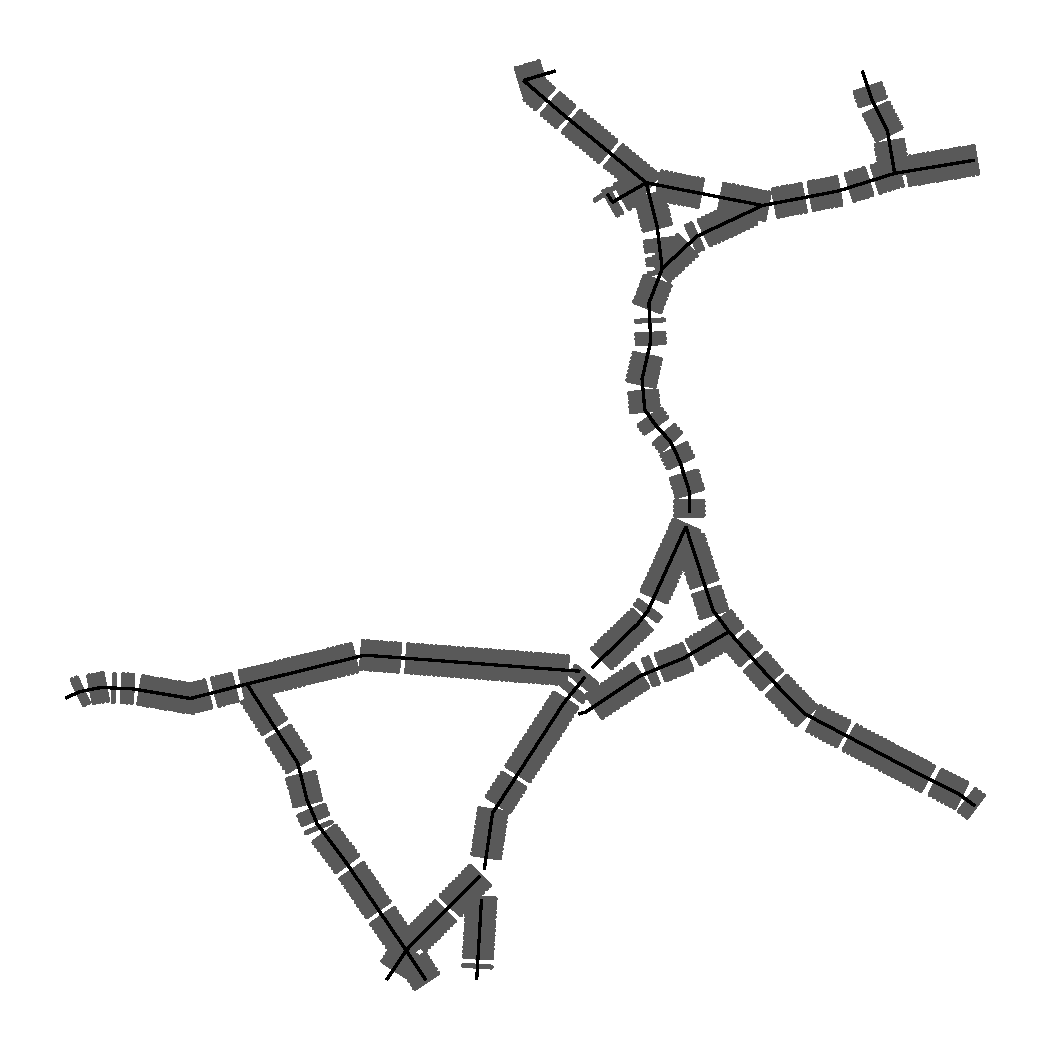
\includegraphics[width=.75\linewidth]{figure/sample_fig-1} 

}

\caption[Sample lines extracted based on known road locations]{Sample lines extracted based on known road locations}\label{fig:sample_fig}
\end{figure}


\end{knitrout}

\chapter{Scripts}\label{c:script}

\section{Clean Data}
\begin{knitrout}\footnotesize
\definecolor{shadecolor}{rgb}{0.969, 0.969, 0.969}\color{fgcolor}\begin{kframe}
\begin{alltt}
\hlcom{# Source Scripts}
\hlkwd{source}\hlstd{(}\hlstr{"./functions.r"}\hlstd{)}

\hlcom{# Create las catalog with all .laz files}
\hlstd{ctg} \hlkwb{<-} \hlkwd{catalog}\hlstd{(}\hlstr{"../data/point/"}\hlstd{)}
\hlkwd{opt_chunk_size}\hlstd{(ctg)} \hlkwb{<-} \hlnum{500}
\hlkwd{opt_chunk_buffer}\hlstd{(ctg)} \hlkwb{<-} \hlnum{20}

\hlcom{# create lax file to index + speed up process}
\hlkwd{plan}\hlstd{(multisession,} \hlkwc{workers} \hlstd{=} \hlnum{6L}\hlstd{)}
\hlkwd{set_lidr_threads}\hlstd{(}\hlnum{12L}\hlstd{)}
\hlcom{# speed up lax computation time}
\hlstd{lidR}\hlopt{:::}\hlkwd{catalog_laxindex}\hlstd{(ctg)}

\hlcom{# ctg to points csv}
\hlstd{las} \hlkwb{<-} \hlkwd{catalog_apply}\hlstd{(ctg, ctg_to_df)}
\hlstd{las} \hlkwb{<-} \hlkwd{do.call}\hlstd{(rbind, las)}
\hlstd{las} \hlkwb{<-} \hlstd{las} \hlopt
    \hlkwd{select}\hlstd{(}\hlopt{-}\hlkwd{c}\hlstd{(}
        \hlstd{Synthetic_flag,}
        \hlstd{Keypoint_flag,}
        \hlstd{Withheld_flag}
    \hlstd{))}

\hlkwd{fwrite}\hlstd{(las,} \hlstr{"../data/point/points.csv"}\hlstd{)}

\hlcom{# filter using sql expressions why not}
\hlcom{# very very slow to read in full gpkg, don't run unless new data added}
\hlcom{# roads <- st_read("../data/osroads/oproad_gpkg_gb/data/oproad_gb.gpkg",}
\hlcom{#    layer = "RoadLink", query =}
\hlcom{#        "SELECT * FROM RoadLink WHERE}
\hlcom{#         formOfWay = \textbackslash{}"Single Carriageway\textbackslash{}" AND}
\hlcom{#         roadFunction <> \textbackslash{}"Restricted Local Access Road\textbackslash{}" "}
\hlcom{# ) %>%}
\hlcom{#    st_zm() # remove z axis}
\hlcom{#}
\hlcom{# roads <- as_Spatial(roads)}
\hlcom{# roads <- raster::crop(roads, as.matrix(extent(ctg))) %>%}
\hlcom{#    st_as_sf()}

\hlcom{# st_write(roads, "../data/osroads/oproad_crop.gpkg")}

\hlstd{roads} \hlkwb{<-} \hlkwd{st_read}\hlstd{(}\hlstr{"../data/osroads/oproad_crop.gpkg"}\hlstd{)} \hlopt
    \hlkwd{mutate}\hlstd{(}
        \hlkwc{len} \hlstd{=} \hlkwd{as.numeric}\hlstd{(}\hlkwd{st_length}\hlstd{(geom)),}
        \hlkwc{road_id} \hlstd{=} \hlkwd{paste0}\hlstd{(}\hlstr{"road_"}\hlstd{,} \hlkwd{row_number}\hlstd{())}
    \hlstd{)} \hlopt
    \hlkwd{select}\hlstd{(}\hlkwd{c}\hlstd{(road_id, roadFunction, len, geom))} \hlopt
    \hlkwd{subset}\hlstd{(len} \hlopt{>} \hlnum{50}\hlstd{)}

\hlcom{# keep line polys}
\hlstd{roads_line} \hlkwb{<-} \hlstd{roads}

\hlcom{# one buffer to include non road points, 1m buffer to show only road points}
\hlstd{roads_buff} \hlkwb{<-} \hlkwd{st_buffer}\hlstd{(roads,} \hlnum{30}\hlstd{)}
\hlstd{roads} \hlkwb{<-} \hlkwd{st_buffer}\hlstd{(roads,} \hlnum{1}\hlstd{)}
\hlstd{roads_buff_union} \hlkwb{<-} \hlkwd{st_union}\hlstd{(roads_buff)}

\hlcom{# write all outputs to files}
\hlkwd{st_write}\hlstd{(roads,} \hlstr{"../data/derived/roads/roads.gpkg"}\hlstd{,}
    \hlkwc{delete_layer} \hlstd{=} \hlnum{TRUE}
\hlstd{)}
\hlkwd{st_write}\hlstd{(roads_line,} \hlstr{"../data/derived/roads/roads_line.gpkg"}\hlstd{,}
    \hlkwc{delete_layer} \hlstd{=} \hlnum{TRUE}
\hlstd{)}
\hlkwd{st_write}\hlstd{(roads_buff,} \hlstr{"../data/derived/roads/roads_buff.gpkg"}\hlstd{,}
    \hlkwc{delete_layer} \hlstd{=} \hlnum{TRUE}
\hlstd{)}

\hlkwd{st_write}\hlstd{(roads_buff_union,} \hlstr{"../data/derived/roads/roads_buff_diss.gpkg"}\hlstd{,}
    \hlkwc{delete_layer} \hlstd{=} \hlnum{TRUE}
\hlstd{)}

\hlstd{roads_buff} \hlkwb{<-} \hlkwd{st_read}\hlstd{(}\hlstr{"../data/derived/roads/roads_buff.gpkg"}\hlstd{)} \hlopt
    \hlkwd{as_Spatial}\hlstd{()}

\hlstd{ctg} \hlkwb{<-} \hlkwd{catalog}\hlstd{(}\hlstr{"../data/point/"}\hlstd{)}
\hlkwd{opt_output_files}\hlstd{(ctg)} \hlkwb{<-} \hlstr{"../data/derived/ctg_clean/\{ID\}_clean"}
\hlkwd{opt_chunk_size}\hlstd{(ctg)} \hlkwb{<-} \hlnum{500}
\hlkwd{opt_chunk_buffer}\hlstd{(ctg)} \hlkwb{<-} \hlnum{20}
\hlkwd{catalog_apply}\hlstd{(ctg, lidr_clean)}

\hlstd{ctg} \hlkwb{<-} \hlkwd{catalog}\hlstd{(}\hlstr{"../data/derived/ctg_clean/"}\hlstd{)}
\hlkwd{opt_output_files}\hlstd{(ctg)} \hlkwb{<-} \hlstr{"../data/derived/ctg_buff/\{ID\}_tile"}
\hlkwd{opt_chunk_size}\hlstd{(ctg)} \hlkwb{<-} \hlnum{500}
\hlkwd{opt_chunk_buffer}\hlstd{(ctg)} \hlkwb{<-} \hlnum{20}
\hlkwd{catalog_apply}\hlstd{(ctg, extract_buff, roads_buff)}

\hlstd{ctg} \hlkwb{<-} \hlkwd{catalog}\hlstd{(}\hlstr{"../data/derived/ctg_buff/"}\hlstd{)}
\hlkwd{opt_output_files}\hlstd{(ctg)} \hlkwb{<-} \hlstr{"../data/derived/ctg/\{ID\}_tile"}
\hlkwd{opt_chunk_size}\hlstd{(ctg)} \hlkwb{<-} \hlnum{500}
\hlkwd{opt_chunk_buffer}\hlstd{(ctg)} \hlkwb{<-} \hlnum{20}
\hlkwd{catalog_apply}\hlstd{(ctg, las_filter_noise,} \hlkwc{sensitivity} \hlstd{=} \hlnum{1.2}\hlstd{)}

\hlcom{# non normalised ctg}
\hlstd{ctg_notnorm} \hlkwb{<-} \hlkwd{catalog}\hlstd{(}\hlstr{"../data/point/"}\hlstd{)}
\hlkwd{opt_output_files}\hlstd{(ctg_notnorm)} \hlkwb{<-} \hlstr{"../data/derived/ctg_notnorm/\{ID\}_tile"}
\hlkwd{opt_chunk_size}\hlstd{(ctg_notnorm)} \hlkwb{<-} \hlnum{500}
\hlkwd{opt_chunk_buffer}\hlstd{(ctg_notnorm)} \hlkwb{<-} \hlnum{20}
\hlkwd{catalog_apply}\hlstd{(ctg_notnorm, extract_buff, roads_buff)}

\hlcom{# read in written roads file}
\hlstd{roads} \hlkwb{<-} \hlkwd{read_sf}\hlstd{(}\hlstr{"../data/derived/roads/roads.gpkg"}\hlstd{)}

\hlcom{# find roads extent shows study area + used for aerial imagery from digimaps}
\hlstd{extent} \hlkwb{<-} \hlkwd{st_as_sfc}\hlstd{(}\hlkwd{st_bbox}\hlstd{(roads))}

\hlcom{# Write extent shapefile}
\hlkwd{st_write}\hlstd{(extent,} \hlstr{"../data/derived/extent/extent.gpkg"}\hlstd{,} \hlkwc{delete_layer} \hlstd{=} \hlnum{TRUE}\hlstd{)}
\end{alltt}
\end{kframe}
\end{knitrout}


\section{Create Sample lines}
\begin{knitrout}\footnotesize
\definecolor{shadecolor}{rgb}{0.969, 0.969, 0.969}\color{fgcolor}\begin{kframe}
\begin{alltt}
\hlkwd{source}\hlstd{(}\hlstr{"./functions.r"}\hlstd{)}

\hlstd{centrelines} \hlkwb{<-} \hlkwd{read_sf}\hlstd{(}\hlstr{"../data/derived/roads/roads_line.gpkg"}\hlstd{)} \hlopt
    \hlkwd{st_set_crs}\hlstd{(}\hlnum{27700}\hlstd{)}

\hlstd{roads_split} \hlkwb{<-} \hlstd{centrelines} \hlopt \hlkwd{st_cast}\hlstd{(}\hlstr{"POINT"}\hlstd{)}

\hlstd{roads_split} \hlkwb{<-} \hlkwd{split}\hlstd{(roads_split,} \hlkwc{f} \hlstd{= roads_split}\hlopt{$}\hlstd{road_id)}

\hlstd{sample_lines} \hlkwb{<-} \hlkwd{lapply}\hlstd{(roads_split, compute_samples)}
\hlstd{sample_lines} \hlkwb{<-} \hlkwd{do.call}\hlstd{(rbind, sample_lines)}

\hlstd{sample_lines} \hlkwb{<-} \hlstd{sample_lines} \hlopt
    \hlkwd{st_set_crs}\hlstd{(}\hlnum{27700}\hlstd{)}
\hlcom{# label each sample}
\hlstd{sample_lines}\hlopt{$}\hlstd{sample_id} \hlkwb{<-} \hlkwd{seq.int}\hlstd{(}\hlkwd{nrow}\hlstd{(sample_lines))}

\hlkwd{write_sf}\hlstd{(sample_lines,} \hlstr{"../data/derived/roads/sample_lines.gpkg"}\hlstd{)}

\hlstd{ctg} \hlkwb{<-} \hlkwd{catalog}\hlstd{(}\hlstr{"../data/derived/ctg_buff/"}\hlstd{)}

\hlkwd{opt_chunk_size}\hlstd{(ctg)} \hlkwb{<-} \hlnum{500}
\hlkwd{plan}\hlstd{(multisession,} \hlkwc{workers} \hlstd{=} \hlnum{6L}\hlstd{)}
\hlkwd{set_lidr_threads}\hlstd{(}\hlnum{12L}\hlstd{)}

\hlcom{# remove points outside samples}
\hlstd{comb} \hlkwb{<-} \hlkwd{catalog_apply}\hlstd{(ctg, clip_samples, sample_lines)}
\hlstd{comb} \hlkwb{<-} \hlstd{comb} \hlkwb{<-} \hlkwd{do.call}\hlstd{(rbind, comb)}

\hlstd{roads} \hlkwb{<-} \hlkwd{st_read}\hlstd{(}\hlstr{"../data/derived/roads/roads.gpkg"}\hlstd{)} \hlopt
    \hlkwd{st_transform}\hlstd{(}\hlnum{27700}\hlstd{)}
\hlstd{roads_df} \hlkwb{<-} \hlstd{roads} \hlopt \hlkwd{st_drop_geometry}\hlstd{()}

\hlstd{comb} \hlkwb{<-} \hlstd{comb} \hlopt
    \hlkwd{st_transform}\hlstd{(}\hlnum{27700}\hlstd{)}

\hlstd{joined_output} \hlkwb{<-} \hlkwd{merge}\hlstd{(comb, roads_df,} \hlkwc{by} \hlstd{=} \hlstr{"road_id"}\hlstd{)}

\hlstd{int} \hlkwb{<-} \hlkwd{st_contains}\hlstd{(roads, joined_output,} \hlkwc{sparse} \hlstd{=} \hlnum{FALSE}\hlstd{)} \hlopt
    \hlkwd{colSums}\hlstd{()}

\hlstd{joined_output}\hlopt{$}\hlstd{road} \hlkwb{<-} \hlstd{int}

\hlcom{# turn to binary, some road buffers overlap}
\hlstd{joined_output}\hlopt{$}\hlstd{road} \hlkwb{<-} \hlkwd{as.numeric}\hlstd{(joined_output}\hlopt{$}\hlstd{road} \hlopt{>} \hlnum{0}\hlstd{)}

\hlcom{# aerial data}
\hlstd{jpgs} \hlkwb{<-} \hlkwd{Sys.glob}\hlstd{(}\hlstr{"../data/aerial/*.jpg"}\hlstd{)}
\hlstd{jpgs} \hlkwb{<-} \hlkwd{lapply}\hlstd{(jpgs, brick)}
\hlstd{grey_rasters} \hlkwb{<-} \hlkwd{lapply}\hlstd{(jpgs, greyscale)}
\hlstd{grey_rasters} \hlkwb{<-} \hlkwd{lapply}\hlstd{(grey_rasters, brick)}
\hlstd{aerial} \hlkwb{<-} \hlkwd{do.call}\hlstd{(merge, grey_rasters)}
\hlstd{aerial} \hlkwb{<-} \hlkwd{crop}\hlstd{(aerial, roads)}

\hlkwd{writeRaster}\hlstd{(aerial,} \hlstr{"../data/derived/aerial/aerial_crop.tif"}\hlstd{,}
    \hlkwc{format} \hlstd{=} \hlstr{"GTiff"}\hlstd{,} \hlkwc{overwrite} \hlstd{=} \hlnum{TRUE}
\hlstd{)}

\hlcom{# crop aerial data}
\hlstd{lum} \hlkwb{<-} \hlstd{raster}\hlopt{::}\hlkwd{extract}\hlstd{(aerial, joined_output)}
\hlstd{joined_output}\hlopt{$}\hlstd{lum} \hlkwb{<-} \hlkwd{as.numeric}\hlstd{(lum)}


\hlcom{# find dists from centrelines}
\hlstd{joined_output} \hlkwb{<-} \hlkwd{split}\hlstd{(joined_output,} \hlkwc{f} \hlstd{= joined_output}\hlopt{$}\hlstd{road_id)}
\hlstd{centrelines} \hlkwb{<-} \hlkwd{split}\hlstd{(centrelines, centrelines}\hlopt{$}\hlstd{road_id)}

\hlstd{centrelines} \hlkwb{<-} \hlstd{centrelines[}\hlkwd{names}\hlstd{(joined_output)]}

\hlstd{dists} \hlkwb{<-} \hlkwd{mapply}\hlstd{(}
    \hlstd{find_dists,}
    \hlstd{joined_output,}
    \hlstd{centrelines}
\hlstd{)}

\hlstd{joined_output} \hlkwb{<-} \hlkwd{do.call}\hlstd{(rbind, joined_output)}
\hlstd{dists} \hlkwb{<-} \hlkwd{do.call}\hlstd{(rbind, dists)}
\hlstd{joined_output}\hlopt{$}\hlstd{dists} \hlkwb{<-} \hlstd{dists}

\hlstd{coords} \hlkwb{<-} \hlstd{joined_output} \hlopt
    \hlkwd{st_coordinates}\hlstd{()}

\hlcom{# change to data.frame}
\hlstd{joined_output} \hlkwb{<-} \hlstd{joined_output} \hlopt
    \hlkwd{st_drop_geometry}\hlstd{()} \hlopt
    \hlkwd{mutate}\hlstd{(}
        \hlkwc{X} \hlstd{= coords[,} \hlnum{1}\hlstd{],}
        \hlkwc{Y} \hlstd{= coords[,} \hlnum{2}\hlstd{]}
    \hlstd{)}

\hlkwd{fwrite}\hlstd{(joined_output,} \hlstr{"../data/derived/model_data/sampled_las.csv"}\hlstd{)}
\end{alltt}
\end{kframe}
\end{knitrout}

\section{Linear Models and Improved Centrelines}
\begin{knitrout}\footnotesize
\definecolor{shadecolor}{rgb}{0.969, 0.969, 0.969}\color{fgcolor}\begin{kframe}
\begin{alltt}
\hlkwd{source}\hlstd{(}\hlstr{"./functions.r"}\hlstd{)}
\hlstd{sampled_las} \hlkwb{<-} \hlkwd{fread}\hlstd{(}\hlstr{"../data/derived/model_data/sampled_las.csv"}\hlstd{)}

\hlcom{# ground pts only}
\hlstd{sampled_las} \hlkwb{<-} \hlstd{sampled_las[sampled_las}\hlopt{$}\hlstd{Classification} \hlopt{==} \hlnum{2}\hlstd{, ]}

\hlcom{# global linear model: unfiltered}
\hlcom{# for this section see social survey + ss assessment 2}
\hlstd{f1} \hlkwb{<-} \hlkwd{as.formula}\hlstd{(}\hlstr{"road ~ Intensity + lum + dists + Z + NumberOfReturns"}\hlstd{)}
\hlstd{lm1} \hlkwb{<-} \hlkwd{lm}\hlstd{(}\hlkwc{data} \hlstd{= sampled_las,} \hlkwc{formula} \hlstd{= f1)}
\hlstd{lm1_pred} \hlkwb{<-} \hlkwd{predict}\hlstd{(lm1, sampled_las,} \hlkwc{type} \hlstd{=} \hlstr{"response"}\hlstd{)}

\hlstd{sampled_las}\hlopt{$}\hlstd{lm1_pred} \hlkwb{<-} \hlstd{lm1_pred}
\hlstd{sampled_las}\hlopt{$}\hlstd{lm1_dum} \hlkwb{<-} \hlkwd{ifelse}\hlstd{(sampled_las}\hlopt{$}\hlstd{lm1_pred} \hlopt{>}
    \hlkwd{quantile}\hlstd{(sampled_las}\hlopt{$}\hlstd{lm1_pred,} \hlnum{.95}\hlstd{),} \hlnum{1}\hlstd{,} \hlnum{0}\hlstd{)}

\hlstd{sampled_las}\hlopt{$}\hlstd{lm1_pred} \hlkwb{<-} \hlstd{lm1_pred}
\hlstd{sampled_las}\hlopt{$}\hlstd{lm1_dum90} \hlkwb{<-} \hlkwd{ifelse}\hlstd{(sampled_las}\hlopt{$}\hlstd{lm1_pred} \hlopt{>}
    \hlkwd{quantile}\hlstd{(sampled_las}\hlopt{$}\hlstd{lm1_pred,} \hlnum{.90}\hlstd{),} \hlnum{1}\hlstd{,} \hlnum{0}\hlstd{)}

\hlstd{sampled_las}\hlopt{$}\hlstd{lm1_pred} \hlkwb{<-} \hlstd{lm1_pred}
\hlstd{sampled_las}\hlopt{$}\hlstd{lm1_dum80} \hlkwb{<-} \hlkwd{ifelse}\hlstd{(sampled_las}\hlopt{$}\hlstd{lm1_pred} \hlopt{>}
    \hlkwd{quantile}\hlstd{(sampled_las}\hlopt{$}\hlstd{lm1_pred,} \hlnum{.80}\hlstd{),} \hlnum{1}\hlstd{,} \hlnum{0}\hlstd{)}

\hlkwd{fwrite}\hlstd{(sampled_las,} \hlstr{"../data/derived/model_data/linearmodels.csv"}\hlstd{)}
\end{alltt}
\end{kframe}
\end{knitrout}

\section{Road Widths}
\begin{knitrout}\footnotesize
\definecolor{shadecolor}{rgb}{0.969, 0.969, 0.969}\color{fgcolor}\begin{kframe}
\begin{alltt}
\hlkwd{source}\hlstd{(}\hlstr{"./functions.r"}\hlstd{)}
\hlcom{## ---- widths}
\hlstd{road_lm} \hlkwb{<-} \hlkwd{fread}\hlstd{(}\hlstr{"../data/derived/model_data/linearmodels.csv"}\hlstd{)} \hlopt
    \hlkwd{as.data.frame}\hlstd{()} \hlopt
    \hlkwd{st_as_sf}\hlstd{(}\hlkwc{coords} \hlstd{=} \hlkwd{c}\hlstd{(}\hlstr{"X"}\hlstd{,} \hlstr{"Y"}\hlstd{),} \hlkwc{crs} \hlstd{=} \hlnum{27700}\hlstd{)}

\hlstd{roads} \hlkwb{<-} \hlkwd{st_read}\hlstd{(}\hlstr{"../data/derived/roads/roads_line.gpkg"}\hlstd{)}
\hlstd{roads_5m} \hlkwb{<-} \hlkwd{st_read}\hlstd{(}\hlstr{"../data/derived/roads/roads_line.gpkg"}\hlstd{)} \hlopt
    \hlkwd{st_buffer}\hlstd{(}\hlnum{5}\hlstd{)}

\hlstd{road_lm90} \hlkwb{<-} \hlstd{road_lm[road_lm}\hlopt{$}\hlstd{lm1_dum90} \hlopt{==} \hlnum{1}\hlstd{, ]}
\hlcom{# find improved centrelines}
\hlstd{fixed_cents} \hlkwb{<-} \hlkwd{list}\hlstd{(}
    \hlstd{road_lm90}
\hlstd{)}

\hlcom{# includes all filtering, max dist points}
\hlstd{fixed_cents} \hlkwb{<-} \hlkwd{lapply}\hlstd{(fixed_cents, max_lines,} \hlkwc{cents} \hlstd{= roads)}

\hlstd{fixed_cents} \hlkwb{<-} \hlkwd{do.call}\hlstd{(rbind, fixed_cents)}
\hlstd{fixed_cents} \hlkwb{<-} \hlstd{fixed_cents} \hlopt
    \hlkwd{mutate}\hlstd{(}\hlkwc{rowid} \hlstd{=} \hlkwd{row_number}\hlstd{())}

\hlstd{mid_point} \hlkwb{<-} \hlkwd{split}\hlstd{(fixed_cents, fixed_cents}\hlopt{$}\hlstd{rowid)}
\hlstd{mid_points} \hlkwb{<-} \hlkwd{lapply}\hlstd{(mid_point, mid_pts)}

\hlstd{mid_points} \hlkwb{<-} \hlkwd{do.call}\hlstd{(rbind, mid_points)}
\hlstd{mid_points} \hlkwb{<-} \hlstd{mid_points} \hlopt
    \hlkwd{st_join}\hlstd{(roads_5m)}
\hlstd{mid_rds} \hlkwb{<-} \hlkwd{split}\hlstd{(mid_points, mid_points}\hlopt{$}\hlstd{road_id)}

\hlcom{# remove empty geoms}
\hlstd{mid_rds} \hlkwb{<-} \hlkwd{Filter}\hlstd{(}\hlkwa{function}\hlstd{(}\hlkwc{x}\hlstd{)} \hlkwd{dim}\hlstd{(x)[}\hlnum{1}\hlstd{]} \hlopt{>} \hlnum{0}\hlstd{, mid_rds)}
\hlstd{cents} \hlkwb{<-} \hlkwd{lapply}\hlstd{(mid_rds, true_cents)}
\hlstd{cents} \hlkwb{<-} \hlkwd{compact}\hlstd{(cents)}
\hlstd{cents} \hlkwb{<-} \hlkwd{do.call}\hlstd{(rbind, cents)}

\hlkwd{st_write}\hlstd{(cents,} \hlstr{"../data/derived/roads/cent_iteration1.gpkg"}\hlstd{,}
    \hlkwc{layer_options} \hlstd{=} \hlstr{"OVERWRITE=yes"}
\hlstd{)}

\hlcom{## ---- angles}
\hlstd{roads_split} \hlkwb{<-} \hlkwd{st_read}\hlstd{(}\hlstr{"../data/derived/roads/roads_line.gpkg"}\hlstd{)} \hlopt
    \hlkwd{st_cast}\hlstd{(}\hlstr{"POINT"}\hlstd{)} \hlopt
    \hlkwd{st_set_crs}\hlstd{(}\hlnum{27700}\hlstd{)}

\hlstd{roads_split} \hlkwb{<-} \hlkwd{split}\hlstd{(roads_split, roads_split}\hlopt{$}\hlstd{road_id)}

\hlstd{angles} \hlkwb{<-} \hlkwd{lapply}\hlstd{(roads_split, road_angles)}
\hlstd{angles} \hlkwb{<-} \hlkwd{do.call}\hlstd{(rbind, angles)}
\hlkwd{row.names}\hlstd{(angles)} \hlkwb{<-} \hlkwa{NULL}
\hlstd{angles} \hlkwb{<-} \hlstd{angles} \hlopt
    \hlkwd{as.data.frame}\hlstd{()}
\hlkwd{names}\hlstd{(angles)} \hlkwb{<-} \hlkwd{c}\hlstd{(}\hlstr{"angle"}\hlstd{,} \hlstr{"road_id"}\hlstd{)}
\hlstd{angles}\hlopt{$}\hlstd{angle} \hlkwb{<-} \hlkwd{as.numeric}\hlstd{(}\hlkwd{unfactor}\hlstd{(angles}\hlopt{$}\hlstd{angle))}

\hlstd{angles} \hlkwb{<-} \hlstd{angles} \hlopt
    \hlkwd{group_by}\hlstd{(road_id)} \hlopt
    \hlkwd{summarise}\hlstd{(}
        \hlkwc{mean_angle} \hlstd{=} \hlkwd{mean}\hlstd{(angle),}
        \hlkwc{max_angle} \hlstd{=} \hlkwd{max}\hlstd{(angle)}
    \hlstd{)}

\hlstd{roads} \hlkwb{<-} \hlkwd{merge}\hlstd{(roads, angles,} \hlkwc{by} \hlstd{=} \hlstr{"road_id"}\hlstd{)}

\hlcom{## ---- heights}
\hlcom{# Non-normalised las files}
\hlstd{sample_lines} \hlkwb{<-} \hlkwd{st_read}\hlstd{(}\hlstr{"../data/derived/roads/sample_lines.gpkg"}\hlstd{)} \hlopt
    \hlkwd{st_set_crs}\hlstd{(}\hlnum{27700}\hlstd{)}
\hlstd{roads_1m} \hlkwb{<-} \hlkwd{st_read}\hlstd{(}\hlstr{"../data/derived/roads/roads.gpkg"}\hlstd{)}
\hlstd{ctg} \hlkwb{<-} \hlkwd{catalog}\hlstd{(}\hlstr{"../data/derived/ctg_notnorm/"}\hlstd{)}
\hlkwd{opt_chunk_size}\hlstd{(ctg)} \hlkwb{<-} \hlnum{500}
\hlkwd{plan}\hlstd{(multisession,} \hlkwc{workers} \hlstd{=} \hlnum{6L}\hlstd{)}
\hlkwd{set_lidr_threads}\hlstd{(}\hlnum{12L}\hlstd{)}

\hlcom{# remove points outside samples}
\hlstd{las_rds} \hlkwb{<-} \hlkwd{catalog_apply}\hlstd{(ctg, clip_samples, sample_lines)}
\hlstd{las_rds} \hlkwb{<-} \hlkwd{do.call}\hlstd{(rbind, las_rds)}

\hlstd{las_rds} \hlkwb{<-} \hlstd{las_rds[las_rds}\hlopt{$}\hlstd{NumberOfReturns} \hlopt{==} \hlnum{1} \hlopt{&}
    \hlstd{las_rds}\hlopt{$}\hlstd{Classification} \hlopt{==} \hlnum{2}\hlstd{, ]}

\hlstd{rds} \hlkwb{<-} \hlkwd{st_read}\hlstd{(}\hlstr{"../data/derived/roads/roads.gpkg"}\hlstd{)} \hlopt
    \hlkwd{st_transform}\hlstd{(}\hlnum{27700}\hlstd{)}

\hlstd{rd_line} \hlkwb{<-} \hlkwd{st_read}\hlstd{(}\hlstr{"../data/derived/roads/roads_line.gpkg"}\hlstd{,} \hlkwc{quiet} \hlstd{=} \hlnum{TRUE}\hlstd{)} \hlopt
    \hlkwd{mutate}\hlstd{(}\hlkwc{len} \hlstd{=} \hlkwd{as.numeric}\hlstd{(}\hlkwd{st_length}\hlstd{(geom)))} \hlopt
    \hlkwd{select}\hlstd{(}\hlkwd{c}\hlstd{(road_id, len))} \hlopt
    \hlkwd{st_drop_geometry}\hlstd{()}

\hlstd{roads_df} \hlkwb{<-} \hlstd{rds} \hlopt \hlkwd{st_drop_geometry}\hlstd{()}

\hlstd{las_rds} \hlkwb{<-} \hlstd{las_rds} \hlopt
    \hlkwd{st_transform}\hlstd{(}\hlnum{27700}\hlstd{)}

\hlstd{las_rds} \hlkwb{<-} \hlkwd{merge}\hlstd{(las_rds, roads_df,} \hlkwc{by} \hlstd{=} \hlstr{"road_id"}\hlstd{)}

\hlstd{int} \hlkwb{<-} \hlkwd{st_contains}\hlstd{(roads_1m, las_rds,} \hlkwc{sparse} \hlstd{=} \hlnum{FALSE}\hlstd{)} \hlopt
    \hlkwd{colSums}\hlstd{()}

\hlstd{las_rds}\hlopt{$}\hlstd{road} \hlkwb{<-} \hlstd{int}

\hlcom{# remove overlapping road points}
\hlstd{las_rds} \hlkwb{<-} \hlstd{las_rds[las_rds}\hlopt{$}\hlstd{road} \hlopt{<} \hlnum{2}\hlstd{, ]}
\hlcom{# turn to binary (might not be needed)}
\hlstd{las_rds}\hlopt{$}\hlstd{road} \hlkwb{<-} \hlkwd{as.numeric}\hlstd{(las_rds}\hlopt{$}\hlstd{road} \hlopt{>} \hlnum{0}\hlstd{)}

\hlstd{las_rds} \hlkwb{<-} \hlstd{las_rds[las_rds}\hlopt{$}\hlstd{road} \hlopt{==} \hlnum{1}\hlstd{, ]}

\hlstd{las_rds} \hlkwb{<-} \hlkwd{split}\hlstd{(las_rds, las_rds}\hlopt{$}\hlstd{sample_id)}

\hlstd{las_rds} \hlkwb{<-} \hlkwd{lapply}\hlstd{(las_rds, filter_returns)}

\hlstd{las_rds} \hlkwb{<-} \hlstd{las_rds} \hlopt
    \hlkwd{compact}\hlstd{()}

\hlstd{las_rds} \hlkwb{<-} \hlkwd{do.call}\hlstd{(rbind, las_rds)}

\hlstd{las_height} \hlkwb{<-} \hlkwd{split}\hlstd{(las_rds, las_rds}\hlopt{$}\hlstd{road_id)}

\hlstd{las_height} \hlkwb{<-} \hlkwd{lapply}\hlstd{(las_height, height_change)}

\hlstd{las_height} \hlkwb{<-} \hlkwd{do.call}\hlstd{(rbind, las_height)}
\hlstd{las_height} \hlkwb{<-} \hlkwd{as.data.frame}\hlstd{(las_height)}

\hlkwd{names}\hlstd{(las_height)} \hlkwb{<-} \hlkwd{c}\hlstd{(}\hlstr{"road_id"}\hlstd{,} \hlstr{"Z"}\hlstd{)}
\hlstd{las_height} \hlkwb{<-} \hlstd{las_height} \hlopt
    \hlkwd{merge}\hlstd{(rd_line,} \hlkwc{by} \hlstd{=} \hlstr{"road_id"}\hlstd{)}

\hlstd{las_height} \hlkwb{<-} \hlstd{las_height} \hlopt
    \hlkwd{group_by}\hlstd{(road_id)} \hlopt
    \hlkwd{summarise}\hlstd{(}
        \hlkwc{tot_z} \hlstd{=} \hlkwd{sum}\hlstd{(}\hlkwd{as.numeric}\hlstd{(}\hlkwd{unfactor}\hlstd{(Z)))} \hlopt{/} \hlstd{(}\hlkwd{mean}\hlstd{(len)} \hlopt{/} \hlnum{1000}\hlstd{),}
    \hlstd{)} \hlopt
    \hlkwd{drop_na}\hlstd{()}

\hlstd{roads} \hlkwb{<-} \hlkwd{merge}\hlstd{(roads, las_height,} \hlkwc{by} \hlstd{=} \hlstr{"road_id"}\hlstd{)}

\hlcom{## ---- surface_qual}
\hlstd{las_qual} \hlkwb{<-} \hlstd{las_rds} \hlopt
    \hlkwd{group_by}\hlstd{(road_id)} \hlopt
    \hlkwd{summarise}\hlstd{(}
        \hlkwc{mean_int} \hlstd{=} \hlkwd{mean}\hlstd{(Intensity),}
        \hlkwc{range_int} \hlstd{=} \hlkwd{max}\hlstd{(Intensity)} \hlopt{-} \hlkwd{min}\hlstd{(Intensity)}
    \hlstd{)} \hlopt
    \hlkwd{drop_na}\hlstd{()} \hlopt
    \hlkwd{select}\hlstd{(}\hlkwd{c}\hlstd{(road_id, mean_int, range_int))}

\hlstd{roads} \hlkwb{<-} \hlkwd{merge}\hlstd{(roads, las_qual,} \hlkwc{by} \hlstd{=} \hlstr{"road_id"}\hlstd{)} \hlopt
    \hlkwd{st_drop_geometry}\hlstd{()}

\hlcom{## ---- asdf}
\hlkwd{write.csv}\hlstd{(roads,} \hlstr{"../data/final_data/final.csv"}\hlstd{)}
\end{alltt}
\end{kframe}
\end{knitrout}

\section{Improved Centreline Models}
\begin{knitrout}\footnotesize
\definecolor{shadecolor}{rgb}{0.969, 0.969, 0.969}\color{fgcolor}\begin{kframe}
\begin{alltt}
\hlkwd{source}\hlstd{(}\hlstr{"./functions.r"}\hlstd{)}
\hlstd{cent1} \hlkwb{<-} \hlkwd{st_read}\hlstd{(}\hlstr{"../data/derived/roads/cent_iteration1.gpkg"}\hlstd{)} \hlopt
    \hlkwd{st_transform}\hlstd{(}\hlnum{27700}\hlstd{)}
\hlstd{sampled_las} \hlkwb{<-} \hlkwd{fread}\hlstd{(}\hlstr{"../data/derived/model_data/sampled_las.csv"}\hlstd{)} \hlopt
    \hlkwd{as.data.frame}\hlstd{()} \hlopt
    \hlkwd{st_as_sf}\hlstd{(}\hlkwc{coords} \hlstd{=} \hlkwd{c}\hlstd{(}\hlstr{"X"}\hlstd{,} \hlstr{"Y"}\hlstd{),} \hlkwc{crs} \hlstd{=} \hlnum{27700}\hlstd{)}
\hlstd{aerial} \hlkwb{<-} \hlkwd{raster}\hlstd{(}\hlstr{"../data/derived/aerial/aerial_crop.tif"}\hlstd{)}


\hlcom{# improved roads centrelines}
\hlstd{roads} \hlkwb{<-} \hlstd{cent1} \hlopt
    \hlkwd{st_buffer}\hlstd{(}\hlnum{2}\hlstd{)}

\hlstd{roads_df} \hlkwb{<-} \hlstd{roads} \hlopt \hlkwd{st_drop_geometry}\hlstd{()}

\hlstd{joined_output} \hlkwb{<-} \hlkwd{merge}\hlstd{(sampled_las, roads_df,} \hlkwc{by} \hlstd{=} \hlstr{"road_id"}\hlstd{)}

\hlstd{int} \hlkwb{<-} \hlkwd{st_contains}\hlstd{(roads, joined_output,} \hlkwc{sparse} \hlstd{=} \hlnum{FALSE}\hlstd{)} \hlopt
    \hlkwd{colSums}\hlstd{()}

\hlstd{joined_output}\hlopt{$}\hlstd{road} \hlkwb{<-} \hlstd{int}

\hlcom{# turn to binary, some road buffers overlap}
\hlstd{joined_output}\hlopt{$}\hlstd{road} \hlkwb{<-} \hlkwd{as.numeric}\hlstd{(joined_output}\hlopt{$}\hlstd{road} \hlopt{>} \hlnum{0}\hlstd{)}

\hlcom{# crop aerial data}
\hlstd{lum} \hlkwb{<-} \hlstd{raster}\hlopt{::}\hlkwd{extract}\hlstd{(aerial, joined_output)}
\hlstd{joined_output}\hlopt{$}\hlstd{lum} \hlkwb{<-} \hlkwd{as.numeric}\hlstd{(lum)}

\hlcom{# find dists from centrelines}
\hlstd{joined_output} \hlkwb{<-} \hlkwd{split}\hlstd{(joined_output,} \hlkwc{f} \hlstd{= joined_output}\hlopt{$}\hlstd{road_id)}
\hlstd{centrelines} \hlkwb{<-} \hlkwd{split}\hlstd{(cent1, cent1}\hlopt{$}\hlstd{road_id)}

\hlstd{centrelines} \hlkwb{<-} \hlstd{centrelines[}\hlkwd{names}\hlstd{(joined_output)]}

\hlstd{dists} \hlkwb{<-} \hlkwd{mapply}\hlstd{(}
    \hlstd{find_dists,}
    \hlstd{joined_output,}
    \hlstd{centrelines}
\hlstd{)}

\hlstd{joined_output} \hlkwb{<-} \hlkwd{do.call}\hlstd{(rbind, joined_output)}
\hlstd{dists} \hlkwb{<-} \hlkwd{do.call}\hlstd{(rbind, dists)}
\hlstd{joined_output}\hlopt{$}\hlstd{dists} \hlkwb{<-} \hlstd{dists}

\hlstd{coords} \hlkwb{<-} \hlstd{joined_output} \hlopt
    \hlkwd{st_coordinates}\hlstd{()}
\hlstd{cent1_las} \hlkwb{<-} \hlstd{joined_output} \hlopt
    \hlkwd{st_drop_geometry}\hlstd{()} \hlopt
    \hlkwd{mutate}\hlstd{(}
        \hlkwc{X} \hlstd{= coords[,} \hlnum{1}\hlstd{],}
        \hlkwc{Y} \hlstd{= coords[,} \hlnum{2}\hlstd{]}
    \hlstd{)}

\hlkwd{fwrite}\hlstd{(cent1_las,} \hlstr{"../data/derived/model_data/cent1_lm.csv"}\hlstd{)}

\hlcom{# linear models with improved centrelines}
\hlcom{# for this section see social survey + ss assessment 2}
\hlstd{f1} \hlkwb{<-} \hlkwd{as.formula}\hlstd{(}\hlstr{"road ~ Intensity + lum + dists + Z + NumberOfReturns"}\hlstd{)}
\hlstd{lm1} \hlkwb{<-} \hlkwd{lm}\hlstd{(}\hlkwc{data} \hlstd{= cent1_las,} \hlkwc{formula} \hlstd{= f1)}
\hlstd{lm1_pred} \hlkwb{<-} \hlkwd{predict}\hlstd{(lm1, cent1_las,} \hlkwc{type} \hlstd{=} \hlstr{"response"}\hlstd{)}

\hlstd{f2} \hlkwb{<-} \hlkwd{as.formula}\hlstd{(}\hlstr{"road ~ Intensity + dists + Z + NumberOfReturns"}\hlstd{)}
\hlstd{lm2} \hlkwb{<-} \hlkwd{lm}\hlstd{(}\hlkwc{data} \hlstd{= cent1_las,} \hlkwc{formula} \hlstd{= f2)}
\hlstd{lm2_pred} \hlkwb{<-} \hlkwd{predict}\hlstd{(lm2, cent1_las,} \hlkwc{type} \hlstd{=} \hlstr{"response"}\hlstd{)}

\hlstd{cent1_las}\hlopt{$}\hlstd{lm1_pred} \hlkwb{<-} \hlstd{lm1_pred}
\hlstd{cent1_las}\hlopt{$}\hlstd{lm1_dum} \hlkwb{<-} \hlkwd{ifelse}\hlstd{(cent1_las}\hlopt{$}\hlstd{lm1_pred} \hlopt{>}
    \hlkwd{quantile}\hlstd{(cent1_las}\hlopt{$}\hlstd{lm1_pred,} \hlnum{.95}\hlstd{),} \hlnum{1}\hlstd{,} \hlnum{0}\hlstd{)}

\hlstd{cent1_las}\hlopt{$}\hlstd{lm2_pred} \hlkwb{<-} \hlstd{lm2_pred}
\hlstd{cent1_las}\hlopt{$}\hlstd{lm2_dum} \hlkwb{<-} \hlkwd{ifelse}\hlstd{(cent1_las}\hlopt{$}\hlstd{lm2_pred} \hlopt{>}
    \hlkwd{quantile}\hlstd{(cent1_las}\hlopt{$}\hlstd{lm2_pred,} \hlnum{.95}\hlstd{),} \hlnum{1}\hlstd{,} \hlnum{0}\hlstd{)}


\hlcom{# individual linear probability model: has to filter out canopy: proof of concept}
\hlstd{cent1_las} \hlkwb{<-} \hlkwd{split}\hlstd{(cent1_las, cent1_las}\hlopt{$}\hlstd{sample_id)}
\hlstd{cent1_las} \hlkwb{<-} \hlkwd{lapply}\hlstd{(cent1_las, filter_returns)}
\hlstd{f1} \hlkwb{<-} \hlkwd{as.formula}\hlstd{(}\hlstr{"road ~ Intensity + dists + Z + NumberOfReturns"}\hlstd{)}
\hlstd{cent1_las} \hlkwb{<-} \hlkwd{lapply}\hlstd{(cent1_las, lm_compute,} \hlkwc{f} \hlstd{= f1)}
\hlstd{cent1_las} \hlkwb{<-} \hlkwd{do.call}\hlstd{(rbind, cent1_las)}

\hlkwd{fwrite}\hlstd{(cent1_las,} \hlstr{"../data/final_data/cent_lm.csv"}\hlstd{)}

\hlstd{lmi} \hlkwb{<-} \hlstd{cent1_las[cent1_las}\hlopt{$}\hlstd{I_dum} \hlopt{==} \hlnum{1}\hlstd{, ]} \hlopt
    \hlkwd{as.data.frame}\hlstd{()} \hlopt
    \hlkwd{st_as_sf}\hlstd{(}\hlkwc{coords} \hlstd{=} \hlkwd{c}\hlstd{(}\hlstr{"X"}\hlstd{,} \hlstr{"Y"}\hlstd{),} \hlkwc{crs} \hlstd{=} \hlnum{27700}\hlstd{)}
\hlstd{lm1} \hlkwb{<-} \hlstd{cent1_las[cent1_las}\hlopt{$}\hlstd{lm1_dum} \hlopt{==} \hlnum{1}\hlstd{, ]} \hlopt
    \hlkwd{as.data.frame}\hlstd{()} \hlopt
    \hlkwd{st_as_sf}\hlstd{(}\hlkwc{coords} \hlstd{=} \hlkwd{c}\hlstd{(}\hlstr{"X"}\hlstd{,} \hlstr{"Y"}\hlstd{),} \hlkwc{crs} \hlstd{=} \hlnum{27700}\hlstd{)}
\hlstd{lm2} \hlkwb{<-} \hlstd{cent1_las[cent1_las}\hlopt{$}\hlstd{lm2_dum} \hlopt{==} \hlnum{1}\hlstd{, ]} \hlopt
    \hlkwd{as.data.frame}\hlstd{()} \hlopt
    \hlkwd{st_as_sf}\hlstd{(}\hlkwc{coords} \hlstd{=} \hlkwd{c}\hlstd{(}\hlstr{"X"}\hlstd{,} \hlstr{"Y"}\hlstd{),} \hlkwc{crs} \hlstd{=} \hlnum{27700}\hlstd{)}

\hlstd{lm2} \hlkwb{<-} \hlkwd{split}\hlstd{(lm2, lm2}\hlopt{$}\hlstd{road_id)}
\hlstd{tot_pts} \hlkwb{<-} \hlkwd{lapply}\hlstd{(lm2,} \hlkwa{function}\hlstd{(}\hlkwc{x}\hlstd{) \{}
    \hlstd{tot_pts} \hlkwb{<-} \hlkwd{nrow}\hlstd{(x)}
    \hlkwd{return}\hlstd{(tot_pts)}
\hlstd{\})}
\hlstd{lm2} \hlkwb{<-} \hlkwd{do.call}\hlstd{(rbind, lm2)}

\hlstd{lm_max_widths} \hlkwb{<-} \hlkwd{list}\hlstd{(lmi, lm1, lm2)}

\hlstd{road_buff} \hlkwb{<-} \hlkwd{st_read}\hlstd{(}\hlstr{"../data/derived/roads/roads_buff.gpkg"}\hlstd{)}

\hlstd{centrelines} \hlkwb{<-} \hlkwd{do.call}\hlstd{(rbind, centrelines)}
\hlcom{# includes all filtering, max dist points}
\hlstd{lm_max_widths} \hlkwb{<-} \hlkwd{lapply}\hlstd{(lm_max_widths, max_lines,} \hlkwc{cents} \hlstd{= centrelines)}

\hlstd{lm_max_widths} \hlkwb{<-} \hlkwd{lapply}\hlstd{(lm_max_widths,} \hlkwa{function}\hlstd{(}\hlkwc{x}\hlstd{) \{}
    \hlstd{x} \hlkwb{<-} \hlstd{x[x}\hlopt{$}\hlstd{length} \hlopt{<} \hlnum{8} \hlopt{&} \hlstd{x}\hlopt{$}\hlstd{length} \hlopt{>} \hlnum{2}\hlstd{, ]}
    \hlstd{x} \hlkwb{<-} \hlstd{x[}\hlopt{!}\hlkwd{is.na}\hlstd{(x}\hlopt{$}\hlstd{road_id), ]}
\hlstd{\})}

\hlcom{# save lines for comparison}
\hlkwa{for} \hlstd{(i} \hlkwa{in} \hlnum{1}\hlopt{:}\hlkwd{length}\hlstd{(lm_max_widths)) \{}
    \hlkwd{st_write}\hlstd{(lm_max_widths[[i]],} \hlkwd{paste0}\hlstd{(}\hlstr{"../data/final_data/widths_"}\hlstd{, i,} \hlstr{".gpkg"}\hlstd{),}
        \hlkwc{layer_options} \hlstd{=} \hlstr{"OVERWRITE=YES"}
    \hlstd{)}
\hlstd{\}}

\hlcom{####}

\hlstd{centrelines} \hlkwb{<-} \hlkwd{st_read}\hlstd{(}\hlstr{"../data/derived/roads/cent_iteration1.gpkg"}\hlstd{)}
\hlstd{linear_widths} \hlkwb{<-} \hlkwd{lapply}\hlstd{(lm_max_widths, model_comparison)}
\hlstd{linear_widths} \hlkwb{<-} \hlstd{linear_widths} \hlopt
    \hlkwd{reduce}\hlstd{(left_join,} \hlkwc{by} \hlstd{=} \hlstr{"road_id"}\hlstd{)}

\hlkwd{names}\hlstd{(linear_widths)} \hlkwb{<-} \hlkwd{c}\hlstd{(}
    \hlstr{"road_id"}\hlstd{,}
    \hlstr{"lmi_mean"}\hlstd{,}
    \hlstr{"lm1_mean"}\hlstd{,}
    \hlstr{"lm2_mean"}
\hlstd{)}
\hlstd{tot_pts} \hlkwb{<-} \hlkwd{do.call}\hlstd{(rbind, tot_pts)} \hlopt
    \hlkwd{as.data.frame}\hlstd{()} \hlopt
    \hlkwd{rownames_to_column}\hlstd{()}
\hlkwd{names}\hlstd{(tot_pts)} \hlkwb{<-} \hlkwd{c}\hlstd{(}\hlstr{"road_id"}\hlstd{,} \hlstr{"tot_pts"}\hlstd{)}

\hlstd{linear_widths} \hlkwb{<-} \hlkwd{merge}\hlstd{(linear_widths, tot_pts,} \hlkwc{by} \hlstd{=} \hlstr{"road_id"}\hlstd{)}

\hlstd{roads} \hlkwb{<-} \hlkwd{fread}\hlstd{(}\hlstr{"../data/final_data/final.csv"}\hlstd{)}

\hlstd{roads} \hlkwb{<-} \hlkwd{merge}\hlstd{(roads, linear_widths,} \hlkwc{by} \hlstd{=} \hlstr{"road_id"}\hlstd{)}

\hlcom{######}

\hlcom{# old centrelines}
\hlstd{sampled_las} \hlkwb{<-} \hlkwd{fread}\hlstd{(}\hlstr{"../data/derived/model_data/sampled_las.csv"}\hlstd{)} \hlopt
    \hlkwd{as.data.frame}\hlstd{()} \hlopt
    \hlkwd{st_as_sf}\hlstd{(}\hlkwc{coords} \hlstd{=} \hlkwd{c}\hlstd{(}\hlstr{"X"}\hlstd{,} \hlstr{"Y"}\hlstd{),} \hlkwc{crs} \hlstd{=} \hlnum{27700}\hlstd{)}

\hlstd{f1} \hlkwb{<-} \hlkwd{as.formula}\hlstd{(}\hlstr{"road ~ Intensity + lum + dists + Z + NumberOfReturns"}\hlstd{)}
\hlstd{lm0} \hlkwb{<-} \hlkwd{lm}\hlstd{(}\hlkwc{data} \hlstd{= sampled_las,} \hlkwc{formula} \hlstd{= f1)}
\hlstd{lm0_pred} \hlkwb{<-} \hlkwd{predict}\hlstd{(lm0, sampled_las,} \hlkwc{type} \hlstd{=} \hlstr{"response"}\hlstd{)}
\hlstd{sampled_las}\hlopt{$}\hlstd{lm0_pred} \hlkwb{<-} \hlstd{lm0_pred}
\hlstd{sampled_las}\hlopt{$}\hlstd{lm0_dum} \hlkwb{<-} \hlkwd{ifelse}\hlstd{(sampled_las}\hlopt{$}\hlstd{lm0_pred} \hlopt{>}
    \hlkwd{quantile}\hlstd{(sampled_las}\hlopt{$}\hlstd{lm0_pred,} \hlnum{.95}\hlstd{),} \hlnum{1}\hlstd{,} \hlnum{0}\hlstd{)}

\hlkwd{fwrite}\hlstd{(sampled_las,} \hlstr{"../data/final_data/lm0.csv"}\hlstd{)}

\hlstd{lm0} \hlkwb{<-} \hlstd{sampled_las[sampled_las}\hlopt{$}\hlstd{lm0_dum} \hlopt{==} \hlnum{1}\hlstd{, ]}

\hlstd{lm_max_widths} \hlkwb{<-} \hlkwd{list}\hlstd{(lm0)}

\hlstd{road_buff} \hlkwb{<-} \hlkwd{st_read}\hlstd{(}\hlstr{"../data/derived/roads/roads_buff.gpkg"}\hlstd{)}
\hlstd{centrelines} \hlkwb{<-} \hlkwd{st_read}\hlstd{(}\hlstr{"../data/derived/roads/roads_line.gpkg"}\hlstd{)}
\hlcom{# includes all filtering, max dist points}
\hlstd{lm_max_widths} \hlkwb{<-} \hlkwd{lapply}\hlstd{(lm_max_widths, max_lines,} \hlkwc{cents} \hlstd{= centrelines)}

\hlstd{lm_max_widths} \hlkwb{<-} \hlkwd{lapply}\hlstd{(lm_max_widths,} \hlkwa{function}\hlstd{(}\hlkwc{x}\hlstd{) \{}
    \hlstd{x} \hlkwb{<-} \hlstd{x[x}\hlopt{$}\hlstd{length} \hlopt{<} \hlnum{8} \hlopt{&} \hlstd{x}\hlopt{$}\hlstd{length} \hlopt{>} \hlnum{2}\hlstd{, ]}
    \hlstd{x} \hlkwb{<-} \hlstd{x[}\hlopt{!}\hlkwd{is.na}\hlstd{(x}\hlopt{$}\hlstd{road_id), ]}
\hlstd{\})}

\hlcom{# save lines for comparison}
\hlkwd{st_write}\hlstd{(lm_max_widths[[}\hlnum{1}\hlstd{]],} \hlkwd{paste0}\hlstd{(}\hlstr{"../data/final_data/widths_0.gpkg"}\hlstd{),}
    \hlkwc{layer_options} \hlstd{=} \hlstr{"OVERWRITE=YES"}
\hlstd{)}

\hlcom{####}
\hlstd{linear_widths} \hlkwb{<-} \hlkwd{lapply}\hlstd{(lm_max_widths, model_comparison)}
\hlstd{linear_widths} \hlkwb{<-} \hlstd{linear_widths} \hlopt
    \hlkwd{reduce}\hlstd{(left_join,} \hlkwc{by} \hlstd{=} \hlstr{"road_id"}\hlstd{)}

\hlkwd{names}\hlstd{(linear_widths)} \hlkwb{<-} \hlkwd{c}\hlstd{(}
    \hlstr{"road_id"}\hlstd{,}
    \hlstr{"lm0_mean"}
\hlstd{)}

\hlstd{roads} \hlkwb{<-} \hlkwd{merge}\hlstd{(roads, linear_widths,} \hlkwc{by} \hlstd{=} \hlstr{"road_id"}\hlstd{)}
\hlkwd{fwrite}\hlstd{(roads,} \hlstr{"../data/final_data/final.csv"}\hlstd{)}

\hlcom{# aerial data}

\hlcom{# ctg to points csv}
\hlstd{ctg} \hlkwb{<-} \hlkwd{catalog}\hlstd{(}\hlstr{"../data/derived/ctg/"}\hlstd{)}
\hlstd{las} \hlkwb{<-} \hlkwd{catalog_apply}\hlstd{(ctg, ctg_to_df, aerial)}
\hlstd{las} \hlkwb{<-} \hlkwd{do.call}\hlstd{(rbind, las)}
\hlstd{las} \hlkwb{<-} \hlstd{las} \hlopt
    \hlkwd{select}\hlstd{(}\hlopt{-}\hlkwd{c}\hlstd{(}
        \hlstd{Synthetic_flag,}
        \hlstd{Keypoint_flag,}
        \hlstd{Withheld_flag}
    \hlstd{))}

\hlkwd{fwrite}\hlstd{(las,} \hlstr{"../data/point/points_clean.csv"}\hlstd{)}
\end{alltt}
\end{kframe}
\end{knitrout}

\end{document}
